\documentclass[final,5p,twocolumn]{elsarticle}

% ------------------------------------------------------------
% Manuscript prepared for Big Data Research (Elsevier)
% Layout: elsarticle "5p" two-column journal format (the review-only
% "preprint,12pt" option of the template roughly doubles the page count).
% Authors: Dilshod A'zamjonov, Sejuti Rahman
% Compile: pdflatex x2 (bibliography is embedded; no BibTeX run needed)
% ------------------------------------------------------------

\usepackage[T1]{fontenc}
\usepackage[utf8]{inputenc}
\usepackage{lmodern}
\usepackage{amsmath}
\usepackage{amssymb}
\usepackage{booktabs}
\usepackage{graphicx}
\usepackage{array}
\usepackage{etoolbox}
\newcolumntype{L}[1]{>{\raggedright\arraybackslash}p{#1}}
\setlength{\emergencystretch}{1.5em}
\raggedbottom % let columns end short on float pages instead of stretching inter-paragraph space
% Float packing: allow tall floats and nearly full float pages
\renewcommand{\topfraction}{0.9}
\renewcommand{\bottomfraction}{0.6}
\renewcommand{\textfraction}{0.07}
\renewcommand{\floatpagefraction}{0.75}
\setcounter{topnumber}{3}
\setcounter{totalnumber}{4}
% Double-column floats: a float-only page is built only when its floats fill 90% of it (otherwise they go to the
% top of a text page with text below), up to three per page; any float page is top-aligned, with fixed gaps
% between its floats so leftover space collects at the foot instead of opening a gap between two tables.
\renewcommand{\dbltopfraction}{0.9}
\renewcommand{\dblfloatpagefraction}{0.9}
\setcounter{dbltopnumber}{3}
\makeatletter
\setlength{\@fptop}{0pt}
\setlength{\@dblfptop}{0pt}
\setlength{\@fpsep}{\floatsep}
\setlength{\@dblfpsep}{\dblfloatsep}
% Kernel quirk in two-column mode: when \clearpage moves double-column floats planned for the top of a new page onto
% float pages, it restores the page height but not the first column's text height, so the next page's left column
% stops after a few lines. Restore the full height there.
\patchcmd{\@doclearpage}{\global \@colht \textheight}{\global \@colht \textheight \global \@colroom \textheight}{}%
  {\PackageWarningNoLine{manuscript}{Patch of \string\@doclearpage\space failed}}
\makeatother
\usepackage{threeparttable}
\usepackage{tikz}
\usetikzlibrary{positioning,arrows.meta,calc}
\usepackage{pgfplots}
\pgfplotsset{compat=1.18}
\usepgfplotslibrary{groupplots}
\PassOptionsToPackage{hyphens}{url}
\usepackage[hidelinks]{hyperref}
\hypersetup{pdftitle={Row-Independent Feature Pre-Screening with Language Models for High-Dimensional Credit Scoring: A Frozen Evaluation on Temporal and Recency-Shift Holdouts}, pdfauthor={Dilshod A'zamjonov, Sejuti Rahman}}
% elsarticle passes \corref through to the PDF author string; drop it there to avoid hyperref token warnings
\makeatletter
\pdfstringdefDisableCommands{\let\corref\@gobble\let\cnotenum\@empty\let\@corref\@gobble}
\makeatother
\usepackage{xurl}
% Running heads in the Elsevier journal style: author short form and journal name, folio centred in the footer;
% the first page keeps the class's plain title-page style.
\usepackage{fancyhdr}
\setlength{\headheight}{12pt}
\pagestyle{fancy}
\fancyhf{}
\renewcommand{\headrulewidth}{0pt}
\fancyhead[C]{\footnotesize\itshape D. A'zamjonov, S. Rahman / Big Data Research}
\fancyfoot[C]{\footnotesize\thepage}
\usepackage{listings}
\lstset{basicstyle=\ttfamily\fontsize{6.4pt}{7.4pt}\selectfont, breaklines=true, breakindent=0pt, columns=fullflexible, keepspaces=true, frame=lines, framerule=0.3pt, rulecolor=\color{gray!60}, aboveskip=3pt, belowskip=5pt, xleftmargin=0pt}

% Colour-blind-safe palette (Okabe-Ito) and one shared plot style
\definecolor{cBlue}{HTML}{0072B2}
\definecolor{cOrange}{HTML}{E69F00}
\definecolor{cGreen}{HTML}{009E73}
\definecolor{cRed}{HTML}{D55E00}
\definecolor{cGrey}{HTML}{8C8C8C}
\pgfplotsset{
  paper/.style={
    axis line style={gray!60},
    tick style={gray!60},
    tick label style={font=\footnotesize},
    label style={font=\footnotesize},
    title style={font=\footnotesize\bfseries},
    grid style={gray!18},
    legend style={font=\footnotesize, draw=none, fill=none},
    scaled ticks=false,
 }
}

\newcommand{\Kfeat}{K}
\newcommand{\AUC}{\mathrm{AUC}}
\newcommand{\KS}{\mathrm{KS}}
\newcommand{\PSI}{\mathrm{PSI}}
\newcommand{\TPR}{\mathrm{TPR}}
\newcommand{\FPR}{\mathrm{FPR}}

\journal{Big Data Research}

% ------------------------------------------------------------
% HIGHLIGHTS (upload as a separate file at submission; 85 characters max each)
% - An LLM ranks up to 1,068 candidate credit features from definitions, reading no rows
% - The semantic stage's cost depends on the variable book, not the number of decisions
% - LLM-assisted leaders win 5 of 6 held-out cases under three leader-choice rules
% - LLM-assisted subsets lose less AUC from development to holdout than classical ones
% - Home Credit logistic regression favours the classical leader under every rule
% ------------------------------------------------------------

\begin{document}

\begin{frontmatter}

\title{Row-Independent Feature Pre-Screening with Language Models for High-Dimensional Credit Scoring: A Frozen Evaluation on Temporal and Recency-Shift Holdouts}

\author[aff1,aff3]{Dilshod A'zamjonov\corref{cor1}}
\ead{d.azamjonov@newuu.uz}

\author[aff2]{Sejuti Rahman}
\ead{sejuti@gmail.com}

\cortext[cor1]{Corresponding author}

\address[aff1]{Department of Engineering, New Uzbekistan University, 1 Movarounnahr Street, Mirzo Ulugbek District, Tashkent, Uzbekistan}
\address[aff2]{Department of Computing, New Uzbekistan University, 1 Movarounnahr Street, Mirzo Ulugbek District, Tashkent, Uzbekistan}
\address[aff3]{Central Bank of the Republic of Uzbekistan, 6 Islam Karimov Street, Tashkent 100001, Uzbekistan}

% BDR cap: 250 words (now 247). Do not expand.
\begin{abstract}
Supervised feature selection over engineered credit-scoring universes of hundreds to thousands of predictors is recomputed in every fold and refit, on up to millions of decisions. We ask whether a large language model (LLM) that reads only the variable book (names, descriptions and lineage; no data rows) can pre-screen such a universe before statistical selection. Its cost depends on the book's size, not the number of decisions, and its cached ranking is reused at every refit. Thirteen strategies are evaluated on Home Credit, LendingClub and Home Credit Model Stability 2024 (up to 1,959 features and 1,526,659 decisions) with logistic regression and CatBoost at budgets of 20 and 40 features, on temporal or recency-shifted holdouts, each scored once by pipelines frozen beforehand. The best LLM-assisted and classical selectors (family leaders) are compared by paired differences in the area under the ROC curve (AUC). The LLM-assisted leader is higher in five of six cases whether leaders are chosen on held-out results ($+0.012$ to $+0.051$), on development folds ($+0.014$ to $+0.052$) or by a mixed rule, and loses less AUC from development to holdout. Home Credit logistic regression favours the classical leader under every rule ($-0.010$ to $-0.027$), and on LendingClub logistic regression the margin rests on a favourable cached LLM response. Added as a voter to classical rank voting, the LLM ranking raises held-out AUC in all 18 comparisons. Semantic pre-screening is a usable, dataset-dependent first-pass filter, not a replacement for statistical selection, and needs stability and drift monitoring.
\end{abstract}

% BDR cap: 7 keywords (now 7). Do not add.
\begin{keyword}
Big data \sep High-dimensional data \sep Credit scoring \sep Feature selection \sep Large language models \sep Temporal validation \sep Selection stability
\end{keyword}

\end{frontmatter}

% ============================================================
% 1. INTRODUCTION
% ============================================================

\section{Introduction}
\label{sec:introduction}

Retail credit-risk models increasingly draw on engineered universes of hundreds to thousands of predictors observed on up to 1.5 million decisions \cite{thomas2002,siddiqi2006}. Supervised feature selection over such a universe is recomputed in every validation fold and at every refit. In this study each of the nine target-aware selectors is refitted six times per dataset--backbone case, in five development folds and on full development data, each time over all the rows of its training partition. Redundancy-aware selectors also pay for every candidate they compare. The selected subset must, in addition, stay reproducible, monitorable and explainable in a regulated domain \cite{lessmann2015,gunnarsson2021,ballegeer2025}.

Classical filters \cite{guyon2003,peng2005}, wrappers \cite{kohavi1997,guyon2002,kursa2010} and embedded methods \cite{tibshirani1996,lundberg2017} all read feature values and labels; none reads what a feature means. Large language models (LLMs) can rank features from their names and descriptions without seeing a training row, and such semantic priors are competitive with data-driven selectors on generic benchmarks \cite{choi2022,jeong2025,li2025sigkdd,zhang2025llmlasso}. An LLM that reads the variable book rather than the data rows has a cost that depends on the size of the book, not on the number of decisions. The ranking can serve directly or as a smaller pool for a statistical selector: on the first development fold of Stability 2024, one mRMR pass took 522 seconds over the unscreened 1,959-feature universe and 21 seconds over a 100-feature pool. This paper asks whether such a row-independent semantic stage can shrink the space that supervised selection must search without losing held-out discrimination.

Two research questions follow. RQ1: does an LLM pre-screened subset discriminate at least as well as a classically selected one on a held-out population scored once by a frozen pipeline, under a fixed budget? RQ2: are the selected subsets reproducible across development folds, which matters for governance independently of accuracy \cite{kalousis2007,nogueira2018}? Existing LLM-selection studies answer RQ1 only on general benchmarks with random splits (Section~\ref{sec:related_work}).

Thirteen selection strategies and a full-feature reference are compared on Home Credit, LendingClub and Home Credit Model Stability 2024 \cite{homecredit2018,lendingclub_kaggle,homecredit2024}, each split into development data (DEV) and a held-out population (HO; Section~\ref{subsec:dev_oot}). Two backbones, a penalised logistic regression and CatBoost \cite{prokhorenkova2018}, are fitted on subsets of $\Kfeat=20$ and $\Kfeat=40$ original features. Every ranking, subset, preprocessing map and hyperparameter is frozen before each held-out population is scored, once, and Section~\ref{subsec:protocol_development} records how the protocol was developed on development data before that run. The LLM is GPT-4.1 mini \cite{openai2025gpt41} under one definition-only information contract, and family leaders are compared under the HO rule, the DEV rule and the mixed rule (Section~\ref{subsec:inference}).

The paper makes four contributions.
\begin{enumerate}
    \item A frozen held-out comparison of classical and LLM pre-screened selection on three credit portfolios of up to 1,959 engineered features and 1,526,659 decisions, under two backbones and the three leader rules. The six paired comparisons are reported as effect sizes with paired bootstrap intervals and tested across the six cases by an exact signed-rank test, and one rule chooses the compared methods without held-out information.
    \item A cost-structure argument: the semantic stage reads no data rows and is computed at most once per partition and reused at every refit, whereas every supervised selector is refitted in every fold and refit over all the rows of its partition (Table~\ref{tab:cost_structure}). The evidence is this design-level analysis plus one matched runtime measurement over the unscreened 1,959-feature universe, not a scaling study.
    \item An explicit information contract for every selection stage, separating target-free from target-aware stages under freeze and leakage controls, with discrimination, fold-to-fold reproducibility and drift reported as distinct outcomes.
    \item A pre-declared classical rank-voting family (\ref{app:voting}), fixed in a protocol file before any of its held-out results existed, as the one comparison whose tests were declared before the single held-out run, extended when the paper was revised by an arm that adds the LLM ranking as a voter on all three datasets and by four semantic controls outside both families (Section~\ref{subsec:classical_fs}), each fixed in a protocol file before its own held-out scoring; the development history of the protocol is documented in \ref{app:protocol}.
\end{enumerate}
Sections~\ref{sec:related_work} to \ref{sec:experimental_setup} give related work, background, methods and setup; Section~\ref{sec:results} reports the results, from the headline comparison to scalability and cost (Sections~\ref{subsec:primary_results} to \ref{subsec:cost_runtime}); Section~\ref{sec:discussion} discusses them and Section~\ref{sec:conclusion} concludes.

% ============================================================
% 2. RELATED WORK
% ============================================================

\section{Related Work}
\label{sec:related_work}

\paragraph{Credit scoring and feature selection}
Baesens et al.\ \cite{baesens2003} and Lessmann et al.\ \cite{lessmann2015} established the comparison of classifiers on several retail portfolios with complementary metrics and statistical tests, and gradient boosting remains a strong tabular baseline \cite{gunnarsson2021}. Feature selection for credit scoring has been studied predictively and economically, for example against expected profit and acquisition cost \cite{maldonado2017}. These studies use random or stratified splits and do not measure the reproducibility of the subset, the drift of the selected variables or the use of semantic information about them.

\paragraph{Classical selection and its stability}
In wide data the cost of selection, its redundancy handling and its stability, not raw relevance, dominate the practical difficulty \cite{boloncanedo2015}. The filter, wrapper and embedded taxonomy \cite{kohavi1997,guyon2003} organises classical work. mRMR trades mutual information with the target against redundancy \cite{peng2005}, and information value is the filter of scorecard practice \cite{siddiqi2006}; recursive feature elimination \cite{guyon2002} and Boruta \cite{kursa2010,breiman2001} are wrappers; sparsity penalties \cite{tibshirani1996} and SHAP attributions \cite{lundberg2017} give embedded rankings. Selection stability was framed by Kalousis et al.\ \cite{kalousis2007}, corrected for chance by Kuncheva \cite{kuncheva2007} and unified by Nogueira et al.\ \cite{nogueira2018}; ensemble selection and rank aggregation were proposed to stabilise subsets \cite{saeys2008,dwork2001}. Ballegeer et al.\ \cite{ballegeer2025} study the stability of post-hoc explanations in credit scoring; we measure the stability of the subset before modelling. Choosing the reported comparison after inspecting test results is a recognised source of optimism. Cawley and Talbot \cite{cawley2010} quantify the selection bias that model selection introduces into performance evaluation, Jelizarow et al.\ \cite{jelizarow2010} illustrate over-optimism in method comparisons, and Berk et al.\ \cite{berk2013} and Taylor and Tibshirani \cite{taylor2015} formalise valid inference after selection; Section~\ref{subsec:inference} treats the headline comparisons in that light.

\paragraph{Language models for feature selection and in credit risk}
Pre-trained language models encode usable priors over variables \cite{choi2022}. Jeong et al.\ \cite{jeong2025} formalised LLM feature selection from names and task descriptions and found GPT-4 selections competitive with LASSO without training rows; Li et al.\ \cite{li2025sigkdd} contrasted text-based and data-driven modes; and Zhang et al.\ \cite{zhang2025llmlasso} used LLM priors to set LASSO penalties. LLMs have also engineered tabular features from column semantics \cite{hollmann2023caafe,han2024llmfe,nam2024octree} and classified serialised tabular rows \cite{hegselmann2023tabllm}. All these studies use general tabular benchmarks with random splits; the LASSO comparator is reported for the present protocol in Section~\ref{subsec:robustness}. In credit risk, language models have mainly extracted signal from borrower text \cite{sanzguerrero2025,xia2025}. Here the model is a pre-screener that reasons about the engineered variable book, and borrower-level prediction stays with tabular classifiers.

\paragraph{Temporal validation and drift}
Random cross-validation overstates performance on time-ordered data \cite{bergmeir2012,gama2014}; the population stability index (PSI) is the standard drift statistic of credit risk \cite{yurdakul2020}; and the Home Credit Model Stability 2024 competition made temporal stability an explicit objective \cite{homecredit2024}. No prior study evaluates LLM pre-screening and classical selection jointly on large credit portfolios with frozen held-out scoring and fold-level stability; this paper addresses that gap.

% ============================================================
% 3. BACKGROUND
% ============================================================

\section{Background}
\label{sec:background}

\subsection{Credit-Risk Feature Selection}
\label{subsec:credit_risk_fs}

A retail credit model estimates the probability of a defined adverse event within a horizon from information available at the decision date. The engineered universe combines the application, bureau records, the applicant's history with the lender and behavioural aggregates at several depths, so redundancy within each source is built in. Selection must meet four partly conflicting requirements \cite{siddiqi2006,thomas2002,yurdakul2020}. Relevance must be established on development data alone, and redundancy limited, since it inflates variance in logistic regression and complicates attribution. The subset must be reproducible, because one that changes at every refit is hard to govern and to explain to a validator, and available at decision time with distributions stable enough to monitor with PSI. Scale adds a fifth requirement: on a thousand or more features and a million decisions, relevance and, for redundancy-based selectors, pairwise redundancy statistics are recomputed in every fold. A pre-screen that shrinks the candidate pool can therefore lower the cost of the downstream selectors, by an amount that depends on the selector; Section~\ref{subsec:cost_runtime} reports one matched measurement, over the unscreened 1,959-feature universe of Stability 2024. The study accordingly scores frozen pipelines on held-out populations \cite{bergmeir2012} and enforces availability before selection by restricting the universe to approved predictors.

\subsection{Classical Feature Selection}
\label{subsec:classical_fs_background}

Let $X_1,\dots,X_d$ denote the candidate features and $Y\in\{0,1\}$ the event indicator. \emph{Filters} score features by statistics computed from the data alone. The information value (IV) of scorecard practice bins a feature and compares the shares $g_b$ and $e_b$ of non-events and events in bin $b$ through the weight of evidence (WOE) \cite{siddiqi2006},
\begin{equation}
    \mathrm{WOE}_b=\ln\frac{g_b}{e_b},\qquad
    \mathrm{IV}=\sum_{b}(g_b-e_b)\,\mathrm{WOE}_b .
    \label{eq:iv}
\end{equation}

Mutual information $I(X_j;Y)$ is the general-purpose relevance statistic, and mRMR \cite{peng2005} greedily adds the feature that maximises relevance minus its average redundancy with the selected set $S$,
\begin{equation}
    j^{\star}=\arg\max_{j\notin S}\Big[\,I(X_j;Y)-\frac{1}{|S|}\sum_{k\in S} I(X_j;X_k)\Big],
    \label{eq:mrmr}
\end{equation}
with mutual information estimated by nearest-neighbour methods \cite{kraskov2004,ross2014}. The estimator of Kraskov et al.\ serves between continuous variables and that of Ross between a continuous feature and the binary target. Principal component analysis is unsupervised and replaces variables by orthogonal combinations rather than selecting them \cite{jolliffe2016}. \emph{Wrappers} evaluate subsets with a learning algorithm, here recursive feature elimination \cite{guyon2002} and Boruta \cite{kursa2010,breiman2001}. \emph{Embedded} methods take relevance from the fitted model, here through SHAP attributions \cite{lundberg2017}, with sparsity penalties \cite{tibshirani1996} the classical alternative (Section~\ref{subsec:classical_fs} gives the implementations). Wrappers and embedded methods use the target, so they are fitted strictly inside development folds.

\subsection{LLM Pre-Screening and Semantic Selection}
\label{subsec:llm_fs_background}

Let $\mathcal{F}$ be the engineered universe of $d$ original features, $\mathcal{D}_{\mathrm{DEV}}$ and $\mathcal{D}_{\mathrm{HO}}$ the development and held-out (HO) populations (Section~\ref{subsec:dev_oot}), and $\Kfeat$ a fixed budget. A selector is a map $\sigma$ from development data to a subset $S\subseteq\mathcal{F}$ with $|S|=\Kfeat$. It is judged on the held-out discrimination $\AUC_{\mathrm{HO}}(f_S)$ of a fixed model class $f$ fitted on $S$ using $\mathcal{D}_{\mathrm{DEV}}$ only. It is also judged on its reproducibility across development folds, by the Nogueira statistic $\hat\Phi$ and mean pairwise Jaccard similarity, and on the drift of the selected features from $\mathcal{D}_{\mathrm{DEV}}$ to $\mathcal{D}_{\mathrm{HO}}$, by PSI. Classical selectors compute $\sigma$ from feature values and labels; semantic selection uses what a feature \emph{is}. Names, descriptions, source lineage, aggregation depth and logical type carry the information an experienced analyst uses when reviewing a variable book, and this first-pass review, which consumes no data rows, is delegated to the language model \cite{jeong2025,li2025sigkdd}. Its ranking can be used directly (\emph{pure LLM}), as a screen whose pool a statistical selector refines, or as a completion rule that fills a statistically stable core (Sections~\ref{subsec:llm_fs} and \ref{subsec:hybrid_fs}). The cached ranking is itself target-free, but a pipeline that screens or refines with labels is target-aware.

\subsection{Feature-Selection Stability}
\label{subsec:fs_stability_background}

Selection stability is the degree to which a selector returns the same subset when the training sample is perturbed \cite{kalousis2007}. It is measured by mean pairwise Jaccard similarity \cite{jaccard1901} and by the chance-corrected estimator of Nogueira et al.\ \cite{nogueira2018}, which generalises Kuncheva's correction \cite{kuncheva2007} to a universe of size $d$ (Section~\ref{subsec:metrics}). The chance correction grows as the universe shrinks, so Nogueira values computed over universes of different size $d$ are not comparable; this paper compares them only within a dataset. Stability matters in credit risk because a reproducible subset can be documented once and re-validated cheaply, because large fold-to-fold changes signal that the selector tracks sample noise, and because validators expect persistent score drivers. It is distinct from population stability, the drift of a variable measured by PSI, and from the explanation stability of a fitted model \cite{ballegeer2025}.

% ============================================================
% 4. METHODOLOGY
% ============================================================

\section{Methodology}
\label{sec:methodology}

\subsection{Overall Research Pipeline}
\label{subsec:pipeline}

Figure~\ref{fig:pipeline} summarises the pipeline, which runs in the same order for every dataset.
\begin{enumerate}
    \item \textbf{Assembly and outcome.} The engineered universe is assembled (529 predictors for Home Credit, 675 for LendingClub, 1,959 for Stability 2024) and the event definition of Section~\ref{subsec:datasets} is applied. On Stability 2024 a prediction-time availability review of 461 source variables approved 434 raw predictors.
    \item \textbf{Split and folds.} Each dataset is split along its ordering index into a development (DEV) and a held-out (HO) population, and DEV into five expanding-window folds (Section~\ref{subsec:dev_oot}).
    \item \textbf{Candidate set.} Every selector, classical and LLM-assisted, chooses from the same candidate set: the features with at most 90\% missing values on the training partition of the earliest fold (Table~\ref{tab:datasets}). The screen uses no outcomes, is computed once per dataset and is held fixed across the folds. The information-value interval $0.01\le\mathrm{IV}\le0.50$ serves the IV/WOE ranker and the screening stage of IV then Boruta. Its upper bound, the leakage warning of scorecard practice, removed nothing, because no feature of the three universes reaches an information value of 0.50 on the earliest training partition.
    \item \textbf{Selection.} The thirteen strategies of Table~\ref{tab:methods}, the rank-voting family of \ref{app:voting} and the semantic controls of Section~\ref{subsec:classical_fs} each produce a subset of $\Kfeat$ original features (Section~\ref{subsec:feature_budgets}); target-aware selectors are fitted per fold.
    \item \textbf{Fitting and validation.} The fixed configurations of Section~\ref{subsec:models} are fitted on the subset; fold validation yields development discrimination and the five fold subsets used for stability.
    \item \textbf{Freeze and HO scoring.} Everything is refitted on full DEV, and rankings, subsets and settings are recorded in a hash-bound manifest. The frozen pipeline then scores HO once, and nothing is retuned afterwards (Section~\ref{subsec:protocol_development}).
\end{enumerate}
The LLM ranking, domain rules, Random~$\Kfeat$, principal components and the missingness screen are target-free. Information value, mRMR, Boruta, recursive elimination, SHAP ranking, the stable-core construction and model fitting are target-aware and confined to DEV training partitions.

\begin{figure*}[htbp]
\centering
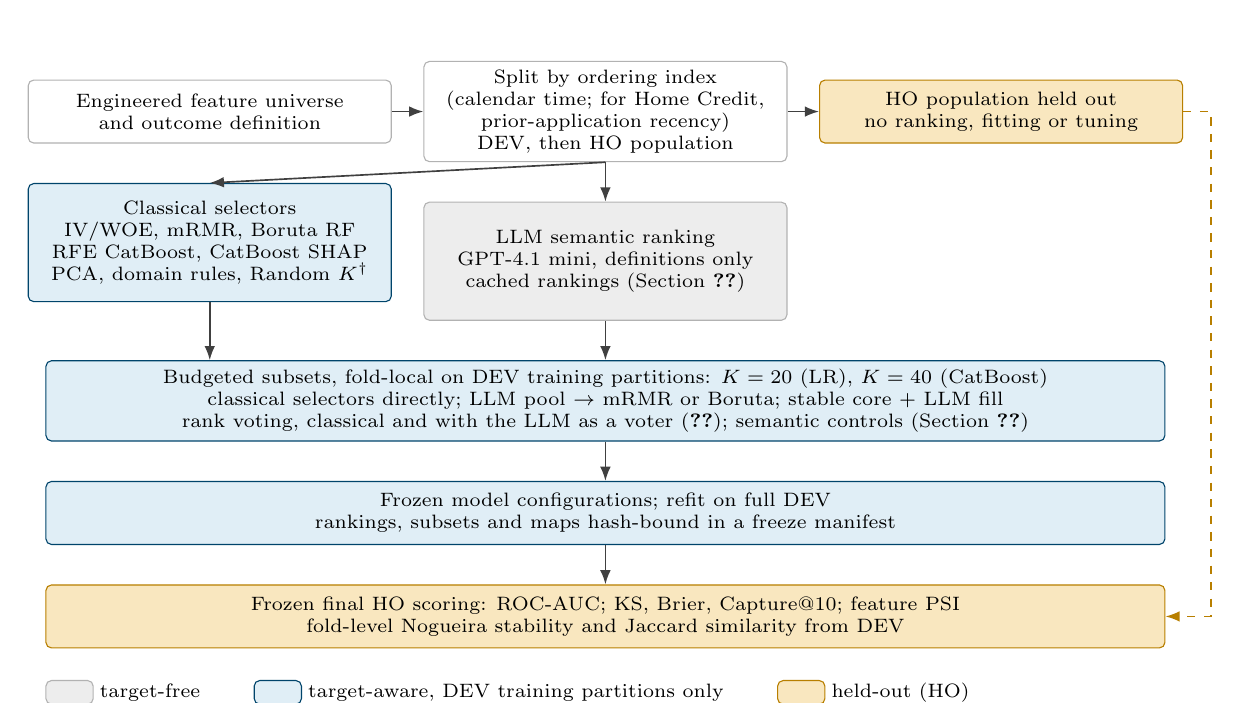
\begin{tikzpicture}[
    font=\scriptsize,
    box/.style={draw=gray!60, rounded corners=2pt, align=flush center, inner sep=3pt, minimum height=8mm, fill=white},
    tfree/.style={box, fill=gray!14},
    taware/.style={box, fill=cBlue!12, draw=cBlue!60!black},
    oot/.style={box, fill=cOrange!25, draw=cOrange!80!black},
    arr/.style={-{Latex[length=1.8mm]}, semithick, gray!50!black},
    darr/.style={-{Latex[length=1.8mm]}, semithick, dashed, cOrange!80!black},
    node distance=5mm and 4mm
]
\node[box, text width=44mm] (data) {Engineered feature universe\\and outcome definition};
\node[box, text width=44mm, right=of data] (split) {Split by ordering index\\(calendar time; for Home Credit,\\prior-application recency)\\DEV, then HO population};
\node[oot, text width=44mm, right=of split] (ootheld) {HO population held out\\no ranking, fitting or tuning};

\node[taware, text width=44mm, minimum height=15mm, below=of data] (classical) {Classical selectors\\IV/WOE, mRMR, Boruta RF\\RFE CatBoost, CatBoost SHAP\\PCA, domain rules, Random $\Kfeat^{\dagger}$};
\node[tfree, text width=44mm, minimum height=15mm, below=of split] (llm) {LLM semantic ranking\\GPT-4.1 mini, definitions only\\cached rankings (Section~\ref{subsec:llm_fs})};

\node[taware, text width=140mm, below=of llm] (subset) {Budgeted subsets, fold-local on DEV training partitions: $\Kfeat=20$ (LR), $\Kfeat=40$ (CatBoost)\\classical selectors directly; LLM pool $\rightarrow$ mRMR or Boruta; stable core + LLM fill\\rank voting, classical and with the LLM as a voter (\ref{app:voting}); semantic controls (Section~\ref{subsec:classical_fs})};
\node[taware, text width=140mm, below=of subset] (model) {Frozen model configurations; refit on full DEV\\rankings, subsets and maps hash-bound in a freeze manifest};
\node[oot, text width=140mm, below=of model] (eval) {Frozen final HO scoring: ROC-AUC; KS, Brier, Capture@10; feature PSI\\fold-level Nogueira stability and Jaccard similarity from DEV};

\draw[arr] (data) -- (split);
\draw[arr] (split) -- (ootheld);
\draw[arr] (split) -- (llm);
\draw[arr] (split.south) -- (classical.north);
\draw[arr] (classical) -- (classical.south |- subset.north);
\draw[arr] (llm) -- (subset);
\draw[arr] (subset) -- (model);
\draw[arr] (model) -- (eval);
\draw[darr] (ootheld.east) -- ++(3.5mm,0) |- (eval.east);

\node[tfree, minimum height=3mm, minimum width=6mm, inner sep=0pt, anchor=north west] (l1) at ([yshift=-4mm]eval.south west) {};
\node[anchor=west, inner sep=2pt] (t1) at (l1.east) {target-free};
\node[taware, minimum height=3mm, minimum width=6mm, inner sep=0pt, anchor=west] (l2) at ([xshift=6mm]t1.east) {};
\node[anchor=west, inner sep=2pt] (t2) at (l2.east) {target-aware, DEV training partitions only};
\node[oot, minimum height=3mm, minimum width=6mm, inner sep=0pt, anchor=west] (l3) at ([xshift=6mm]t2.east) {};
\node[anchor=west, inner sep=2pt] at (l3.east) {held-out (HO)};
\end{tikzpicture}
\caption{Research pipeline. Grey boxes are target-free stages that consume metadata only; blue boxes are target-aware stages confined to DEV training partitions and refitted once on full DEV, except that PCA, domain rules and Random $\Kfeat$ ($\dagger$), grouped with the classical selectors, are themselves target-free; orange boxes concern the held-out population (HO), which the frozen final pipelines score once. Diagram code generated with AI assistance (see the declaration on generative AI).}
\label{fig:pipeline}
\end{figure*}

\subsection{Data Preprocessing}
\label{subsec:preprocessing}

Numeric variables have infinite values set to missing, are imputed with the training-partition mean and are standardised with training-partition statistics. Categorical variables receive an explicit missing token and are one-hot encoded. Levels unseen in the training partition are ignored, and levels rarer than 10 observations (Home Credit, Stability 2024) or 50 (LendingClub) are dropped. Screening and selection operate on \emph{original} features, one column per candidate, so a categorical variable is selected or rejected as a whole, and one-hot expansion follows selection, so the budget $\Kfeat$ counts original variables. Two selectors depart from this order. Principal-component selection retains components, and the statistical stage of LLM then mRMR on LendingClub~v2 operates on the expanded matrix, so its budget counts one-hot columns (Table~\ref{tab:dimension} gives the width of every headline subset). CatBoost receives the same one-hot expansion rather than its native categorical handling, so that one preprocessing map serves both backbones; Section~\ref{subsec:robustness} reports the CatBoost cases re-run with native handling. Maps are fitted on the training partition of each fold and, for the final model, on full DEV.

\subsection{Classical Feature-Selection Methods}
\label{subsec:classical_fs}

Unless stated otherwise, each selector of Table~\ref{tab:methods} ranks the candidates by its own criterion and keeps the top $\Kfeat$ original features. \emph{IV/WOE} ranks by Eq.~\eqref{eq:iv} with ten quantile bins on the training partition \cite{siddiqi2006}, and the same statistic defines the pre-screen of \emph{IV then Boruta}. The \emph{mRMR} selector applies Eq.~\eqref{eq:mrmr} with mutual information estimated on the training partition \cite{peng2005,kraskov2004,ross2014} over the whole candidate set. Throughout, \emph{mRMR} used alone denotes this mutual-information implementation. The random-forest/correlation rule used inside the stable-core construction, as the second stage of LLM then mRMR on Home Credit and LendingClub (Section~\ref{subsec:hybrid_fs}) and in the classical voting family (\ref{app:voting}) is called the \emph{RF/correlation filter}; early versions of the study named it legacy mRMR. \emph{Boruta RF} confirms features whose random-forest importance (500 trees of depth 6) exceeds the best shuffled shadow importance at $\alpha=0.05$ with two-step correction, and keeps the top $\Kfeat$ confirmed features \cite{kursa2010,breiman2001}. When fewer than $\Kfeat$ are confirmed, the subset holds the confirmed features alone and is flagged as below budget; tentative or rejected features are never added. \emph{RFE CatBoost} removes 20\% of the surviving features per step by the importance of an internal CatBoost ranker (500 iterations, depth 6, learning rate 0.05) until $\Kfeat$ remain \cite{guyon2002}. \emph{CatBoost SHAP} keeps the $\Kfeat$ features with the largest aggregate absolute SHAP contribution over a 10,000-row training sample \cite{lundberg2017}. \emph{PCA} retains the leading components as a transformation baseline \cite{jolliffe2016}. \emph{Domain rules} is a deterministic credit-domain scorer that reads no data and calls no model. Its 42 named-variable rules, family and string-pattern rules for bureau, instalment, credit-card and previous-application aggregates, 15 property-attribute rules and nine semantic-group fallbacks assign each feature a priority, adjusted for aggregation suffixes and leakage status, with deterministic tie ordering. The five Home Credit features its leakage rules flag, aggregates of the count of future instalments in the point-of-sale record, all fail the missingness screen, so no selector could have chosen them. The public code repository fixes the remaining details.

Two \emph{diversity controls} test the headline comparison and are not selection strategies; neither enters any family, leader choice or count in this paper. \emph{Family-capped classical} re-runs the HO-rule classical leader of each case with at most $\lceil \Kfeat/F\rceil$ features per source family, where $F$ is the number of source families in the dataset's universe (Table~\ref{tab:methods}), filling the subset in the base selector's own ranking order. \emph{Depth-0 classical} restricts the same leader to the depth-0 candidates of Stability 2024, \texttt{static\_0} and \texttt{static\_cb\_0}. Both are fitted and scored exactly as the selectors are. Where the cap exhausts the base selector's confirmed features before the budget is reached, the subset stays below budget and is flagged, as for Boruta.

Four \emph{semantic controls}, added when the paper was revised, test the semantic ranking in the same way and are likewise not selection strategies: they enter no family, change no leader, and contribute to no headline table and to no input of the case-level test of Section~\ref{subsec:inference}. Each uses the folds, budgets, candidate sets, backbone configurations and seeds of the strategies, makes no new call to the language model, and was fixed in a protocol file, with the rule for reading its result, after the headline results were known and before its own single held-out scoring (\ref{app:protocol}). \emph{Text-embedding ranking} ranks the candidate records of each dataset once, by the cosine similarity between a dedicated text-embedding model's encoding of each record and of one fixed query sentence (\path{BAAI/bge-large-en-v1.5} at a pinned revision, normalised embeddings \cite{xiao2023bge}; the query is reproduced in \ref{app:text_query}); the records are the five label-free fields the language model receives (name, description, source family, lineage formula, semantic group), and the ranking reads no data rows. Its top $\Kfeat$ names form the subset; \emph{text-embedding then filter} takes its top 60 (logistic regression) or 100 (CatBoost) names as the pool and applies the second stage of the frozen LLM-then-mRMR run of the same case. \emph{Contrastive ranking then filter} applies that second stage to the pool of the contrastive-representation selector of the earlier protocol versions (\ref{app:protocol}): MiniLM sentence embeddings of the same records \cite{wang2020minilm,reimers2019}, aligned by a CLIP-style contrastive objective \cite{radford2021} with label-free distribution descriptors of each feature computed on DEV training rows, and ranked by similarity to an anchor set of temporally stable features; it reads rows, without outcomes. \emph{LLM + contrastive fusion} averages the normalised ranks (Eq.~\eqref{eq:normrank}) of the cached semantic ranking of the partition and of the contrastive ranking refitted on the partition's training rows, with equal weight and ties broken by the semantic rank, and keeps the top $\Kfeat$ of the fused ranking; it tests whether a label-free row-reading stage recovers the fold-to-fold reproducibility that the per-fold semantic lists lack (Section~\ref{subsec:stability_results}). The first is compared with pure LLM, the second and third with LLM then mRMR and the fourth with pure LLM, on identical held-out observations with the paired bootstrap of Section~\ref{subsec:inference}; a difference of at least $0.010$ with an interval excluding zero counts as material, and a change of at least $0.05$ in mean fold Jaccard as a change in reproducibility. The rank-voting family of \ref{app:voting} was extended at the same stage by an arm that adds the cached semantic ranking as a fourth equal-weight voter, on all three datasets, read against the same bar.

\begin{table*}[htbp]
\centering
\footnotesize
\begin{threeparttable}
\caption{Feature-selection strategies. ``Labels'' states whether the stage that produces the final subset uses DEV outcomes; ``Datasets'' states where the strategy is evaluated on held-out data. The full-feature model is a reference, not a selector. The two diversity controls and the four semantic controls at the foot test the headline comparison and enter no family, strategy count or leader choice (Section~\ref{subsec:classical_fs}).}
\label{tab:methods}
\begin{tabular}{@{}llL{46mm}cl@{}}
\toprule
Method & Family & Selection role & Labels & Datasets \\
\midrule
Full features & Reference & No selection; context only & -- & All three \\
Domain rules & Classical & Eligibility and policy filters written for the Home Credit variable book & no & All three\tnote{a} \\
Random $\Kfeat$ & Classical & Baseline: uniformly random subset of size $\Kfeat$, the floor for every selector & no & All three \\
PCA & Classical & Leading components of the standardised candidates (components, not original features) & no & All three \\
IV/WOE & Classical & Ranking by information value, Eq.~\eqref{eq:iv} & yes & All three \\
mRMR & Classical & Mutual-information relevance against mutual-information redundancy, Eq.~\eqref{eq:mrmr} & yes & All three \\
Boruta RF & Classical & All-relevant random-forest wrapper with shadow-feature comparison & yes & All three \\
IV then Boruta & Classical & Hybrid: IV eligibility screen followed by Boruta confirmation & yes & All three \\
RFE CatBoost & Classical & Model wrapper: recursive elimination driven by CatBoost importance & yes & All three \\
CatBoost SHAP & Classical & Embedded: ranking by aggregated absolute SHAP contribution & yes & All three \\
Pure LLM & LLM-assisted & Top-$\Kfeat$ names of the cached semantic ranking of the fold & no & All three \\
LLM then mRMR & LLM-assisted & Hybrid: semantic pool of 60 (LR) or 100 (CatBoost), then the RF/correlation filter (Home Credit, LendingClub) or mutual-information mRMR (Stability 2024) & yes & All three \\
LLM then Boruta & LLM-assisted & Hybrid: semantic pool, then Boruta confirmation & yes & All three \\
Stable core + LLM fill & LLM-assisted & Hybrid: bootstrap-stable RF/correlation core completed from the LLM ranking & yes & All three \\
\addlinespace
\multicolumn{5}{@{}l}{\emph{Diversity controls (Section~\ref{subsec:robustness}; not strategies of the comparison)}} \\
Family-capped classical & Control & HO-rule classical leader re-run with at most $\lceil \Kfeat/F\rceil$ features per source family & yes & All three \\
Depth-0 classical & Control & HO-rule classical leader restricted to the depth-0 candidates & yes & Stability 2024 \\
\addlinespace
\multicolumn{5}{@{}l}{\emph{Semantic controls (Section~\ref{subsec:classical_fs}; added at revision; not strategies of the comparison)}} \\
Text-embedding ranking & Control & Top-$\Kfeat$ names by cosine similarity of a text-embedding model (BGE-large) to one fixed query; one ranking per dataset & no & All three \\
Text-embedding then filter & Control & Hybrid: text-embedding pool of 60 (LR) or 100 (CatBoost), then the second stage of LLM then mRMR & yes & All three \\
Contrastive ranking then filter & Control & Hybrid: pool of the contrastive-representation ranking of the earlier protocol versions, then the same second stage & yes\tnote{b} & All three \\
LLM + contrastive fusion & Control & Equal-weight rank fusion of the cached semantic ranking and the contrastive ranking refitted per fold; top $\Kfeat$ & no\tnote{b} & All three \\
\bottomrule
\end{tabular}
\begin{tablenotes}\footnotesize
\item[a] The domain-rules scorer was written around the Home Credit variable book (Section~\ref{subsec:classical_fs}); on LendingClub v2 and Stability 2024 it is applied unchanged and is a portfolio-specific baseline rather than a generic domain baseline (Section~\ref{subsec:cross_dataset}).
\item[b] The contrastive ranking reads DEV training rows (label-free distribution descriptors) but no outcomes, so the two controls built on it are label-free in that stage but not row-free (Section~\ref{subsec:classical_fs}).
\item The rank-voting family of \ref{app:voting}, a supplementary comparison rather than a strategy of this table, covers Home Credit and LendingClub in its pre-declared classical form; its arm with the LLM as a voter, added at revision, covers all three datasets.
\item $F$ is the number of source families in the dataset's universe: 6, 17 and 12. The family cap is 4 ($\Kfeat=20$) and 7 ($\Kfeat=40$) on Home Credit, 2 and 3 on LendingClub, and 2 and 4 on Stability 2024.
\end{tablenotes}
\end{threeparttable}
\end{table*}

\subsection{Pure LLM Selection}
\label{subsec:llm_fs}

The language model is GPT-4.1 mini \cite{openai2025gpt41}, snapshot \path{gpt-4.1-mini-2025-04-14}, called through the Chat Completions interface at temperature 0 with a JSON response format. It never receives rows, outcomes, validation statistics or HO information. One prompt template (\ref{app:prompts}) serves all three datasets under a single \emph{definition-only} information contract: every call used the \texttt{definitions\_only} evidence mode. That mode admits feature names, definitions, source lineage, aggregation operations and observation windows but no numerical summary, so missingness, moments, quantiles, cardinalities and every target-conditioned statistic are withheld; the prompt also forbids remembered dataset-specific results. The descriptions supplied with each candidate record were prepared before ranking and have three provenances. On Home Credit every base definition is the entry of the data dictionary distributed with the competition data, so no analyst phrasing enters it. On LendingClub the first author wrote the definitions of the source columns from the platform's column documentation, and every derived feature (ratio, flag, binned version, interaction, missing indicator) is described by a template from the definitions of its source columns. On Stability 2024 the first author wrote the definitions of the approved raw predictors from the provider's documentation. In all three datasets the feature-engineering code appends to the base definition a clause for the aggregation operation and window, so that a sum over eleven months is described as the total over eleven months; no feature-specific phrasing was added or edited afterwards.

The prompt asks for exactly the requested number of distinct names in priority order. It excludes only features whose supplied definition or lineage reveals the outcome, post-decision information or the evaluation split. Responses are validated strictly: every name must appear verbatim among the candidate records, and the array must hold exactly the requested number of distinct names. A failing response is re-requested up to three times, and no fallback ranking is used.

On Home Credit and LendingClub the ranking is requested separately for each of the five fold training partitions and for full DEV, over the same candidate list in every call (Table~\ref{tab:datasets}). Home Credit has six rankings of 100 names, one per partition, whose prefixes give the budgets of 20, 40, 60 and 100; LendingClub has a separate call per partition and budget, 24 cached rankings. On Stability 2024 one ranking of 100 names over the 1,068 eligible features, accepted at the first attempt, served every fold. Each response is validated, cached and hash-bound, and the cached response, not a fresh call, is the reproducible artefact (Section~\ref{subsec:leakage_controls}). The \emph{pure LLM} selector keeps the top $\Kfeat$ names of the ranking of its partition and budget.

The contract governs the evidence the model may use, not which variables are eligible: eligibility is fixed upstream by the universe assembly and the missingness screen, for every selector alike. The released universes contain fields that fair-lending rules in many jurisdictions treat as protected attributes: applicant gender and family status on Home Credit (\texttt{CODE\_GENDER}, \texttt{NAME\_FAMILY\_STATUS}) and the sex field of the person table on Stability 2024. Age fields also appear, with treatment that differs across regimes. The data providers recorded these categories; the study neither collected nor inferred them and uses them only as released. No exclusion was added to the prompt. An exclusion in the prompt alone would have narrowed the LLM-assisted pool but not the classical one, so the families would no longer share a universe, and any prompt change invalidates the cached rankings behind every LLM-assisted result. A lender's exclusion belongs in the eligibility screen, where it binds every selector; this study applied none and does not evaluate fairness (Section~\ref{subsec:governance}).

To test whether the ranking depends on recognising feature names, the six Home Credit calls were repeated in two obfuscated arms with everything except the feature records held fixed. In arm A every name was replaced by an identifier \texttt{F001}--\texttt{F529} from a seeded permutation of the universe (seed 20260914), drawn per partition so that no identifier carries meaning across calls. Every literal occurrence of the name was also removed from the description, and the identifier-to-name table never entered a prompt. In arm B the names were kept and the descriptions blanked. Each arm's six rankings of 100 identifiers were decoded and carried through the frozen downstream pipeline exactly as the named rankings are, and scored on the same 120,053 HO rows (Section~\ref{subsec:obfuscation_results}).

To test whether the results depend on how the descriptions are phrased, every description of the three candidate sets was rebuilt from lineage alone by a fixed template (raw table, raw variable, depth, aggregation operation, window and type rule), with no statement of credit meaning. The other fields of each record were unchanged. The ranking calls were repeated under the settings of the cached rankings, and the new rankings were carried through the frozen pipelines to the same HO observations (Section~\ref{subsec:mechanical_results}).

\subsection{Hybrid Selection Methods}
\label{subsec:hybrid_fs}

Three hybrids combine the cached semantic ranking with target-aware refinement. \emph{LLM then mRMR} takes the top 60 (logistic regression) or 100 (CatBoost) names of the ranking as the pool and applies a redundancy-aware statistical stage on the fold training partition to reach $\Kfeat$: the RF/correlation filter on Home Credit and LendingClub, whose pipelines were frozen with the implementation of the earlier protocol versions, and mutual-information mRMR on Stability 2024 (\ref{app:protocol}). The semantic stage is meant to remove variables implausible or redundant in meaning, and the statistical stage those redundant in the data. \emph{LLM then Boruta} applies Boruta confirmation to the same pool and truncates to the budget. \emph{Stable core + LLM fill} runs the RF/correlation filter on five bootstrap resamples of the fold training partition (80\% with replacement, seeds 42 to 46). Features selected in at least four of the five form the stable core, ordered by selection frequency and mean rank. The LLM ranking then fills the remaining budget in rank order, without padding from unranked features, so that the core carries reproducibility and semantically prioritised variables fill the rest. The fold-to-fold stability of a hybrid subset depends on both the per-fold semantic ranking and the fitted target-aware stage.

\subsection{Development of the Protocol}
\label{subsec:protocol_development}

% author-confirmed: no held-out population was scored before the final pipelines were frozen; the Stability 2024 cutoff (2020-02-26) was never moved.
The protocol above is the final form of an evaluation developed through successive versions on development data, and its results supersede theirs. Across versions the comparator changed from a single mRMR baseline to the classical family leader of each case, the feature descriptions supplied to the language model were revised, mutual-information mRMR replaced the RF/correlation filter as the stand-alone statistical selector, a contrastive-representation selector that fitted neither family was dropped from the strategy set as out of scope (\ref{app:protocol}; it is reported as a control at revision, Section~\ref{subsec:classical_fs}), and fold-level rank tests gave way to paired bootstrap intervals without observation-level significance claims. Each change was made on development-fold evidence; no held-out population was scored before the final pipelines were frozen, and each frozen pipeline then scored its held-out population once. The three leader rules of Section~\ref{subsec:inference} are read from that single run: the DEV rule, the only development-data rule specified, and the mixed rule, both added when the paper was revised, re-pair selectors already scored in it, without refitting or rescoring and without held-out information in the choice of the pair. The case-level signed-rank test of Section~\ref{subsec:inference}, also added when the paper was revised, is computed from the paired differences of that run alone. The semantic controls of Section~\ref{subsec:classical_fs} and the LLM-vote arm of \ref{app:voting}, added at the same revision, are new pipelines, each fixed in a protocol file after the headline results were known and before its own single held-out scoring; they enter no family and move no value of the headline tables (\ref{app:protocol}). The Stability 2024 cutoff, 2020-02-26, was fixed when the dataset was added and was not moved (Section~\ref{subsec:dev_oot}). \ref{app:protocol} and Table~\ref{tab:stages} give the full account.

% ============================================================
% 5. EXPERIMENTAL SETUP
% ============================================================

\section{Experimental Setup}
\label{sec:experimental_setup}

\subsection{Datasets}
\label{subsec:datasets}

Three public credit datasets released through Kaggle are used (Table~\ref{tab:datasets}); Figure~\ref{fig:scale} shows the scale of the selection problem in each. \emph{Home Credit} is the Home Credit Default Risk data \cite{homecredit2018}: the unit is a loan application, the event is the provider's binary target (payment difficulties), and the universe holds 529 original features derived from the application record and the auxiliary tables. Its ordering index, \texttt{DAYS\_DECISION}, is the number of days between the applicant's most recent previous application and the current one. The split is therefore a recency-based covariate-shift holdout rather than a calendar-time split: DEV holds applicants whose most recent previous application is 241 to 600 days old and HO those with a more recent one. Features that are functions of this index, the previous-application decision days and their aggregates, are outside every selector's candidate set, so no selector could learn on a range of the index that HO does not contain. Applications without a previous application within the 600-day window are excluded. The two windows cover 219,145 of the 307,511 applications in the public release, and the remaining 28.7 per cent are not used, which limits the population to which the Home Credit results apply.

\emph{LendingClub v2} is the LendingClub loan book \cite{lendingclub_kaggle}, restricted to 36- and 60-month loans resolved by the 2019-05-01 snapshot; charged-off or defaulted loans are events and fully paid loans non-events. The 675 features were generated deterministically from roughly 93 distinct columns of the loan book, and each is an attribute of a single loan and its applicant at origination. They comprise 116 raw columns, 180 binary flags, 158 ratios, 88 missing indicators, 78 further engineered variables, 27 binned versions, 19 interactions and 9 categoricals. No feature aggregates across loans or over calendar periods; the only elapsed-time quantity, the months between \texttt{issue\_\allowbreak d} and \texttt{earliest\_\allowbreak cr\_\allowbreak line}, is an attribute of the loan rather than a time index. A prediction-time availability review removed two groups of source columns before any feature was built. The first is every post-origination field, among them \texttt{total\_\allowbreak pymnt}, \texttt{recoveries}, \texttt{last\_\allowbreak pymnt\_\allowbreak amnt}, \texttt{out\_\allowbreak prncp}, the \texttt{last\_\allowbreak fico\_\allowbreak range} fields, \texttt{hardship\_\allowbreak flag} and \texttt{debt\_\allowbreak settlement\_\allowbreak flag}, which would reveal the outcome. The second is the platform's own pricing and grading fields, \texttt{int\_\allowbreak rate}, \texttt{grade}, \texttt{sub\_\allowbreak grade}, \texttt{installment} and \texttt{funded\_\allowbreak amnt}. Excluding them poses the selection problem over applicant and bureau attributes rather than over a re-encoding of a credit decision already taken, at the cost that the AUC levels are not comparable with LendingClub studies that retain the grade or interest rate. Several credit-file attributes were introduced during the sample period, so their missingness, and that of the features derived from them, is higher in DEV than in HO. The highest missingness of any LendingClub feature on the earliest training partition is 82\%, so the screen retains all 675: 566 features fall below 40\%, two lie between 40 and 60\% and 107 between 60 and 82\%. None of them appears anywhere in the cached semantic rankings, so no LLM-assisted subset contains one. The target-aware selectors down-weight them by construction, because a field that is sparse in the DEV training partition carries little information value, mutual information or model importance. The ordering index is the number of days from the issue month to the last finalised issue month, 2018-12-01, so HO is later in calendar time: DEV holds the loans issued from January 2014 to December 2015 and HO those issued in 2016. Thirty-six-month loans account for 445,596 of the 598,649 DEV loans and 232,361 of the 293,105 HO loans. Their event rates are 14.5\% (36-month) and 34.3\% (60-month) in DEV and 19.8\% and 36.4\% in HO, so the DEV--HO difference in event rate arises within both terms, not only from a change in term mix.

\emph{Stability 2024} is the Home Credit Credit Risk Model Stability data \cite{homecredit2024}: the unit is a credit decision dated by \texttt{date\_\allowbreak decision}, and the event is the provider's default target. The 1,959 engineered features were generated deterministically from the 434 approved raw predictors. The training base table defines the population and the case identifier. At depth 0 the two static families, \texttt{static\_\allowbreak 0} and \texttt{static\_\allowbreak cb\_\allowbreak 0}, are joined one-to-one to the base. At depth 1 ten table families have several rows per case: \texttt{applprev\_\allowbreak 1}, \texttt{tax\_\allowbreak registry\_\allowbreak a\_\allowbreak 1}, \texttt{tax\_\allowbreak registry\_\allowbreak b\_\allowbreak 1}, \texttt{tax\_\allowbreak registry\_\allowbreak c\_\allowbreak 1}, \texttt{credit\_\allowbreak bureau\_\allowbreak a\_\allowbreak 1}, \texttt{credit\_\allowbreak bureau\_\allowbreak b\_\allowbreak 1}, \texttt{other\_\allowbreak 1}, \texttt{person\_\allowbreak 1}, \texttt{deposit\_\allowbreak 1} and \texttt{debitcard\_\allowbreak 1}. Each is reduced to one row per case by fixed outcome-independent operations: count, mean, minimum, maximum, standard deviation and the chronologically latest value for numeric and date variables, and mode, most recent category and number of distinct values for categorical ones. Dates are expressed relative to \texttt{date\_\allowbreak decision} where appropriate, future information and depth-2 tables are excluded, and no ratios, interactions or target-informed transformations are introduced. Every generated variable keeps its lineage to raw table, raw variable, depth, operation and type rule, and time windows come from the names of the raw predictors rather than from the engineering. Home Credit and Stability 2024 share institutional lineage, whereas LendingClub is a distinct peer-to-peer platform.

\begin{table*}[htbp]
\centering
\footnotesize
\begin{threeparttable}
\caption{Datasets, held-out partitions and feature universes. The candidate set is the screened universe from which every selector chooses, fixed on the earliest training fold. Windows are days of the most recent previous-application decision relative to the current application (Home Credit), days from the issue month to 2018-12-01 (LendingClub) and calendar dates of \texttt{date\_decision} (Stability 2024).}
\label{tab:datasets}
% author-confirmed: Stability 2024 column = the 2020-02-26 cohort, the only cohort evaluated.
\begin{tabular}{@{}lL{29mm}L{31mm}L{31mm}@{}}
\toprule
 & Home Credit & LendingClub v2 & Stability 2024 \\
\midrule
Observation unit & Loan application & Issued loan & Credit decision \\
Event definition & Payment difficulties (provider target) & Charged off or default; resolved loans only & Default (provider target) \\
DEV window & day $-600$ to $-241$ & day $-1795$ to $-1096$ (issued 2014-01 to 2015-12) & 2019-01-01 to 2020-02-25 \\
DEV $N$ & 99,092 & 598,649 & 1,221,743 \\
DEV event rate & 7.93\% & 19.54\% & 3.24\% \\
HO window & day $-240$ to $-1$ & day $-1065$ to $-730$ (issued 2016-01 to 2016-12) & 2020-02-26 to 2020-10-05 \\
HO $N$ & 120,053 & 293,105 & 304,916 \\
HO event rate & 8.90\% & 23.29\% & 2.74\% \\
Feature universe & 529 original features & 675 engineered features (93 source columns) & 1,959 engineered features \\
Candidate set, all selectors & 373 of 529 ($\le$90\% missing) & 675 of 675 ($\le$90\% missing) & 1,068 of 1,959 ($\le$90\% missing) \\
\bottomrule
\end{tabular}
\end{threeparttable}
\end{table*}

\begin{figure*}[htbp]
\centering
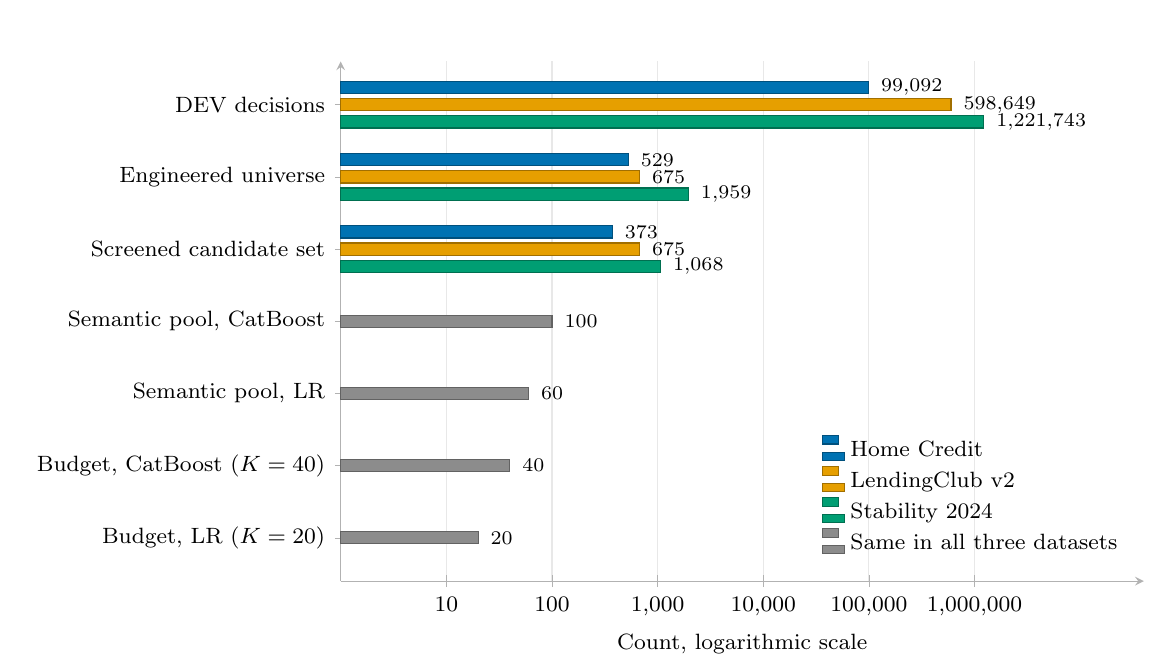
\begin{tikzpicture}
\begin{axis}[
    paper,
  xbar, bar width=4.4pt,
  scale only axis, width=10.2cm, height=6.6cm,
  xmode=log, log basis x=10, xmin=1, xmax=4e7,
  xtick={10,100,1000,10000,100000,1000000},
  xticklabels={10,100,{1,000},{10,000},{100,000},{1,000,000}},
    xmajorgrids, axis lines=left, clip=false,
  xlabel={Count, logarithmic scale},
  symbolic y coords={bLR,bCB,pLR,pCB,cand,univ,dev},
  ytick={bLR,bCB,pLR,pCB,cand,univ,dev},
  yticklabels={{Budget, LR ($\Kfeat=20$)},{Budget, CatBoost ($\Kfeat=40$)},{Semantic pool, LR},{Semantic pool, CatBoost},{Screened candidate set},{Engineered universe},{DEV decisions}},
  enlarge y limits=0.1,
  legend style={at={(0.985,0.03)}, anchor=south east, legend columns=1, cells={anchor=west}},
  reverse legend,
  nodes near coords, point meta=explicit symbolic,
  every node near coord/.append style={font=\scriptsize, anchor=west, xshift=1pt},
]
\addplot[fill=cGrey, draw=cGrey!70!black, bar shift=0pt] coordinates {(20,bLR) [20] (40,bCB) [40] (60,pLR) [60] (100,pCB) [100]};
\addlegendentry{Same in all three datasets}
\addplot[fill=cGreen, draw=cGreen!70!black, bar shift=-6.2pt] coordinates {(1068,cand) [1{,}068] (1959,univ) [1{,}959] (1221743,dev) [1{,}221{,}743]};
\addlegendentry{Stability 2024}
\addplot[fill=cOrange, draw=cOrange!70!black, bar shift=0pt] coordinates {(675,cand) [675] (675,univ) [675] (598649,dev) [598{,}649]};
\addlegendentry{LendingClub v2}
\addplot[fill=cBlue, draw=cBlue!70!black, bar shift=6.2pt] coordinates {(373,cand) [373] (529,univ) [529] (99092,dev) [99{,}092]};
\addlegendentry{Home Credit}
\end{axis}
\end{tikzpicture}
\caption{Scale of the selection problem in each dataset: the development (DEV) decisions on which every supervised selector is refitted, the engineered universe, the screened candidate set offered to every selector, the semantic pool that the hybrids hand to their statistical stage (60 names for logistic regression, 100 for CatBoost) and the budget ($\Kfeat=20$ and $\Kfeat=40$); the pool and the budget are the same in all three datasets. Logarithmic axis. Plot code generated with AI assistance (see the declaration on generative AI).}
\label{fig:scale}
\end{figure*}

\subsection{Held-Out DEV/HO Design}
\label{subsec:dev_oot}

Each dataset is split along its ordering index into a development population (DEV) and a held-out population (HO). On LendingClub and Stability 2024 the index is calendar time and HO is later than DEV. The design asks whether a selected subset and a fitted model still rank risk on loans issued or decisions taken after development, which random splits would mask \cite{bergmeir2012,gama2014}. The split orders decisions, not outcomes. Because the provider-defined outcome horizons are not fully specified, this chronological holdout does not by itself show that every development label would have been observable at the held-out decision dates, as a fully simulated deployment would require. On Home Credit the index is prior-application recency, so HO holds applicants with a more recent previous application, not later applications. Its event rate is higher, 8.90\% against 7.93\% in DEV (Table~\ref{tab:datasets}), so the frozen pipelines must rank risk in a subgroup that is both differently distributed and riskier, a harder target than a shift in covariates alone. The split point was fixed on the index rather than on a target share of the population. The Home Credit HO population (120,053 applications from a 240-day recency window) is therefore larger than DEV (99,092 from a 360-day window), recent previous applications being denser in the release. An equal split was rejected because moving the cut to balance the two sides would have set it with knowledge of the population it defines.

Within DEV, five expanding-window folds are formed along the same index. Each training partition holds the lowest-index observations and the validation partition a later block, with one index unit assigned to neither: a day on Home Credit and LendingClub, and a decision date on Stability 2024, so same-date decisions stay together. This unit is not a calendar embargo. LendingClub is indexed by issue month, so there it separates the partitions by position in the ordering rather than by elapsed time; the ordered split itself keeps later loans out of training. On Home Credit the folds follow the recency index for consistency with the other datasets, not to simulate the passage of time. Every component is fitted on the training partition, applied to the validation partition without refitting, and refitted once on full DEV.

% author-confirmed: the Stability 2024 cutoff is 2020-02-26 and was never moved; every Stability 2024 result in this paper belongs to this cohort.
On Stability 2024 the HO cutoff is 2020-02-26, fixed when the dataset was added to the study and not moved thereafter (Section~\ref{subsec:protocol_development}). DEV comprises the 1,221,743 decisions dated 2019-01-01 to 2020-02-25 (event rate 3.24\%) and HO the 304,916 decisions dated 2020-02-26 to 2020-10-05 (8,349 events, 2.74\%), 20.0\% of the 1,526,659 decisions. The HO population is therefore lower-risk than DEV, the reverse of Home Credit, and the cut was not moved to balance the two sides for the reason given there: doing so would have set it with knowledge of the population it defines. On LendingClub the HO window runs from day $-1065$ to day $-730$ (loans issued from 2016-01 through 2016-12), and loans unresolved at the 2019-05-01 snapshot are excluded. This restriction can preferentially retain early defaults and early repayments while other loans of the same cohort remain unresolved, and follow-up differs across issue cohorts and between the two terms. Population composition and the DEV--HO event-rate difference should be read with this selection in mind; the LendingClub findings describe the resolved-loan population.

\subsection{Predictive Models}
\label{subsec:models}

Two backbones are used in every case, a linear scorecard-style model and a non-linear boosted model \cite{lessmann2015,gunnarsson2021}, with configurations fixed and identical across selectors. Logistic regression (LR) uses the \texttt{liblinear} solver of scikit-learn \cite{pedregosa2011} with an L2 penalty, $C=1$, at most 1,000 iterations, balanced class weights and random seed 42. CatBoost \cite{prokhorenkova2018} uses depth 10, learning rate 0.01, L2 leaf regularisation 95, at least 290 observations per leaf, a feature-sampling rate (\texttt{rsm}) of 0.90 and random strength 0.125. It grows depthwise, uses Bernoulli bootstrap with subsample 0.55, the Logloss objective with AUC evaluation, balanced class weights, seed 42 and four threads, and runs a fixed 1,500 iterations without early stopping, so that no validation information enters the fitted model. Class weights are balanced because event rates range from about 3\% to 23\%. The same configurations serve every feature count, from the 20- and 40-feature subsets to the full-feature reference models on 373, 675 and 1,959 features, the Stability 2024 references being fitted on the unscreened universe. The CatBoost configuration was carried over unchanged from the authors' prior credit-scoring work at the Central Bank of the Republic of Uzbekistan on a separate, non-public portfolio, where it had been tuned on a validation set. No hyperparameter of either backbone was tuned on any partition of the three datasets. The full-feature reference was not tuned separately either, so the ``Full'' column of Table~\ref{tab:primary_results} is a context model under the compact configuration, not a tuned upper bound.

\subsection{Feature Budgets}
\label{subsec:feature_budgets}

The budgets, $\Kfeat=20$ original features for logistic regression and $\Kfeat=40$ for CatBoost, were set in DEV-only experiments and frozen before HO evaluation. Larger linear subsets raised development AUC only marginally, by $+0.004$ on average at $\Kfeat=30$ and $+0.005$ at $\Kfeat=40$ for one and a half to two times the feature count, so $\Kfeat=20$ became the compact operating point. CatBoost gained up to $\Kfeat=40$ and nothing further on average, and it was less sensitive to redundant predictors. The budget sets the level of every selector in a case without changing the order of the two families, except at $\Kfeat=10$ on Stability 2024 with logistic regression (\ref{app:budgets}). Budgets are model-specific, so selectors are compared at equal subset size within a backbone, while comparisons between backbones differ in both model class and budget. Equal subset size is not equal input width once categoricals are expanded (Table~\ref{tab:dimension}).

\subsection{Evaluation Metrics}
\label{subsec:metrics}

Let $y_i\in\{0,1\}$ be the event label of HO observation $i$, $p_i$ its predicted event probability, $N_+$ and $N_-$ the numbers of events and non-events, and $N=N_++N_-$.

\paragraph{ROC-AUC}
The area under the receiver operating characteristic curve is the probability that a randomly chosen event scores higher than a randomly chosen non-event, with half credit for ties \cite{hanley1982},
\begin{equation}
    \AUC=\frac{1}{N_+N_-}\sum_{i:\,y_i=1}\sum_{j:\,y_j=0}\big[\mathbf{1}(p_i>p_j)+\tfrac12\mathbf{1}(p_i=p_j)\big].
    \label{eq:roc_auc}
\end{equation}
Higher is better. ROC-AUC is threshold-free and is the sole headline metric; the Gini coefficient $2\,\AUC-1$ adds no information.

\paragraph{KS}
The Kolmogorov--Smirnov statistic is the maximum vertical separation between the cumulative score distributions of events and non-events,
\begin{equation}
    \KS=\max_{t}\,\big[\TPR(t)-\FPR(t)\big],
    \label{eq:ks}
\end{equation}
which equals the maximum Youden index over thresholds \cite{youden1950}; higher is better. KS is reported as the maximum HO separation. Each freeze manifest also records a KS-optimal threshold for deployment, but no threshold-dependent metric is reported.

\paragraph{Brier score}
The Brier score is the mean squared error of the predicted probabilities \cite{brier1950},
\begin{equation}
    \mathrm{Brier}=\frac{1}{N}\sum_{i=1}^{N}(y_i-p_i)^2 ,
    \label{eq:brier}
\end{equation}
lower is better. It combines calibration and resolution rather than measuring ranking; a constant prediction equal to the event rate $\pi$ attains $\pi(1-\pi)$, and log loss, $-N^{-1}\sum_i[y_i\ln p_i+(1-y_i)\ln(1-p_i)]$, is a supporting diagnostic. Both backbones use balanced class weights and no recalibration (Section~\ref{subsec:models}), so their outputs are not population event probabilities: Brier values compare selectors within a dataset and do not indicate deployment-ready calibration.

\paragraph{Capture@10 and Lift@10}
Let $T$ be the set of observations in the highest-scored decile, a fraction $q=|T|/N\approx0.10$ of the population. Capture@10 is the share of all events found in that decile and Lift@10 the ratio of the decile event rate to the portfolio event rate,
\begin{equation}
\begin{aligned}
    \mathrm{Capture@10}&=\frac{\sum_{i\in T}y_i}{\sum_{i}y_i},\\
    \mathrm{Lift@10}&=\frac{|T|^{-1}\sum_{i\in T}y_i}{N^{-1}\sum_{i}y_i}=\frac{\mathrm{Capture@10}}{q};
\end{aligned}
    \label{eq:capture10}
\end{equation}
higher is better, and Lift equals ten times Capture only when the decile is exact.

\paragraph{PSI}
The population stability index compares a reference distribution with a later distribution over frozen states $b$,
\begin{equation}
    \PSI=\sum_{b}\big(o_b-r_b\big)\ln\frac{o_b}{r_b},
    \label{eq:psi}
\end{equation}
where $r_b$ and $o_b$ are the reference (DEV) and HO proportions in state $b$ \cite{siddiqi2006,yurdakul2020}; lower indicates less shift. PSI is reported for the selected features only; a score PSI computed in earlier drafts of this paper from the same run, which compared out-of-fold DEV scores of the fold models with HO scores of the full-DEV refit, mixed scoring-model differences with population change and is not reported. For \emph{feature PSI} the states are type-aware: DEV quantile bins plus a missing state for continuous variables, explicit 0/1/missing/unexpected states for binary and one-hot variables, exact DEV levels for discrete variables, and DEV categories plus missing and unseen states for source categoricals. Bins and states are learned on DEV, frozen and applied unchanged to HO, and the mean, median and maximum feature PSI over a subset summarise its drift. A feature PSI of zero means that no difference was detected under the implemented states, binning and numerical precision, not that the distributions are identical. The conventional references of 0.10 and 0.25 are monitoring thresholds, not critical values \cite{yurdakul2020}.

\paragraph{Nogueira stability}
Let $Z_{fj}\in\{0,1\}$ indicate whether feature $j$ of a candidate universe of size $d$ is selected in the $f$-th of $B$ selected subsets, $f=1,\dots,B$. The subsets are the five development folds, $B=5$, except for the ten repeated responses to one fixed prompt of Section~\ref{subsec:stability_results}, $B=10$. With $\hat p_j=B^{-1}\sum_f Z_{fj}$, $s_j^2=\frac{B}{B-1}\hat p_j(1-\hat p_j)$ and $\bar k=\sum_j \hat p_j$, the Nogueira estimator is \cite{nogueira2018}
\begin{equation}
    \hat\Phi=1-\frac{d^{-1}\sum_{j=1}^{d}s_j^2}{(\bar k/d)\,(1-\bar k/d)} .
    \label{eq:nogueira}
\end{equation}
It equals 1 when the same subset is selected in every fold, is chance-corrected so that random selection gives values near 0, and can be negative. The universe $d$ is the pool from which the fold-local selector chose, the screened candidate set (373, 675 or 1,068 features), for the classical selectors, the LLM hybrids and the pure LLM lists alike.

\paragraph{Jaccard similarity}
For fold subsets $S_a$ and $S_b$ the Jaccard similarity is $J(S_a,S_b)=|S_a\cap S_b|/|S_a\cup S_b|$ \cite{jaccard1901}. Mean pairwise Jaccard averages $J$ over the $B(B-1)/2$ unordered pairs, ten for the five folds and forty-five for the ten repeated responses; higher indicates more reproducible selection. For the fold subsets the minimum and maximum over the ten pairs are reported as the fold-pair spread. Unlike Eq.~\eqref{eq:nogueira}, $J$ is not chance-corrected and does not depend on $d$, so the two statistics are reported together.

\subsection{Statistical Inference}
\label{subsec:inference}

Six paired comparisons, one per dataset and backbone, are reported under three rules for choosing the compared methods. Under the \emph{HO rule} (Table~\ref{tab:primary_results}), the LLM-assisted family leader, the LLM-assisted selector with the highest observed HO AUC, is compared with the classical family leader chosen in the same way. The method matrices, budgets and procedure were fixed before HO scoring, but the two leaders were identified from the HO results themselves, so this comparison is descriptive; no observation-level test is reported, no significance is claimed, and the case-level test below inherits that selection. Under the \emph{DEV rule} (Table~\ref{tab:confirmatory}), each family's leader is the selector with the highest mean validation AUC over the five DEV folds, and the two are compared once on HO; the holdout plays no part in the choice. The \emph{mixed rule} pairs the DEV-rule LLM-assisted leader with the HO-rule classical leader, the least favourable pairing for the LLM-assisted family (Section~\ref{subsec:primary_results}).

In every comparison the two pipelines are scored on identical HO observations, paired by observation identifier (\texttt{SK\_\allowbreak ID\_\allowbreak CURR} on Home Credit, a stable identifier derived from the processed source row on LendingClub, the decision identifier on Stability 2024). The paired HO ROC-AUC difference, LLM-assisted minus classical, carries a 95\% interval from 2,000 target-stratified paired bootstrap resamples that draw the same observation indices for both pipelines \cite{efron1993}, with seed 20260721. The interval describes the sampling variability of the difference on the HO population. Under the HO rule it is not adjusted for the selection of the compared pipelines, and under no rule does it cover the sampling of the language model, because each resample holds the cached ranking, and hence the LLM-assisted subset, fixed. That component is measured separately and reported beside the intervals, not inside them, so that the two sources of variation stay distinguishable (Section~\ref{subsec:stability_results}). Comparisons with the full-feature reference and among secondary metrics are point estimates. Large HO samples make small differences detectable, so effect sizes are always reported with the intervals \cite{demsar2006}. A paired AUC difference of at least $0.010$, two Gini points, is treated as material; this \emph{materiality bar} is used throughout, and smaller differences are reported but not counted as a result in either direction. The bar applies to a difference computed from one cached semantic ranking. Where several responses exist it is also applied to the spread of the LLM-assisted AUC across them, a spread below $0.010$ being treated as immaterial response sampling.

No observation-level $p$-value is attached to the headline comparisons. A paired DeLong test, like the paired bootstrap, treats the two fitted pipelines as fixed and asks how the AUC difference would vary if the HO observations were resampled. With 120,053 to 304,916 paired observations that question is answered to the fourth decimal, so every headline difference would be significant at any conventional level and the test would report the size of the holdout rather than anything about the methods. The variation that bears on the claims lies elsewhere. There are three portfolios from at most two independent lenders (Section~\ref{subsec:limitations}), one prompt, one language-model response per case in the headline tables (Section~\ref{subsec:stability_results}) and one seed. No observation-level test resamples these, and the DEV and mixed rules re-pair selectors already scored in the single held-out run (Section~\ref{subsec:protocol_development}). The headline comparison is therefore tested at the level at which it is claimed, the case. Under each rule the six paired differences, one per dataset--backbone case, enter an exact Wilcoxon signed-rank test of a zero median difference \cite{demsar2006}, evaluated on the full null distribution of the $2^6=64$ sign assignments. Two-sided $p$-values are primary, because the direction of the test was not declared before the held-out run, and one-sided values in favour of the LLM-assisted family are reported beside them. The DEV-rule test is the cleanest of the three, because its pair is fixed without held-out information; the HO-rule test inherits the selection of its pair, and the mixed rule inherits it on the classical side. The test was added when the paper was revised and uses only the differences of Tables~\ref{tab:primary_results} and \ref{tab:confirmatory}, with no refitting or rescoring. Its resolution is limited by construction. With six cases the smallest attainable two-sided $p$-value is $2/64=0.031$, reached only when all six differences share a sign; the cases are not independent, since each dataset contributes two backbones and Home Credit and Stability 2024 share institutional lineage; and with the two backbones averaged, three dataset-level differences admit only $2^3=8$ sign assignments, so no exact signed-rank or sign test on them can fall below a one-sided $p$-value of $1/8=0.125$. All three rules are therefore read against the bar and the interval, and the case-level test states how far six cases can carry the comparison. The two-sided paired DeLong test \cite{delong1988} with Holm's step-down adjustment \cite{holm1979} is used only for the rank-voting comparisons of \ref{app:voting}, the pre-declared classical family and its arm with the LLM as a voter, each fixed in a protocol file before its held-out scoring; there every case is decided by the materiality bar, which the Holm condition never binds. The semantic controls of Section~\ref{subsec:classical_fs} are reported with paired bootstrap intervals only.

\subsection{Leakage and Reproducibility Controls}
\label{subsec:leakage_controls}

Leakage controls operate at three levels. HO rows are excluded from every screening, selection, ranking and tuning step, and every target-aware component is fitted fold-locally inside DEV and refitted once on full DEV. Cached rankings, subsets, preprocessing maps, model settings and fitted models are frozen and hash-bound before each final HO scoring run, after which HO rows enter only the computation of the reported metrics. Every frozen final pipeline scored its held-out population once, and the pipelines added at revision (Section~\ref{subsec:classical_fs}; \ref{app:voting}) were each scored once in the same way, with no headline value recomputed (Section~\ref{subsec:protocol_development}). Randomness is controlled by fixed seeds: 42 for both classifiers and the selectors, 42 to 46 for the stable-core resamples and 20260721 for the inference bootstrap. Temperature 0 with a fixed snapshot does not make the language model deterministic; it is the caching of the rankings that makes the reported LLM results reproducible, and Section~\ref{subsec:stability_results} measures the residual variation. Experiments ran in Python 3.13.5 with scikit-learn 1.8.0, CatBoost 1.2.10 and Boruta 0.4.3 on a laptop with an Intel Core i7-13620H processor, one experiment and one fold at a time (Section~\ref{subsec:cost_runtime}). The datasets are public, and code, configuration files and experiment artefacts are in the repository listed in the Data availability statement.

% ============================================================
% 6. RESULTS
% ============================================================

\section{Results}
\label{sec:results}

\subsection{Headline comparison}
\label{subsec:primary_results}

Under the HO rule the LLM-assisted leader has the higher held-out AUC in five of the six cases (Table~\ref{tab:primary_results}, Figure~\ref{fig:primary}). It is pure LLM in four cases, LLM then mRMR in one and stable core plus LLM fill on Home Credit LR, the one case the classical leader wins, by $0.021$. With the cached rankings the five positive margins run from $+0.012$ to $+0.051$ and all clear the materiality bar in point estimate; only the smallest, on Home Credit CatBoost, has an interval reaching below it ($[+0.009, +0.015]$). The classical leader changes identity across cases (mRMR, RFE CatBoost, IV then Boruta or CatBoost SHAP), so a single classical baseline would have represented classical selection differently in each case.

Under the DEV rule (Table~\ref{tab:confirmatory}) the compared pair changes in five of the six cases, but the outcome does not: the LLM-assisted leader is higher in the same five cases, by $+0.014$ to $+0.052$, five margins being wider than under the HO rule. The classical leader keeps Home Credit LR by $0.010$, at the bar (interval $[-0.013, -0.008]$). The rule changes the classical leader in five cases and the LLM-assisted leader on Home Credit LR, to LLM then mRMR; only Stability 2024 LR keeps its pair, pure LLM against RFE CatBoost, and its difference. On Stability 2024 CatBoost the DEV rule prefers the classical selector (0.8635 against 0.8598 on DEV), yet pure LLM is higher on HO by $+0.029$.

The two rules share five of their six LLM-assisted leaders, so the mixed rule can be read from the same tables. In five cases it gives the pair of Table~\ref{tab:primary_results}, with that table's difference and interval. On Home Credit LR it pairs LLM then mRMR with mRMR, a difference of $-0.027$ reported as a point estimate, its interval not computed. The five-of-six pattern therefore holds under all three rules, and under the mixed rule the LLM-assisted margins are those of the HO rule.

The rules are not independent checks, as the DEV and HO values of Table~\ref{tab:confirmatory} show. Choosing a leader on development data can only lower or preserve its HO AUC relative to the HO-best selector of its family, and it costs the two families unequally. The DEV-chosen classical leader is the HO-best classical selector only on Stability 2024 LR and falls $0.001$ to $0.017$ short of it in the other five cases. The DEV-chosen LLM-assisted leader is the HO-best one in five cases and $0.006$ below it on Home Credit LR. The DEV rule widens the margins because it costs the classical family more, not because the LLM-assisted leaders rise (Section~\ref{subsec:dev_to_ho}).

Across the six cases the comparison is consistent in direction, but six cases are too few for a conventional test to confirm it at the 5\% level (Section~\ref{subsec:inference}). Under the DEV rule, whose pair is chosen without held-out information, the one negative difference, Home Credit LR ($-0.010$), is the smallest of the six in absolute size, so the signed-rank statistic is $W^{+}=20$ of a possible 21, with exact two-sided $p=0.063$ and one-sided $p=0.031$, the second-smallest values attainable with six cases. Under the HO rule, whose test inherits the selection of the pair, the negative difference ($-0.021$) is the fourth largest of the six, so $W^{+}=17$, with two-sided $p=0.219$ (one-sided 0.109); the mixed rule, whose negative difference ($-0.027$) also ranks fourth, gives the same values. The five-of-six result is read in that sense throughout: a direction consistent in five of six cases with material margins, at the resolution that six cases from three portfolios allow.

\begin{table*}[htbp]
\centering
\scriptsize
\setlength{\tabcolsep}{3pt}
\begin{threeparttable}
\caption{Primary held-out (HO) comparison under the HO rule. In each case the LLM-assisted and the classical family leader, the selectors with the highest observed HO AUC in their families, are compared on identical HO observations; both were chosen on the HO results, so the differences are descriptive and their intervals are not adjusted for that selection (Section~\ref{subsec:inference}). AUC is shown to four decimals; $\Delta$AUC, LLM-assisted minus classical, and its paired 95\% bootstrap interval are computed at full precision, the Stability 2024 differences being shown to four decimals. ``Full'' is the HO AUC of the untuned full-feature reference, context only (Section~\ref{subsec:models}). The PSI columns give the mean DEV-versus-HO PSI of the features selected by each leader's frozen full-DEV refit; lower is less drift.}
\label{tab:primary_results}
\begin{tabular}{@{}L{24mm}L{27mm}L{24mm}rL{38mm}rr@{}}
\toprule
Case & LLM-assisted leader (AUC) & Classical leader (AUC) & Full & $\Delta$AUC [95\% CI] & PSI\newline LLM & PSI\newline classical \\
\midrule
Home Credit, LR & Stable core + LLM fill\newline (0.7489) & mRMR\newline (0.7699) & 0.7715 & $-0.021033$\newline $[-0.022211,\,-0.019780]$ & 0.0053 & 0.0085 \\
\addlinespace
Home Credit, CatBoost & Pure LLM\newline (0.7935) & RFE CatBoost\newline (0.7814) & 0.7860 & $+0.012024$\newline $[+0.009313,\,+0.014841]$ & 0.0045 & 0.0097 \\
\addlinespace
LendingClub v2, LR & Pure LLM\newline (0.7402) & IV then Boruta\newline (0.7098) & 0.7109 & $+0.030431$\newline $[+0.029359,\,+0.031514]$ & 0.0125 & 0.0129 \\
\addlinespace
LendingClub v2, CatBoost & LLM then mRMR\newline (0.7707) & IV then Boruta\newline (0.7201) & 0.7230 & $+0.050517$\newline $[+0.049712,\,+0.051315]$ & 0.0104 & 0.0125 \\
\addlinespace
Stability 2024, LR & Pure LLM\newline (0.8322) & RFE CatBoost\newline (0.8181) & 0.7659 & $+0.0141$\newline $[+0.012823,\,+0.015339]$ & 0.0174 & 0.0092 \\
\addlinespace
Stability 2024, CatBoost & Pure LLM\newline (0.8716) & CatBoost SHAP\newline (0.8509) & 0.8198 & $+0.0207$\newline $[+0.017219,\,+0.023151]$ & 0.0109 & 0.0189 \\
\bottomrule
\end{tabular}
\end{threeparttable}
\end{table*}

\begin{table*}[htbp]
\centering
\scriptsize
\setlength{\tabcolsep}{3pt}
\begin{threeparttable}
\caption{Held-out (HO) comparison under the DEV rule. In each case the LLM-assisted and the classical family leader are the selectors with the highest mean validation AUC over the five DEV folds in their families, compared once on identical HO observations. Each leader shows its DEV mean and, after the semicolon, its HO AUC; $\Delta$AUC, LLM-assisted minus classical, carries its paired 95\% bootstrap interval (the Stability 2024 differences are shown to four decimals). Unlike the HO-rule comparison of Table~\ref{tab:primary_results}, which is descriptive with intervals not adjusted for selection, the holdout plays no part in the choice here; the rule re-pairs selectors already scored in the single held-out run, with no refitting (Section~\ref{subsec:inference}).}
\label{tab:confirmatory}
\begin{tabular}{@{}L{24mm}L{30mm}L{27mm}L{38mm}@{}}
\toprule
Case & LLM-assisted leader (DEV; HO) & Classical leader (DEV; HO) & $\Delta$AUC [95\% CI] \\
\midrule
Home Credit, LR & LLM then mRMR\newline (0.7472; 0.7432) & IV then Boruta\newline (0.7652; 0.7534) & $-0.010179$\newline $[-0.012863,\,-0.007592]$ \\
\addlinespace
Home Credit, CatBoost & Pure LLM\newline (0.7917; 0.7935) & IV then Boruta\newline (0.7770; 0.7688) & $+0.024700$\newline $[+0.021656,\,+0.027770]$ \\
\addlinespace
LendingClub v2, LR & Pure LLM\newline (0.7436; 0.7402) & RFE CatBoost\newline (0.7211; 0.6989) & $+0.041353$\newline $[+0.040619,\,+0.042072]$ \\
\addlinespace
LendingClub v2, CatBoost & LLM then mRMR\newline (0.7811; 0.7707) & RFE CatBoost\newline (0.7347; 0.7190) & $+0.051702$\newline $[+0.050900,\,+0.052499]$ \\
\addlinespace
Stability 2024, LR & Pure LLM\newline (0.8302; 0.8322) & RFE CatBoost\newline (0.8178; 0.8181) & $+0.0141$\newline $[+0.012823,\,+0.015339]$ \\
\addlinespace
Stability 2024, CatBoost & Pure LLM\newline (0.8598; 0.8716) & RFE CatBoost\newline (0.8635; 0.8425) & $+0.0291$\newline $[+0.027974,\,+0.030174]$ \\
\bottomrule
\end{tabular}
\end{threeparttable}
\end{table*}

\begin{table*}[htbp]
\centering
\footnotesize
\begin{threeparttable}
\caption{Held-out (HO) ROC-AUC of every selector of the two families ($\Kfeat=20$ for logistic regression, $\Kfeat=40$ for CatBoost). Bold marks the HO-rule family leader of each column; the last row is the $\Delta$AUC of Table~\ref{tab:primary_results} rounded to three decimals.}
\label{tab:full_matrix}
\setlength{\tabcolsep}{5pt}
\begin{tabular}{@{}lrrrrrr@{}}
\toprule
 & \multicolumn{2}{c}{Home Credit} & \multicolumn{2}{c}{LendingClub v2} & \multicolumn{2}{c}{Stability 2024} \\
\cmidrule(lr){2-3}\cmidrule(lr){4-5}\cmidrule(l){6-7}
Selector & LR & CatBoost & LR & CatBoost & LR & CatBoost \\
\midrule
\multicolumn{7}{@{}l}{\emph{Classical family (nine selectors)}} \\
Domain rules & 0.7230 & 0.7293 & 0.5525 & 0.6128 & 0.7371 & 0.7791 \\
Random $\Kfeat$ & 0.6278 & 0.6854 & 0.6038 & 0.6718 & 0.6818 & 0.7502 \\
PCA & 0.6838 & 0.7091 & 0.6624 & 0.6787 & 0.7019 & 0.7692 \\
IV/WOE & 0.7381 & 0.7686 & 0.6821 & 0.7027 & 0.7781 & 0.8187 \\
mRMR & \textbf{0.7699} & 0.7599 & 0.6859 & 0.7020 & 0.7769 & 0.8308 \\
Boruta RF & 0.7397 & 0.7542 & 0.6557 & 0.6857 & 0.7611 & 0.8095 \\
IV then Boruta & 0.7534 & 0.7688 & \textbf{0.7098} & \textbf{0.7201} & 0.7976 & 0.8387 \\
RFE CatBoost & 0.7465 & \textbf{0.7814} & 0.6989 & 0.7190 & \textbf{0.8181} & 0.8425 \\
CatBoost SHAP & 0.7501 & 0.7795 & 0.6965 & 0.7151 & 0.8092 & \textbf{0.8509} \\
\addlinespace
\multicolumn{7}{@{}l}{\emph{LLM-assisted family (four pipelines)}} \\
Pure LLM & 0.7436 & \textbf{0.7935} & \textbf{0.7402} & 0.7335 & \textbf{0.8322} & \textbf{0.8716} \\
LLM then mRMR & 0.7432 & 0.7758 & 0.7179 & \textbf{0.7707} & 0.8112 & 0.8519 \\
LLM then Boruta & 0.7337 & 0.7657 & 0.6793 & 0.7002 & 0.8098 & 0.8385 \\
Stable core + LLM fill & \textbf{0.7489} & 0.7809 & 0.7048 & 0.7277 & 0.8171 & 0.8489 \\
\midrule
LLM-assisted leader $-$ classical leader & $-0.021$ & $+0.012$ & $+0.030$ & $+0.051$ & $+0.014$ & $+0.021$ \\
\bottomrule
\end{tabular}
\end{threeparttable}
\end{table*}

\begin{figure*}[htbp]
\centering
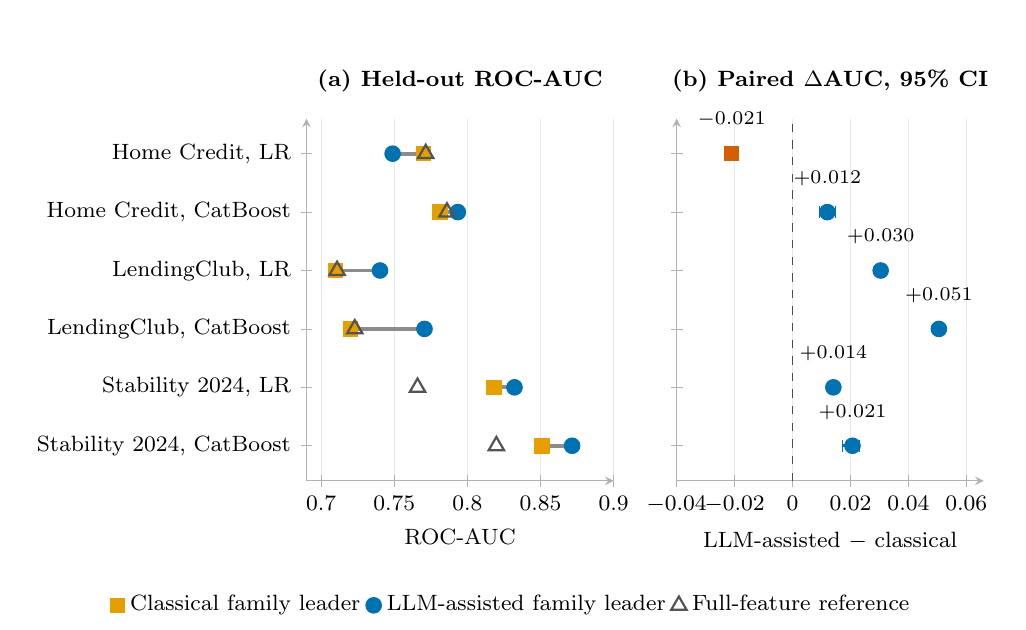
\begin{tikzpicture}
\begin{groupplot}[
    paper,
    group style={group size=2 by 1, horizontal sep=8mm, y descriptions at=edge left},
    scale only axis, width=3.9cm, height=4.6cm,
    ymin=0.4, ymax=6.6, ytick={1,2,3,4,5,6},
    yticklabels={{Stability 2024, CatBoost},{Stability 2024, LR},{LendingClub, CatBoost},{LendingClub, LR},{Home Credit, CatBoost},{Home Credit, LR}},
    xmajorgrids, axis lines=left, clip=false,
    xticklabel style={/pgf/number format/fixed, /pgf/number format/precision=2},
]
\nextgroupplot[title={(a) Held-out ROC-AUC}, xlabel={ROC-AUC}, xmin=0.69, xmax=0.90, xtick={0.70,0.75,0.80,0.85,0.90},
    legend to name=primlegend, legend columns=3]
\addplot[cGrey, line width=1.4pt, forget plot] coordinates {(0.8509,1) (0.8716,1)};
\addplot[cGrey, line width=1.4pt, forget plot] coordinates {(0.8181,2) (0.8322,2)};
\addplot[cGrey, line width=1.4pt, forget plot] coordinates {(0.720147,3) (0.770664,3)};
\addplot[cGrey, line width=1.4pt, forget plot] coordinates {(0.709803,4) (0.740234,4)};
\addplot[cGrey, line width=1.4pt, forget plot] coordinates {(0.781426,5) (0.793450,5)};
\addplot[cGrey, line width=1.4pt, forget plot] coordinates {(0.769890,6) (0.748857,6)};
\addplot[only marks, mark=square*, mark size=2.6pt, cOrange]
    coordinates {(0.8509,1) (0.8181,2) (0.720147,3) (0.709803,4) (0.781426,5) (0.769890,6)};
\addlegendentry{Classical family leader}
\addplot[only marks, mark=*, mark size=2.8pt, cBlue]
    coordinates {(0.8716,1) (0.8322,2) (0.770664,3) (0.740234,4) (0.793450,5) (0.748857,6)};
\addlegendentry{LLM-assisted family leader}
\addplot[only marks, mark=triangle, mark size=3.2pt, thick, cGrey!60!black]
    coordinates {(0.8198,1) (0.7659,2) (0.722973,3) (0.710887,4) (0.786032,5) (0.771496,6)};
\addlegendentry{Full-feature reference}
\nextgroupplot[title={(b) Paired $\Delta$AUC, 95\% CI}, xlabel={LLM-assisted $-$ classical}, xmin=-0.04, xmax=0.066, xtick={-0.04,-0.02,0,0.02,0.04,0.06}]
\draw[gray!60!black, dashed] (axis cs:0,0.4) -- (axis cs:0,6.6);
\addplot[only marks, mark=*, mark size=2.8pt, cBlue,
    error bars/.cd, x dir=both, x explicit,
    error bar style={line width=1pt, cBlue},
    error mark options={rotate=90, mark size=2.2pt, cBlue}]
    coordinates {
        (0.0207,1) -= (0.003481,0) += (0.002451,0)
        (0.0141,2) -= (0.001277,0) += (0.001239,0)
        (0.050517,3) -= (0.000805,0) += (0.000798,0)
        (0.030431,4) -= (0.001072,0) += (0.001083,0)
        (0.012024,5) -= (0.002711,0) += (0.002817,0)
    };
\addplot[only marks, mark=square*, mark size=2.6pt, cRed,
    error bars/.cd, x dir=both, x explicit,
    error bar style={line width=1pt, cRed},
    error mark options={rotate=90, mark size=2.2pt, cRed}]
    coordinates { (-0.021033,6) -= (0.001178,0) += (0.001253,0) };
\node[font=\scriptsize, above=6pt] at (axis cs:0.0207,1) {$+0.021$};
\node[font=\scriptsize, above=6pt] at (axis cs:0.0141,2) {$+0.014$};
\node[font=\scriptsize, above=6pt] at (axis cs:0.050517,3) {$+0.051$};
\node[font=\scriptsize, above=6pt] at (axis cs:0.030431,4) {$+0.030$};
\node[font=\scriptsize, above=6pt] at (axis cs:0.012024,5) {$+0.012$};
\node[font=\scriptsize, above=6pt] at (axis cs:-0.021033,6) {$-0.021$};
\end{groupplot}
\node[anchor=north, yshift=-2mm] at (current bounding box.south) {\pgfplotslegendfromname{primlegend}};
\end{tikzpicture}
\caption{Primary held-out (HO) comparison under the HO rule. (a) ROC-AUC of the classical and the LLM-assisted family leader and of the untuned full-feature reference in each case; the grey bar joins the two compared selectors. (b) Paired difference, LLM-assisted minus classical, with its 95\% confidence interval; positive values favour LLM-assisted selection, and the red square marks the one case the classical selector wins. The comparison is descriptive, its intervals not adjusted for the selection of the compared methods on the same HO results (Section~\ref{subsec:inference}). Plot code generated with AI assistance from the study's result files (see the declaration on generative AI).}
\label{fig:primary}
\end{figure*}

\subsection{Development-to-holdout degradation}
\label{subsec:dev_to_ho}

The LLM-assisted subsets lose less discrimination from development to holdout than the classical ones. From DEV mean to HO AUC, the classical leaders of Table~\ref{tab:confirmatory} fall by $0.008$ to $0.022$ in five cases and hold level on Stability 2024 LR, whereas the LLM-assisted leaders move by $-0.010$ to $+0.012$ and rise in three cases. This smaller change is consistent with the lower selected-feature drift of the LLM-assisted subsets (Table~\ref{tab:primary_results}), and it explains part of the agreement between the leader rules, which is therefore not an independent corroboration of it. On Home Credit and LendingClub the DEV mean of an LLM-assisted leader comes from the five fold rankings and its HO value from the full-DEV ranking. For LendingClub LR this matters, because its full-DEV ranking is the favourable response of Section~\ref{subsec:stability_results}: the change from the DEV mean of pure LLM (0.7436) to its HO value (0.7402) also reflects the difference between responses.

\subsection{Within-family comparison}
\label{subsec:within_family}

Table~\ref{tab:full_matrix} reports every selector of both families, and the supplementary material lists the twelve headline subsets (\ref{app:subsets}). The pattern does not depend on comparing leaders. Without the three floors (domain rules, Random~$\Kfeat$ and PCA), the mean HO AUC of the six other classical selectors is below that of the four LLM-assisted pipelines in the same five cases, by $0.010$ to $0.027$. On Home Credit LR it is above, by $0.007$. Pure LLM leads its family in four cases, lies within $0.006$ of the leader on Home Credit LR and trails LLM then mRMR by $0.037$ on LendingClub v2 CatBoost. On Home Credit, mRMR on the whole candidate set beats LLM then mRMR with logistic regression and loses to it with CatBoost (the two use different redundancy implementations, Section~\ref{subsec:classical_fs}). On Stability 2024 the four LLM-assisted pipelines lie within $0.022$ of one another with logistic regression and within $0.033$ with CatBoost. LLM then Boruta is the weakest of the four in every case, but not because of short subsets: the Boruta stage reached its budget in 104 of the 108 fold and full-DEV refits of the three Boruta-based selectors, every full-DEV refit among them (\ref{app:robustness}).

\subsection{Robustness of the headline comparison}
\label{subsec:robustness}

Table~\ref{tab:robustness} collects fifteen checks on the five-of-six result, each with the alternative reading it rules out and where its detail is reported. Under every check the LLM-assisted leader remains ahead in the same five cases, and the headline holds under all but one. The exception is the particular response on LendingClub LR, where each of the five per-fold cached responses gives a held-out AUC at least $0.022$ below the full-DEV response behind the headline. With any of them the HO-rule margin would fall below the bar ($0.001$ to $0.008$), although the DEV-rule margin would stay above it ($0.012$ to $0.019$). On Home Credit LR the classical leader stays ahead under all three rules and every re-ranking; only the family cap, a control that handicaps the classical selector, brings the two families level. Re-ranking with obfuscated names, with descriptions rebuilt from lineage or with a repeated response on Stability 2024 moves AUC by less than the bar, and the L1 selector run after the fact changes no leader. \ref{app:robustness} gives the detail not reported in this section (Tables~\ref{tab:lc_maturity}, \ref{tab:diversity}, \ref{tab:dimension} and \ref{tab:semantic_controls}).

The two semantic controls of Table~\ref{tab:robustness} test whether a cheaper text representation carries the same information as the semantic ranking (Section~\ref{subsec:classical_fs}; Table~\ref{tab:semantic_controls}). A ranking of the same candidate records by a dedicated text-embedding model under one fixed query trails pure LLM by $0.0352$ to $0.0606$ held-out AUC in five of the six cases, with intervals excluding zero, and by $0.0062$ on Home Credit logistic regression, inside the bar; with the second stage of LLM then mRMR applied to its pool it trails LLM then mRMR by $0.0331$ to $0.0915$ in the same five cases and by $0.0091$ on Home Credit logistic regression. The contrastive ranking of the earlier protocol versions, carried through the same second stage, trails LLM then mRMR by $0.0252$ to $0.0912$ in five cases and by $0.0079$ on Home Credit logistic regression. Every control lies below the classical leader of its case, by $0.0231$ to $0.0649$, so none would change a leader or a headline sign. The gap is not one of overlap: on Home Credit and Stability 2024 with CatBoost the text-embedding top 40 shares 33 and 32 names with the pure LLM subset and still trails it by $0.0352$ and $0.0563$. The semantic ranking therefore carries more than single-query similarity to the same records in five of six cases; a tuned embedding ranker, with several queries or a supervised head, was not tested.

\begin{table*}[htbp]
\centering
\footnotesize
\setlength{\tabcolsep}{4pt}
\begin{threeparttable}
\caption{Robustness of the five-of-six result of Table~\ref{tab:primary_results}: each check, the alternative reading it rules out, its result and where its detail is reported. Differences are paired HO $\Delta$AUC, LLM-assisted minus classical unless stated, read against the bar of Section~\ref{subsec:inference}. HC and LC are Home Credit and LendingClub v2; LR is logistic regression.}
\label{tab:robustness}
\begin{tabular}{@{}L{30mm}L{24mm}L{\dimexpr\textwidth-30mm-24mm-12mm-27mm-8\tabcolsep\relax}L{12mm}L{27mm}@{}}
\toprule
Check & What it rules out & Result & Headline holds? & Source \\
\midrule
Leaders chosen on DEV folds & Pair chosen on HO results & LLM-assisted leader higher in 5 of 6, $+0.014$ to $+0.052$; classical leads HC LR by $0.010$ & Yes & Table~\ref{tab:confirmatory} \\
\addlinespace
DEV-chosen LLM-assisted vs HO-best classical & A favourable pairing & Held-out-rule margins in five cases; HC LR $-0.027$ & Yes & Section~\ref{subsec:primary_results} \\
\addlinespace
Native categorical handling (CatBoost) & One-hot artefact & AUC moves by at most $0.005$; ordering unchanged in all three cases & Yes & \ref{app:robustness} \\
\addlinespace
Per-family cap on the classical leader & Source concentration & Classical leader falls by $0.009$ to $0.069$; stays $0.021$ to $0.083$ below in 5 of 6; on HC LR the families end level within the bar ($-0.003$) & Yes & Table~\ref{tab:diversity} \\
\addlinespace
Depth-0 restriction (Stability 2024) & Same-table pool & Classical leader $0.052$ (LR) and $0.049$ (CatBoost) below pure LLM & Yes & Table~\ref{tab:diversity} \\
\addlinespace
Matured cohort (LendingClub) & Resolution filter & $+0.018$ (LR), $+0.011$ (CatBoost) & Yes & Table~\ref{tab:lc_maturity} \\
\addlinespace
Term split (LendingClub) & Term mix & 36 months $+0.022$ / $+0.012$; 60 months $+0.014$ / $+0.010$ & Yes & Table~\ref{tab:lc_maturity} \\
\addlinespace
Monthly breakdown (Stability 2024) & One favourable period & Pure LLM higher in all nine months under both backbones, above the bar in every month & Yes & \ref{app:robustness} \\
\addlinespace
Name obfuscation (Home Credit) & Name recall & $-0.0012$ (LR), $+0.0042$ (CatBoost) & Yes & Table~\ref{tab:obfuscation} \\
\addlinespace
Descriptions rebuilt from lineage & Hand-written phrasing & Held-out AUC moves by $-0.0064$ to $+0.0074$ & Yes & Table~\ref{tab:mechanical} \\
\addlinespace
Ten repeated LLM calls (Stability 2024) & A favourable response & Spread $0.0085$ (LR) and $0.0050$ (CatBoost); direction unchanged and margin above the bar in all 20 refits & Yes & Section~\ref{subsec:stability_results} \\
\addlinespace
Five per-fold responses (HC, LC) & A favourable response & Five-response spread at most $0.0075$; the full-DEV response lies inside the fold range or within $0.003$ of it in three cases, but $0.022$ above it on LC LR (spread over six responses $0.0296$); with a fold response the LC LR margin would be $0.0008$ to $0.0083$ under the HO rule, below the bar, and $0.0117$ to $0.0192$ under the development rule & Partly (LC LR) & Section~\ref{subsec:stability_results} \\
\addlinespace
L1-penalised selector & Missing standard baseline & Below the classical leader in every case & Yes; changes no leader & \ref{app:robustness} \\
\addlinespace
Text-embedding ranking (BGE-large, one query) & A cheaper text-similarity ranking would do as well & Below pure LLM by $0.035$ to $0.061$ in five cases and by $0.006$ on HC LR; below the classical leader in every case & Yes; changes no leader & Table~\ref{tab:semantic_controls} \\
\addlinespace
Contrastive ranking then filter & The selector dropped before the held-out run would have done as well & Below LLM then mRMR by $0.025$ to $0.091$ in five cases and by $0.008$ on HC LR; below the classical leader in every case & Yes; changes no leader & Table~\ref{tab:semantic_controls} \\
\bottomrule
\end{tabular}
\end{threeparttable}
\end{table*}

\subsection{What drives the result}
\label{subsec:drivers}

Three readings of the headline result are tested: that the ranking rests on recognising familiar feature names, on hand-written descriptions, or on drawing from a few source tables.

\subsubsection{Name obfuscation on Home Credit}
\label{subsec:obfuscation_results}

With the names replaced by identifiers and the definitions kept (arm A, Table~\ref{tab:obfuscation}), the held-out AUC of pure LLM is unchanged: it moves by $-0.001$ with logistic regression and $+0.004$ with CatBoost, inside the bar. With the names kept and the definitions removed (arm B), it falls by $0.029$ and $0.031$, three times the bar. The lists change more than the AUC does. In every named Home Credit call the three external scores occupy ranks 1, 2 and 3, an order that nothing in their metadata can produce, since the three records are identical apart from the digit. In arm A they fall to ranks 10 to 18 in the fold calls and out of the top three in the full-DEV call; in arm B they sit at ranks 6, 7 and 8 in all six calls. Each arm's subset shares only part of its names with the named subset of the same partition and budget. The full-DEV overlap lies below the fold range for arm A with logistic regression (11 against 12 to 18) and for arm B with CatBoost (24 against 26 to 33), and in the lower part of it in the other two rows. Across the fold calls the arm A lists agree with one another more than the named lists do, and the arm B lists more still (note to Table~\ref{tab:obfuscation}). This is the first of the three readings fixed before the run: the value of the ranking rests on the definitions, and the familiar names shaped the top of the named lists without carrying their predictive value. The comparison is descriptive, arm A's differences being smaller than the fold-to-fold spread of a single arm; Section~\ref{subsec:limitations} states its scope.

\begin{table*}[htbp]
\centering
\footnotesize
\begin{threeparttable}
\caption{Name-obfuscation ablation on Home Credit: held-out AUC of the pure LLM pipeline with the feature names replaced by seeded identifiers (arm A, definitions kept) or with the definitions removed (arm B, names kept), against the named cached rankings (Named). Fold range is the span of the five fold-model AUCs. Overlap is the number of names the arm's subset shares with the named subset of the same partition and budget: for the full-DEV call (\ref{app:subsets}) and, as a range and mean, over the five fold calls.}
\label{tab:obfuscation}
\begin{tabular}{@{}llcrrrlrl@{}}
\toprule
Arm & Model & $\Kfeat$ & HO AUC & Named & $\Delta$ & Fold range & Overlap, full DEV & Overlap, folds \\
\midrule
A, names removed & LR & 20 & 0.7424 & 0.7436 & $-0.0012$ & 0.721--0.741 & 11/20 & 12--18 (mean 14.2) \\
A, names removed & CatBoost & 40 & 0.7977 & 0.7935 & $+0.0042$ & 0.751--0.785 & 17/40 & 15--28 (mean 23.2) \\
B, definitions removed & LR & 20 & 0.7146 & 0.7436 & $-0.0290$ & 0.706--0.735 & 14/20 & 14--19 (mean 16.2) \\
B, definitions removed & CatBoost & 40 & 0.7625 & 0.7935 & $-0.0310$ & 0.731--0.753 & 24/40 & 26--33 (mean 28.8) \\
\bottomrule
\end{tabular}
\begin{tablenotes}\footnotesize
\item Ranks of \texttt{EXT\_SOURCE\_1/2/3} in the full-DEV call: named 1, 2, 3; arm A 12, 57, 13; arm B 6, 7, 8. Pairwise Jaccard among the five fold lists at $\Kfeat=20$: arm A 0.43 to 1.00 (mean 0.60), arm B 0.67 to 1.00 (mean 0.78), named lists 0.25 to 0.67 (mean 0.41).
\end{tablenotes}
\end{threeparttable}
\end{table*}

\subsubsection{Descriptions built from lineage}
\label{subsec:mechanical_results}

With every description rebuilt from lineage (Table~\ref{tab:mechanical}), held-out AUC moves by $-0.006$ to $+0.007$ against the cached rankings. Every interval lies inside the bar, the widest bound being $+0.009$, so none of these differences counts as a result. The five LLM-assisted leaders that win in Table~\ref{tab:primary_results} are all higher with the rebuilt descriptions and would lead by $+0.014$ to $+0.057$ (point estimates, intervals not computed). On Home Credit LR, the case the classical leader wins, stable core plus LLM fill moves by $-0.002$ and stays below mRMR, a difference of $-0.023$ against $-0.021$ with the cached descriptions. No comparison of Table~\ref{tab:primary_results} therefore depends on the phrasing of the descriptions, including the four on LendingClub v2 and Stability 2024, whose base definitions the first author wrote. The headline tables keep the cached rankings, frozen before HO scoring; the lineage-only arm checks them and does not replace them. On Stability 2024 both differences are smaller than the spreads of the ten repeated calls (Table~\ref{tab:response_spread}). As with the obfuscated arms, the rebuilt full-DEV subsets share only part of their names with the cached ones.

\begin{table*}[htbp]
\centering
\footnotesize
\begin{threeparttable}
\caption{Descriptions built from lineage: held-out AUC with every description rebuilt from lineage and the ranking calls repeated (Mechanical), against the cached rankings (Cached), for pure LLM in the six cases and for the two LLM-assisted leaders that are not pure LLM. $\Delta$ is mechanical minus cached with its paired 95\% bootstrap interval, computed before rounding; like the intervals of Table~\ref{tab:primary_results}, it holds both rankings fixed. Overlap is the number of names of the full-DEV subset shared with the cached subset; for LLM then mRMR it counts budget slots, which include one-hot indicators (Section~\ref{subsec:preprocessing}).}
\label{tab:mechanical}
\setlength{\tabcolsep}{5pt}
\begin{tabular}{@{}llcrrlr@{}}
\toprule
Case & Pipeline & $\Kfeat$ & Mechanical & Cached & $\Delta$ [95\% CI] & Overlap \\
\midrule
Home Credit, LR & Pure LLM & 20 & 0.7398 & 0.7436 & $-0.0039$ $[-0.0053,\,-0.0017]$ & 12/20 \\
Home Credit, LR & Stable core + LLM fill & 20 & 0.7471 & 0.7489 & $-0.0018$ $[-0.0029,\,-0.0007]$ & 17/20 \\
Home Credit, CatBoost & Pure LLM & 40 & 0.7953 & 0.7935 & $+0.0019$ $[+0.0013,\,+0.0024]$ & 24/40 \\
LendingClub v2, LR & Pure LLM & 20 & 0.7444 & 0.7402 & $+0.0041$ $[+0.0027,\,+0.0063]$ & 12/20 \\
LendingClub v2, CatBoost & Pure LLM & 40 & 0.7271 & 0.7335 & $-0.0064$ $[-0.0072,\,-0.0057]$ & 24/40 \\
LendingClub v2, CatBoost & LLM then mRMR & 40 & 0.7773 & 0.7707 & $+0.0066$ $[+0.0056,\,+0.0074]$ & 26/40 \\
Stability 2024, LR & Pure LLM & 20 & 0.8396 & 0.8322 & $+0.0074$ $[+0.0034,\,+0.0086]$ & 15/20 \\
Stability 2024, CatBoost & Pure LLM & 40 & 0.8742 & 0.8716 & $+0.0026$ $[+0.0005,\,+0.0049]$ & 30/40 \\
\bottomrule
\end{tabular}
\end{threeparttable}
\end{table*}

\subsubsection{Source concentration}
\label{subsec:source_concentration}

The pure LLM subsets on Stability 2024 are drawn entirely from \texttt{static\_0} under both budgets, and on Home Credit CatBoost 26 of the 40 features are bureau aggregates, whereas the classical leaders of those cases spread across six or seven source families (\ref{app:subsets}). The two diversity controls test whether a rule concentrating on the same tables would do as well. The family cap lowers the classical leader in all six cases and leaves it below the LLM-assisted leader in five, and confining it to the two static tables of Stability 2024 leaves it $0.052$ and $0.049$ below pure LLM over the same pool (Table~\ref{tab:diversity}). Source concentration alone therefore does not reproduce the Stability 2024 margins.

\subsection{Stability, drift and secondary metrics}
\label{subsec:stability_drift}

\subsubsection{Fold-to-fold stability and response sampling}
\label{subsec:stability_results}

Table~\ref{tab:stability} and Figure~\ref{fig:stability} report fold-to-fold reproducibility (RQ2). Among refitted classical selectors, Boruta RF on LendingClub LR is the most reproducible selector in the study (Nogueira 0.9588, Jaccard 0.9273). IV/WOE is the most reproducible classical selector in four of the six cases, and mRMR on LendingClub CatBoost. Stability is lowest on Stability 2024, whose candidate set of 1,068 features is by far the largest (Nogueira about 0.78, Jaccard about 0.66). The pure LLM lists exist per fold for Home Credit and LendingClub, and the cached rankings all differ. Their agreement is among the lowest in the table, with that of LLM then Boruta: Nogueira 0.41 to 0.63 and mean pairwise Jaccard 0.31 to 0.48. Their fold-pair spreads, 0.13 to 0.42 wide, are comparable with those of the most reproducible classical selectors, 0.18 to 0.42, so the lists differ at a lower level of agreement rather than more erratically. The ordering holds pair by pair: in every Home Credit and LendingClub case the least similar fold pair of the most reproducible classical selector is at least as similar as the most similar pair of the pure LLM list. The gap therefore does not rest on one fold split. Table~\ref{tab:response_lists} (\ref{app:robustness}) gives the names shared by all fold lists of a case and the names they span together.

On Stability 2024 one ranking served every fold, so its fold agreement is 1 by construction. Instead, the sampling of the model at a fixed prompt was isolated directly by repeating the full-DEV call ten times with the same prompt, snapshot, temperature and 1,068 candidate records. All ten responses passed validation, and the ten rankings of 100 names are all distinct. At $\Kfeat=20$ and $\Kfeat=40$ they reach Nogueira 0.8052 and 0.7766 (Table~\ref{tab:response_lists}), level with the most reproducible classical selector of the case over the same universe (0.7860 and 0.7793). Their mean pairwise Jaccard at $\Kfeat=20$, 0.6908, exceeds that selector's 0.6666 and lies inside its fold-pair range. The pure LLM rows for Home Credit and LendingClub measure the same quantity and are much lower, but on another scale (Section~\ref{subsec:fs_stability_background}). Carried through the frozen pipeline, the ten responses give the held-out AUC of Table~\ref{tab:response_spread}. The cached values of Table~\ref{tab:primary_results} lie above seven of the ten repeats under each backbone, inside the body of the distribution rather than at its top. The margin over the classical leader stays positive and above the bar in all twenty refits. Both spreads, 0.0085 at $\Kfeat=20$ and 0.0050 at $\Kfeat=40$, lie inside the bar, so on this dataset the choice of cached response is immaterial at both budgets.

On Home Credit and LendingClub the same quantity was measured by carrying each of the five per-fold cached rankings through the frozen full-DEV pipeline to one HO scoring run. Held-out AUC spans at most 0.0075 across the five responses in each of the four cases, inside the bar and narrower than on Stability 2024 (Table~\ref{tab:response_spread}). These spreads leave out the sixth cached response, the full-DEV ranking behind the headline tables, whose held-out AUC lies inside the fold range or within 0.003 of it in three of the four cases (note to Table~\ref{tab:response_spread}). On LendingClub v2 LR it gives 0.7402, 0.022 above the best of the five fold responses (0.7106 to 0.7181), so the spread over all six cached responses is 0.0296, above the bar. Response sampling at a fixed prompt is therefore immaterial on Stability 2024 and in three of the four Home Credit and LendingClub cases. On LendingClub v2 LR the headline response is favourable, and with any of the other five cached responses the HO-rule margin would fall below the bar. Pure LLM would then exceed the HO-rule classical leader, IV then Boruta (0.7098), by only $0.001$ to $0.008$, and the DEV-rule classical leader, RFE CatBoost (0.6989), by $0.012$ to $0.019$, above the bar.

Stable core plus LLM fill is the more reproducible hybrid in every case (Nogueira 0.69 to 0.76, Jaccard 0.57 to 0.63), 0.03 to 0.25 below the most reproducible classical selector in Nogueira and 0.08 to 0.28 above pure LLM. In all six cases its most similar fold pair is at or above the least similar pair of the most reproducible classical selector, so the construction recovers classical-level agreement on part of the fold pairs. LLM then Boruta lies between 0.42 and 0.63 in all six cases. On Home Credit and LendingClub it is level with the pure LLM lists it refits on, within 0.04 in three of the four cases and 0.11 below on Home Credit LR. On Stability 2024, where one ranking served every fold, its 0.54 (logistic regression) and 0.55 (CatBoost) are produced by the Boruta refit alone: 0.16 to 0.21 below the stable core construction and 0.23 to 0.24 below the most reproducible classical selector. Refitting Boruta on the semantic candidates therefore does not recover the reproducibility the ranking loses. The stable core recovers part of it, and the most reproducible classical selectors exceed pure LLM by 0.28 to 0.43 in Nogueira. In Figure~\ref{fig:stability} every point lies below the identity line, mainly because the two statistics have different denominators. Jaccard divides the overlap of two subsets by their union, whereas for subsets of equal size $\hat\Phi$ behaves like the overlap relative to the subset size, which the union exceeds whenever the subsets differ. At universe sizes of 373 to 1,068 features the chance correction of Eq.~\eqref{eq:nogueira} is small. It grows as the universe shrinks, so for the same fold subsets a smaller universe gives a lower $\hat\Phi$ (Section~\ref{subsec:fs_stability_background}).

The semantic controls of Section~\ref{subsec:classical_fs} add three points to this picture (Table~\ref{tab:semantic_controls}). The text-embedding ranking is one fixed list per dataset, so its fold agreement is 1 by construction and is not a reproducibility advantage; refitting the second stage on its pool gives Nogueira 0.64 to 0.73, within $0.10$ of the stable-core construction in every case. The contrastive ranking then filter is above the stable-core construction in Nogueira in three cases (Home Credit LR, 0.7832; LendingClub CatBoost, 0.8046; Stability 2024 CatBoost, 0.7901) and below it in the other three (0.5718 to 0.5893), so it is not a more reproducible selector in general. On Stability 2024, where every row compares on equal terms, its CatBoost value exceeds the ten repeated calls (0.7766) and the most reproducible classical selector (0.7793) at a held-out AUC $0.0437$ below LLM then mRMR, and its logistic-regression value (0.5862) lies below both.

The LLM + contrastive fusion tests directly whether a label-free row-reading stage recovers the reproducibility of the per-fold semantic lists (Table~\ref{tab:stability}, last block). On Home Credit and LendingClub it does in part: Nogueira 0.55 to 0.67, 0.04 to 0.15 above the pure LLM lists it fuses. It remains below the stable-core construction in all six cases, by $0.045$ to $0.137$, below the most reproducible classical selector in all six, and on Stability 2024, where the semantic voter is the same list in every fold so that all variation comes from the refitted contrastive ranking, below the ten repeated calls (0.6994 against 0.8052 at $\Kfeat=20$; 0.6468 against 0.7766 at $\Kfeat=40$). The reproducibility it does recover is bought with discrimination: its held-out AUC lies below pure LLM in all six cases, by $0.0015$ to $0.0258$ and beyond the bar in four (Table~\ref{tab:semantic_controls}), so under the rule fixed for the arm four cases weaken and none strengthens. Against the stable-core construction it is within $0.008$ in held-out AUC in five cases and above it only on LendingClub logistic regression ($+0.0138$), while less reproducible in all six. The fold-to-fold stability of the voted subsets with and without the semantic voter is reported with the voting family in \ref{app:voting}: adding the voter changes the mean fold Jaccard by less than $0.05$ in eleven of the eighteen configurations and in both directions elsewhere.

\begin{table*}[htbp]
\centering
\footnotesize
\begin{threeparttable}
\caption{Fold-to-fold reproducibility over the five development folds: the most reproducible refitted classical selector of each case (ordered by Nogueira stability, then mean pairwise Jaccard), the two LLM hybrids with a refitted statistical stage, the pure LLM lists cached per fold on Home Credit and LendingClub and, in the last block, the LLM + contrastive fusion control of Section~\ref{subsec:classical_fs}. Jaccard is the mean pairwise Jaccard over the ten fold pairs, and Min and Max are its extremes; $d$ is the Nogueira universe.}
\label{tab:stability}
\setlength{\tabcolsep}{4pt}
\begin{tabular}{@{}lllcrrrr@{}}
\toprule
Case & Model & Selector & $\Kfeat$ & Nogueira & Jaccard & Min & Max\tnote{b} \\
\midrule
\multicolumn{8}{@{}l}{\emph{Refitted classical selectors ($d$ = the candidate set: 373, 675 and 1,068)}} \\
Home Credit & LR & IV/WOE & 20 & 0.8838 & 0.8053 & 0.667 & 0.905 \\
Home Credit & CatBoost & IV/WOE & 40 & 0.8403 & 0.7538 & 0.667 & 0.905 \\
LendingClub v2 & LR & Boruta RF & 20 & 0.9588 & 0.9273 & 0.818 & 1.000 \\
LendingClub v2 & CatBoost & mRMR & 40 & 0.9070 & 0.8462 & 0.702 & 1.000 \\
Stability 2024 & LR & IV/WOE & 20 & 0.7860 & 0.6666 & 0.481 & 0.905 \\
Stability 2024 & CatBoost & IV/WOE & 40 & 0.7793 & 0.6582 & 0.509 & 0.905 \\
\addlinespace
\multicolumn{8}{@{}l}{\emph{LLM hybrids with a refitted statistical stage}} \\
\multicolumn{8}{@{}l}{\emph{($d$ = the candidate set: 373, 675 and 1,068)}} \\
Home Credit & LR & Stable core + LLM fill & 20 & 0.7411 & 0.6110 & 0.481 & 0.818 \\
Home Credit & CatBoost & Stable core + LLM fill & 40 & 0.6920 & 0.5725 & 0.455 & 0.739 \\
LendingClub v2 & LR & Stable core + LLM fill & 20 & 0.7115 & 0.5783 & 0.379 & 0.818 \\
LendingClub v2 & CatBoost & Stable core + LLM fill & 40 & 0.7130 & 0.5842 & 0.404 & 0.778 \\
Stability 2024 & LR & Stable core + LLM fill & 20 & 0.7554 & 0.6259 & 0.429 & 0.905 \\
Stability 2024 & CatBoost & Stable core + LLM fill & 40 & 0.7091 & 0.5727 & 0.356 & 0.778 \\
Home Credit & LR & LLM then Boruta & 20 & 0.4294 & 0.3031 & 0.212 & 0.429 \\
Home Credit & CatBoost & LLM then Boruta & 40 & 0.4204 & 0.3247 & 0.194 & 0.509 \\
LendingClub v2 & LR & LLM then Boruta & 20 & 0.5414 & 0.4103 & 0.143 & 0.739 \\
LendingClub v2 & CatBoost & LLM then Boruta & 40 & 0.6333 & 0.4920 & 0.379 & 0.702 \\
Stability 2024 & LR & LLM then Boruta & 20 & 0.5414 & 0.4081 & 0.212 & 0.905 \\
Stability 2024 & CatBoost & LLM then Boruta & 40 & 0.5528 & 0.4193 & 0.290 & 0.951 \\
\addlinespace
\multicolumn{8}{@{}l}{\emph{Pure LLM, cached per-fold lists ($d$ = the candidate set: 373 and 675)}\tnote{a}} \\
Home Credit & LR & Pure LLM & 20 & 0.5403 & 0.4076 & 0.250 & 0.667 \\
Home Credit & CatBoost & Pure LLM & 40 & 0.4092 & 0.3149 & 0.231 & 0.509 \\
LendingClub v2 & LR & Pure LLM & 20 & 0.5517 & 0.4011 & 0.250 & 0.600 \\
LendingClub v2 & CatBoost & Pure LLM & 40 & 0.6280 & 0.4828 & 0.404 & 0.538 \\
\addlinespace
\multicolumn{8}{@{}l}{\emph{Control outside both families, added at revision ($d$ = the candidate set: 373, 675 and 1,068)}} \\
Home Credit & LR & LLM + contrastive fusion & 20 & 0.6249 & 0.4833 & 0.290 & 0.667 \\
Home Credit & CatBoost & LLM + contrastive fusion & 40 & 0.5548 & 0.4353 & 0.311 & 0.600 \\
LendingClub v2 & LR & LLM + contrastive fusion & 20 & 0.6393 & 0.4892 & 0.333 & 0.739 \\
LendingClub v2 & CatBoost & LLM + contrastive fusion & 40 & 0.6678 & 0.5282 & 0.379 & 0.702 \\
Stability 2024 & LR & LLM + contrastive fusion & 20 & 0.6994 & 0.5573 & 0.429 & 0.905 \\
Stability 2024 & CatBoost & LLM + contrastive fusion & 40 & 0.6468 & 0.5018 & 0.333 & 0.818 \\
\bottomrule
\end{tabular}
\begin{tablenotes}\footnotesize
\item[a] Lists requested separately for each fold partition over the same candidate set, not refitted, so a fold-to-fold difference reflects the sampling of the language model at a fixed prompt. $d$ is the candidate set used for every other row of the dataset, so these rows share the scale of the classical and hybrid rows. Stability 2024 is absent because one ranking served every fold.
\item[b] Minimum and maximum pairwise Jaccard over the ten fold pairs.
\end{tablenotes}
\end{threeparttable}
\end{table*}

\begin{table*}[htbp]
\centering
\footnotesize
\begin{threeparttable}
\caption{Response sampling at a fixed prompt: held-out AUC when one cached semantic ranking's top $\Kfeat$ is carried through the frozen full-DEV pipeline to a single HO scoring run. The draws are the ten repeated full-DEV calls on Stability 2024 and the five rankings cached per fold partition on Home Credit and LendingClub; they vary the cached response only and are not a confidence interval. Spread is the range of held-out AUC over the draws (bar: Section~\ref{subsec:inference}).}
\label{tab:response_spread}
\setlength{\tabcolsep}{5pt}
\begin{tabular}{@{}llrrlrrrl@{}}
\toprule
Case & Model & $\Kfeat$ & Draws & HO AUC range & Spread & Median & s.d. & Margin over classical leader \\
\midrule
Home Credit & LR & 20 & 5 & 0.7358--0.7410 & 0.0053 & -- & -- & -- \\
Home Credit & CatBoost & 40 & 5 & 0.7926--0.7998 & 0.0072 & -- & -- & -- \\
LendingClub v2 & LR & 20 & 5 & 0.7106--0.7181 & 0.0075 & -- & -- & -- \\
LendingClub v2 & CatBoost & 40 & 5 & 0.7324--0.7362 & 0.0038 & -- & -- & -- \\
\addlinespace
Stability 2024 & LR & 20 & 10 & 0.8289--0.8374 & 0.0085 & 0.8317 & 0.0023 & $+0.0108$ to $+0.0193$ (RFE CatBoost, 0.8181) \\
Stability 2024 & CatBoost & 40 & 10 & 0.8681--0.8731 & 0.0050 & 0.8704 & 0.0017 & $+0.0172$ to $+0.0222$ (CatBoost SHAP, 0.8509) \\
\bottomrule
\end{tabular}
\begin{tablenotes}\footnotesize
\item \emph{Full-DEV cached response} (not one of the draws; it enters neither Spread, Median nor s.d.): the held-out AUC of pure LLM with the full-DEV cached ranking behind Tables~\ref{tab:primary_results} and \ref{tab:full_matrix} is 0.7436 (Home Credit LR), 0.7935 (Home Credit CatBoost), 0.7402 (LendingClub v2 LR), 0.7335 (LendingClub v2 CatBoost), 0.8322 (Stability 2024 LR) and 0.8716 (Stability 2024 CatBoost). It lies inside the draw range or within 0.003 of it except on LendingClub v2 LR, where it is 0.022 above the range and the spread over all six cached responses is 0.0296, above the bar.
\item Every spread over the draws lies inside the bar. Response sampling is immaterial on Stability 2024 and in three of the four Home Credit and LendingClub cases; on LendingClub v2 LR the headline response is favourable, and with any of the other five cached responses the margin over the HO-rule classical leader, IV then Boruta (0.7098), would be 0.0008 to 0.0083, below the bar. Median, standard deviation and the margin over the classical leader of the case (its HO AUC in parentheses) are reported for the ten Stability 2024 repeats.
\end{tablenotes}
\end{threeparttable}
\end{table*}

\begin{figure*}[htbp]
\centering
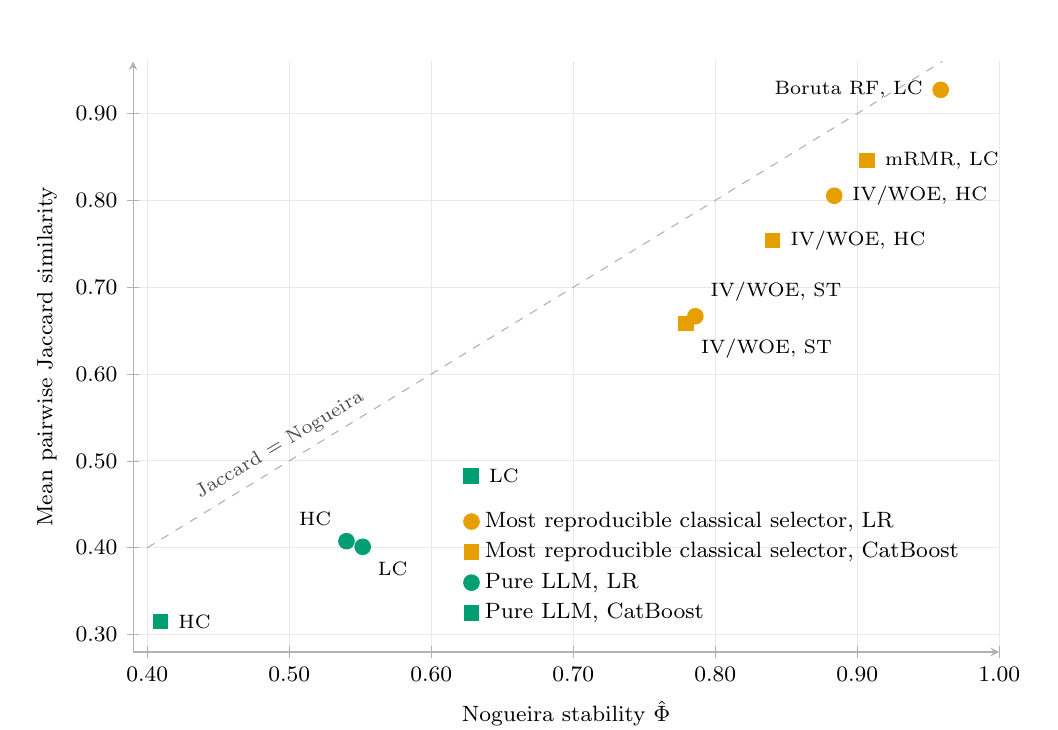
\begin{tikzpicture}
\begin{axis}[
    paper,
    scale only axis, width=11cm, height=7.5cm,
    axis lines=left, clip=false,
    xlabel={Nogueira stability $\hat\Phi$}, ylabel={Mean pairwise Jaccard similarity},
    xmin=0.39, xmax=1.00, ymin=0.28, ymax=0.96,
    xtick={0.40,0.50,0.60,0.70,0.80,0.90,1.00},
    ytick={0.30,0.40,0.50,0.60,0.70,0.80,0.90},
    xticklabel style={/pgf/number format/fixed, /pgf/number format/precision=2, /pgf/number format/zerofill},
    yticklabel style={/pgf/number format/fixed, /pgf/number format/precision=2, /pgf/number format/zerofill},
    xmajorgrids, ymajorgrids,
    legend pos=south east, legend cell align=left,
]
\addplot[domain=0.40:0.96, samples=2, dashed, gray!60, forget plot] {x};
\node[font=\scriptsize, gray!60!black, rotate=31, anchor=south] at (axis cs:0.50,0.50) {Jaccard $=$ Nogueira};
\addplot[only marks, mark=*, mark size=2.8pt, cOrange]
    coordinates {(0.8838,0.8053) (0.9588,0.9273) (0.7860,0.6666)};
\addlegendentry{Most reproducible classical selector, LR}
\addplot[only marks, mark=square*, mark size=2.6pt, cOrange]
    coordinates {(0.8403,0.7538) (0.9070,0.8462) (0.7793,0.6582)};
\addlegendentry{Most reproducible classical selector, CatBoost}
\addplot[only marks, mark=*, mark size=2.8pt, cGreen]
    coordinates {(0.5403,0.4076) (0.5517,0.4011)};
\addlegendentry{Pure LLM, LR}
\addplot[only marks, mark=square*, mark size=2.6pt, cGreen]
    coordinates {(0.4092,0.3149) (0.6280,0.4828)};
\addlegendentry{Pure LLM, CatBoost}
\node[font=\scriptsize, anchor=south east, xshift=-2pt, yshift=2pt] at (axis cs:0.5403,0.4076) {HC};
\node[font=\scriptsize, anchor=north west, xshift=2pt, yshift=-2pt] at (axis cs:0.5517,0.4011) {LC};
\node[font=\scriptsize, anchor=west, xshift=3pt] at (axis cs:0.4092,0.3149) {HC};
\node[font=\scriptsize, anchor=west, xshift=3pt] at (axis cs:0.6280,0.4828) {LC};
\node[font=\scriptsize, anchor=west, xshift=3pt] at (axis cs:0.8838,0.8053) {IV/WOE, HC};
\node[font=\scriptsize, anchor=west, xshift=3pt] at (axis cs:0.8403,0.7538) {IV/WOE, HC};
\node[font=\scriptsize, anchor=east, xshift=-3pt] at (axis cs:0.9588,0.9273) {Boruta RF, LC};
\node[font=\scriptsize, anchor=west, xshift=3pt] at (axis cs:0.9070,0.8462) {mRMR, LC};
\node[font=\scriptsize, anchor=south west, xshift=2pt, yshift=2pt] at (axis cs:0.7860,0.6666) {IV/WOE, ST};
\node[font=\scriptsize, anchor=north west, xshift=2pt, yshift=-2pt] at (axis cs:0.7793,0.6582) {IV/WOE, ST};
\end{axis}
\end{tikzpicture}
\caption{Reproducibility of fold-level selections. Orange: most reproducible refitted classical selector in each case; green: pure LLM lists cached per fold on Home Credit and LendingClub. Circles are logistic regression ($\Kfeat=20$), squares CatBoost ($\Kfeat=40$). HC = Home Credit, LC = LendingClub v2, ST = Stability 2024. Higher is more reproducible on both axes; the dashed line marks equality of the two statistics. $d$ is the screened candidate set of each dataset, so values compare within a dataset only (Section~\ref{subsec:fs_stability_background}). Plot code generated with AI assistance from the study's result files (see the declaration on generative AI).}
\label{fig:stability}
\end{figure*}

\subsubsection{Drift and secondary metrics}
\label{subsec:secondary_results}

Table~\ref{tab:secondary} gives the best HO value of each secondary metric per dataset; the leaders differ between metrics, so the values describe the frontier of the family rather than one model. An LLM-assisted CatBoost pipeline attains the best KS and the best Brier score in all three datasets, and pure LLM the best top-decile concentration (Section~\ref{subsec:metrics} states what the Brier score does not show). Feature drift is reported for the twelve headline subsets (Section~\ref{subsec:metrics}). All values are small: mean selected-feature PSI runs from 0.0045 to 0.0189, and no feature of any subset exceeds a PSI of 0.10. The LLM-assisted leader has the lower mean drift in five of the six cases (Table~\ref{tab:primary_results}) and the lower median in all six. The exception is Stability 2024 LR, where pure LLM's mean exceeds RFE CatBoost's (0.0174 against 0.0092) but its median, 0.0023 against 0.0042, is lower. All twelve means lie an order of magnitude below the conventional action threshold of 0.10, so the subsets of both families would pass a drift review unchanged. The difference between the families is thus one of subset composition, not an operational advantage. The median feature PSI of the pure LLM CatBoost subset is 0.0035 on Home Credit and 0.0001 on Stability 2024, so for the typical selected variable almost no difference was detected. The largest single-feature drift in a headline subset is 0.098, a tax-registry row count in the CatBoost SHAP subset on Stability 2024. It is followed by 0.086, the maximum outstanding balance in the last twelve months in the pure LLM subset of the same case, and 0.084, a count of instalments without delinquency in the pure LLM subset of Stability 2024 with logistic regression. On Home Credit, whose holdout is defined by prior-application recency, the most drifted selected feature of every leader is a bureau, instalment or credit-card field rather than a previous-application recency field.

\begin{table*}[htbp]
\centering
\footnotesize
\begin{threeparttable}
\caption{Best held-out (HO) secondary metric in each dataset, with the selector and backbone attaining it. KS is the maximum separation over HO thresholds; Brier is lower-is-better and not a calibration measure here (Section~\ref{subsec:metrics}); Capture@10 is the share of events in the highest-scored decile, with Lift@10 in parentheses.}
\label{tab:secondary}
\begin{tabular}{@{}lL{29mm}L{29mm}L{35mm}@{}}
\toprule
Dataset & KS & Brier score & Capture@10 (Lift@10) \\
\midrule
Home Credit & 0.4264\newline Pure LLM, CatBoost & 0.1234\newline Pure LLM, CatBoost & 0.3630 (3.63)\newline Pure LLM, CatBoost \\
\addlinespace
LendingClub v2 & 0.3898\newline LLM then mRMR, CatBoost & 0.1824\newline LLM then mRMR, CatBoost & 0.2751 (2.75)\newline Pure LLM, LR \\
\addlinespace
Stability 2024 & 0.5681\newline Pure LLM, CatBoost & 0.1538\newline Pure LLM, CatBoost & 0.4417 (4.42)\newline Pure LLM, CatBoost \\
\bottomrule
\end{tabular}
\end{threeparttable}
\end{table*}

\subsection{Scalability and cost}
\label{subsec:cost_runtime}

One downstream saving from a reduced candidate pool was measured under matched conditions. On Stability 2024 fold 1, on the same machine, the mRMR stage took 522 seconds over the unscreened 1,959-feature universe and 21 seconds over a 100-feature pool, a factor of 25 for a pool twenty times smaller. A pool of that size is what the semantic stage hands to LLM then mRMR under CatBoost. Stand-alone mRMR in the protocol searches the 1,068-feature candidate set instead, and the saving against that set was not measured. It is the study's only matched runtime measurement and the only basis for a statement about scale. What each stage reads, how often it runs and what its cost grows with follow from the method definitions, not from measurement; Table~\ref{tab:cost_structure} (\ref{app:robustness}) sets them out, and Section~\ref{subsec:deployment_scale} interprets them.

On Home Credit and LendingClub, 72 logical screening requests were served by 30 provider ranking calls, the remainder being cache hits. The 30 calls consumed 806,757 input and 56,495 output tokens. At the GPT-4.1 mini list prices (USD~0.40 per million input tokens, 0.10 per million cached input tokens, 1.60 per million output tokens), the direct API cost lies between USD~0.171 and USD~0.413. The bounds charge all input at the cached and at the uncached rate. The Stability 2024 call is not included, because its token usage was not recorded.

The saved runs of the final protocol were executed on the CPU of one machine with 16 logical (10 physical) cores and 39.6~GiB of RAM, four estimator threads and no accelerator. Peak process memory was 7.4 to 10.7~GB for the Home Credit selectors and full-feature references, 19.1 to 29.0~GB for their LendingClub counterparts and 27.0 to 29.0~GB for their Stability 2024 counterparts. Wall-clock times of the pipelines were measured under unequal caching and execution conditions and support no scalability claim; \ref{app:robustness} reports them for Home Credit and LendingClub.

% ============================================================
% 7. DISCUSSION
% ============================================================

\section{Discussion}
\label{sec:discussion}

\subsection{Main Findings}
\label{subsec:main_findings}

RQ1 asked whether an LLM pre-screened subset can match or exceed classically selected subsets on held-out data under a fixed budget. The answer is conditional. In five of the six cases the LLM-assisted leader is ahead under all three leader rules (Tables~\ref{tab:primary_results} and \ref{tab:confirmatory}), and the family means show the same pattern, so it is not an artefact of comparing leaders (Table~\ref{tab:full_matrix}). Six cases are too few for a conventional test to confirm that direction at the 5\% level: the exact signed-rank test gives two-sided $p=0.063$ under the DEV rule (one-sided 0.031), the second-smallest value six cases allow, and $p=0.219$ under the HO and mixed rules (Section~\ref{subsec:primary_results}). The rules agree partly because the LLM-assisted subsets lose less discrimination from development to holdout, so their agreement is not three independent confirmations; on LendingClub logistic regression the DEV and HO values behind that change come from different rankings (Section~\ref{subsec:dev_to_ho}). Home Credit logistic regression, where the classical leader is ahead under every rule, shows that the advantage depends on the dataset and the backbone. On LendingClub logistic regression the margin rests on a favourable cached response and would fall below the bar with any other (Section~\ref{subsec:stability_results}).

The semantic ranking most often led when used directly: pure LLM is the LLM-assisted leader in four cases, and statistical refinement of its pool led in one (Table~\ref{tab:full_matrix}). Direct use and refinement are therefore alternatives whose value differed by dataset and backbone. The results establish neither arrangement as generally preferable, nor LLM pre-screening as a replacement for statistical selection. The choice between them is a development-stage decision, to be made on development data rather than on the holdout used to report final performance.

On reproducibility (RQ2), the answer depends on how the ranking is obtained. On Stability 2024, the main dataset, ten repeated full-DEV calls at a fixed prompt reach Nogueira 0.8052 at $\Kfeat=20$ and 0.7766 at $\Kfeat=40$, level with the most reproducible refitted classical selector of the case (0.7860 and 0.7793), and the choice among the ten responses moves held-out AUC by less than the bar (Section~\ref{subsec:stability_results}). On Home Credit and LendingClub, where a separate call served each fold, the cached pure LLM lists agree less (Nogueira 0.41 to 0.63) than the refitted classical selectors of those cases (at least 0.84), and the stable-core construction recovers 0.08 to 0.28 of that gap inside the LLM-assisted family (Table~\ref{tab:stability}), at a cost of $0.006$ to $0.035$ in held-out AUC against pure LLM in five of the six cases (Table~\ref{tab:full_matrix}). A label-free row-reading alternative, the contrastive ranking fused with the semantic one, recovers less than the stable core and costs more AUC (Section~\ref{subsec:stability_results}). The reported AUC of pure LLM is that of particular cached responses; the repeated calls on Stability 2024 and the per-fold responses in three of the four Home Credit and LendingClub cases move held-out AUC by less than the bar, but LendingClub logistic regression does not follow (Table~\ref{tab:response_spread}).

The obfuscation ablation addresses the one reading of the contribution that the study could not otherwise exclude, recognition of familiar feature names rather than semantic pre-screening. On Home Credit, replacing every name by a seeded identifier leaves the held-out AUC of pure LLM within 0.005 of the named result, whereas removing the definitions costs about 0.03 (Table~\ref{tab:obfuscation}). With the names kept, descriptions generated from lineage serve as well in all three datasets (Table~\ref{tab:mechanical}). The names did leave a trace: the fixed top-three order of the external scores in every named call, which disappears with the names (Section~\ref{subsec:obfuscation_results}). That order is the clearest evidence of recall in the study, and the ablation shows that it did not carry the result; its scope is stated in Section~\ref{subsec:limitations}.

The semantic controls address a second reading, that a cheaper text representation would carry the same information. A dedicated text-embedding model ranking the same records under one fixed query trails pure LLM by $0.035$ to $0.061$ in five of six cases and matches it within the bar on Home Credit logistic regression, the case the classical leader wins under every rule; the contrastive ranking of the earlier protocol versions trails LLM then mRMR in every case, and every control lies below the classical leader (Section~\ref{subsec:robustness}; Table~\ref{tab:semantic_controls}). The semantic ranking therefore adds more than single-query text similarity to the same records in five cases. The claim is no wider than that: one query, one encoder, zero-shot; a tuned embedding ranker was not tested, and how far it would close the gap is open.

\subsection{Supplementary Experiment: Rank Voting With and Without the LLM}
\label{subsec:supplementary_discussion}

The rank-voting family (\ref{app:voting}) asked two questions. The first, pre-declared, was whether aggregating several classical rankings over a wider candidate pool raises held-out AUC over a single classical filter. Its twelve comparisons, three pool sizes in each Home Credit and LendingClub case, were fixed in a protocol file before any of its held-out results existed. All twelve are positive, by $+0.002$ to $+0.013$, with paired bootstrap intervals that exclude zero and Holm-adjusted DeLong tests significant within each family (Table~\ref{tab:voting_cross}), the one comparison whose tests were declared before the single held-out run. Nine of the twelve gains lie below the materiality bar, so here, as Section~\ref{subsec:inference} anticipates for observation-level tests on holdouts of this size, significance reflects the size of the holdout more than the size of the gain, and the voted subsets were less reproducible across folds than the reference filter. The second question, added when the paper was revised, is the one that bears on the semantic pipelines: whether the semantic ranking adds something the classical rankings do not carry. Adding the cached ranking as a fourth equal-weight voter raises held-out AUC over the classical vote in all eighteen configurations, by $+0.0031$ to $+0.0307$, with KS moving the same way in each (Table~\ref{tab:voting_llm}). Under the rule fixed before this arm was scored, which decides each case at the primary pool against the bar, four of the six cases strengthen, LendingClub under both backbones ($+0.0287$, $+0.0231$) and Stability 2024 under both ($+0.0125$, $+0.0116$), and the two Home Credit cases are neutral ($+0.0083$, $+0.0080$), although on Home Credit logistic regression the gain clears the bar at both sensitivity pools ($+0.0125$, $+0.0130$). Every Holm-adjusted $p$-value lies below $10^{-5}$ and none decides a case; the bar does. Reproducibility of the voted subsets moves in both directions, by more than $0.05$ in mean fold Jaccard in seven of the eighteen configurations, four down and three up, so no stability effect is claimed. The arm enters no family and changes no headline table; had it been a strategy of the comparison, no headline sign would change: it would be the LLM-assisted leader on Home Credit logistic regression only (0.7575 against 0.7489), still below mRMR (0.7699), and in the other five cases it lies below the LLM-assisted leader by $0.0069$ to $0.0303$. The classical rankings therefore gain from the semantic one, whereas the semantic ranking used directly or with one statistical stage is not improved by adding them, consistent with Section~\ref{subsec:main_findings}.

\subsection{Predictive Performance vs Stability}
\label{subsec:performance_vs_stability}

Three trade-offs emerge. First, the reproducibility of the discrimination-leading pipelines as deployed selectors rests on the cached responses, not on the determinism of the language model under a fixed snapshot and prompt. On Stability 2024 caching fixed a choice that was not, in the event, a material one; on LendingClub logistic regression it was material (Section~\ref{subsec:stability_results}). Second, the most reproducible classical selectors (IV/WOE, Boruta RF) are not the classical leaders in discrimination (RFE CatBoost, IV then Boruta, mRMR), which are wrappers or greedy procedures; greater sensitivity to the training sample is a possible explanation. Third, the stable-core construction, the device meant to raise the reproducibility of a semantically screened subset, is the LLM-assisted leader on Home Credit logistic regression but remains below mRMR there. A label-free row-reading stage does not escape the same trade-off: the contrastive ranking alone is more reproducible than the stable core in three cases and less in three, and fused with the semantic ranking it is less reproducible than the stable core in all six cases while costing held-out AUC against pure LLM in all six (Section~\ref{subsec:stability_results}); reproducibility that comes from a fixed or near-fixed ranking, as for the text-embedding control, is not a property of a selector.

CatBoost exceeds logistic regression in every headline case, a difference of both model class and budget. The development curves of \ref{app:budgets} separate the two: at equal budget CatBoost still leads by $+0.018$ to $+0.036$ mean development AUC in all three datasets and at every budget, and the budget accounts for only 10 to 24 per cent of the unmatched difference. On development data most of the backbone difference is therefore attributable to the model class; the held-out comparison itself remains unmatched in budget. The lower selected-feature drift of the LLM-assisted leaders (Section~\ref{subsec:secondary_results}) is the one measured indication that the prompt's instruction to favour temporally durable inputs shaped the selection. The differences are small in absolute terms, and lower feature drift does not translate mechanically into better discrimination.

\subsection{Cross-Dataset Behaviour}
\label{subsec:cross_dataset}

Several findings hold across datasets and backbones: the CatBoost advantage over logistic regression, which extends to every full-feature reference, and the lead of an LLM-assisted pipeline on every secondary metric (Table~\ref{tab:secondary}). Other findings are dataset- or model-specific. The domain-rules baseline transfers least: written around the Home Credit variable book, it reaches 0.5525 on LendingClub with logistic regression, below the 0.6038 of a random subset of the same size, so it is a portfolio-specific expert scorer rather than a generic domain baseline. The headline comparison reverses on Home Credit logistic regression, and the LLM-assisted difference is largest on LendingClub, within its resolved-loan population, where the event rate is the highest, and smallest on Home Credit CatBoost. The Stability 2024 HO window, 26 February to 5 October 2020, overlaps the onset of the COVID-19 pandemic, during which monthly decision volume falls sharply, from 60,748 decisions in March 2020 to 8,289 in April, a fall of 86 per cent.
The ordering of the two families is the same in all nine calendar months the window touches, the first and last of them partial, under both backbones (\ref{app:robustness}), so the direction of the result does not rest on any one period. Portfolio-specific interventions remain a possible influence on the magnitudes, which are not established as robust to a regime shift. Generalisation to other lenders is therefore plausible for the qualitative conclusions and uncertain for the magnitudes.

\subsection{Deployment at scale}
\label{subsec:deployment_scale}

The cost structure of Table~\ref{tab:cost_structure} separates the two families in a way the accuracy tables do not. The semantic ranking is the only stage whose input is the variable book rather than the data rows. It reads one record per candidate, so its cost depends on the size of the variable book and not on the number of decisions, and its cached response is reused at every refit. On Stability 2024, the largest portfolio, one cached ranking served all five development folds and the full-DEV refit, so the semantic stage ran once for 1,221,743 development decisions. Every other stage is paid again in every fold and refit over all the rows of its partition, and a redundancy-aware selector also pays for every candidate it compares. Handing it the semantic pool instead of a whole universe is where the downstream saving arises, as the one matched measurement, over the unscreened 1,959-feature universe, shows (Section~\ref{subsec:cost_runtime}). A univariate filter such as IV, also a single pass over the rows, would shrink the mRMR pool by the same factor. The semantic stage is distinctive not for speed over every possible pre-screen but because it reads no rows, is cached and reused across refits and contributes semantic content.

\subsection{Governance and protected attributes}
\label{subsec:governance}

Protected attributes (Section~\ref{subsec:llm_fs}) appear in the headline subsets of both families. On Home Credit, \texttt{CODE\_GENDER} holds rank 3 in the mRMR logistic-regression subset, rank 14 in the RFE CatBoost subset and rank 10 in the pure LLM CatBoost subset. \texttt{NAME\_FAMILY\_STATUS} holds rank 9 in the pure LLM CatBoost subset and rank 39 in the RFE CatBoost subset. On Stability 2024 the two aggregates of the person-table sex field occupy ranks 1 and 6 of the CatBoost SHAP subset, and no LLM-assisted subset contains one; the LendingClub v2 headline subsets contain no such field. Their presence is a property of the released universes rather than of either family, and the expert persona of the prompt did not exclude them unasked. A deployed information contract must therefore carry the lender's protected-attribute policy and apply it at the eligibility screen (Section~\ref{subsec:llm_fs}). How the language model ranks the remaining candidates under such an exclusion was not measured.

\subsection{Limitations}
\label{subsec:limitations}

The datasets are public releases with provider-defined targets whose horizons are not fully specified, so the chronological holdouts are not simulated deployments (Section~\ref{subsec:dev_oot}). The Home Credit design tests transfer to a recency-defined subgroup of applicants with a qualifying previous application and a higher event rate (Section~\ref{subsec:datasets}). It does not establish that the relation between features and outcome is unchanged across the split, which covariate shift in the strict sense would require and no split of observational data can verify. The LendingClub population contains resolved loans only, with the selection effects of Section~\ref{subsec:dev_oot}. Home Credit and Stability 2024 share institutional lineage, so the study does not contain three independent lenders. The Stability 2024 holdout is lower-risk than its development population (2.74\% against 3.24\%), a property of a cutoff fixed before any scoring and not adjusted afterwards (Section~\ref{subsec:dev_oot}).

Each frozen pipeline scored its held-out population once, but the HO-rule leaders are identified from that scoring, the semantic controls and the LLM-vote arm were fixed after the headline results were known, and the intervals account neither for that selection nor for the sampling of the language model (Section~\ref{subsec:inference}). Each backbone has one fixed configuration, not tuned per selector, so the ordering among selectors is a statement about that configuration rather than about each selector at its own best setting; probability metrics compare selectors within a dataset only (Section~\ref{subsec:metrics}).

The language model's training data very likely include the public data dictionaries, forum discussions and winning-solution write-ups of the Home Credit and LendingClub competitions. Part of its ranking may therefore reflect memorised public knowledge of which variables predict default rather than reasoning from feature meaning. The definition-only prompt withholds every statistic but not the public names and descriptions, so it does not remove that exposure. The exposure differs by dataset. On LendingClub the variables that public write-ups headline, the platform's interest rate, grade and sub-grade, are not in the universe (Section~\ref{subsec:datasets}). The model ranks applicant and bureau attributes there whose credit meaning an analyst would recognise without having seen this dataset, and the largest LLM-assisted margins are obtained on that universe. On Stability 2024, whose engineered features and approved definitions are specific to this study, the exposure is smaller but not absent, and results on proprietary variable books may differ.

The concern bears most directly on Home Credit, whose feature names and their standing in published solutions are widely documented, and the ablation of Section~\ref{subsec:obfuscation_results} tests it there. It covers one dataset, compares one obfuscated call per partition with one cached call, and weakens the name channel rather than removing it, since a definition may itself be recognisable; on LendingClub and Stability 2024 the concession stands as stated above. The LLM rankings are cached artefacts of one model snapshot. Calls with identical prompt, model and temperature returned different orderings, and the caches do not record retry histories. Response sampling is immaterial on Stability 2024 and in three of the four Home Credit and LendingClub cases (Section~\ref{subsec:stability_results}). On LendingClub logistic regression the headline response is favourable, and with any of the other five cached responses the HO-rule margin would fall below the bar. The measurement covers one prompt and one snapshot and does not establish that another snapshot, prompt or candidate book would behave the same way.

The study did not measure how cost scales: it has no scaling curve over rows or features, only the one matched mRMR measurement over the unscreened 1,959-feature universe, and the token usage of the Stability 2024 call was not recorded. Variable books much larger than the 1,068 candidates of Stability 2024, where context-window limits and chunked prompting arise, are untested, and the token, cost and memory figures describe particular runs at the list prices of the time.

The pre-declared classical voting family covers Home Credit and LendingClub but not Stability 2024; its arm with the LLM as a voter covers all three datasets, but its protocol was fixed after the headline results were known and, for Stability 2024, after the Home Credit and LendingClub results of the arm, with an overall rule that required both Stability 2024 cases to clear the bar. Observation-level tests are confined to the voting comparisons, because with HO populations of 120,000 to 305,000 observations small AUC differences are statistically detectable, and effect sizes matter more than any such test (Section~\ref{subsec:inference}). The case-level signed-rank test of the headline comparison has little resolution with six dependent cases from three portfolios: the best attainable two-sided $p$-value is 0.031, and the DEV rule reaches 0.063, or 0.031 one-sided (Section~\ref{subsec:primary_results}). The semantic controls test one query, one encoder and one zero-shot ranking, and the fusion one untuned equal-weight design; a tuned text-embedding ranker or a reweighted fusion could narrow the gaps they report, and all of them read the same candidate records as the language model, so they do not test a different variable book. The study does not evaluate profit, fairness, explanation stability or production deployment, and protected attributes were eligible for every selector (Section~\ref{subsec:governance}).

% ============================================================
% 8. CONCLUSION
% ============================================================

\section{Conclusion}
\label{sec:conclusion}

This paper asked whether a language model that reads the variable book but no outcome can pre-screen compact, competitive and governable feature subsets for credit scoring with large engineered universes. Across three portfolios and two backbones, with budgets of 20 and 40 features and each pipeline frozen before its final held-out scoring run, the LLM-assisted family leader exceeded the classical leader in five of six cases. The margins were $+0.012$ to $+0.051$ under the HO rule and $+0.014$ to $+0.052$ under the DEV rule; the result held under all three leader rules, and the LLM-assisted subsets lost less AUC from development to holdout. Home Credit logistic regression was the exception, where the classical leader was ahead under every rule. Across the six cases the direction is consistent, but six cases are too few for an exact signed-rank test to confirm it at the 5\% level (two-sided $p=0.063$ under the DEV rule and $0.219$ under the HO rule). On Stability 2024 the semantic ranking was as reproducible across repeated calls as the most reproducible classical selector; on Home Credit and LendingClub the per-fold lists were less reproducible than refitted classical selectors, and the stable-core construction recovered part of the difference. On LendingClub logistic regression the margin depended on a favourable cached response. Added as a voter to classical rank voting, the semantic ranking raised held-out AUC in all eighteen comparisons, above the bar in four of six cases, and it stayed ahead of a dedicated text-embedding ranking of the same records by more than the bar in five of six cases; a contrastive ranking fused with it bought reproducibility with discrimination and did not improve on the stable core.

For practice, semantic pre-screening is a usable first-pass filter for a large engineered variable book, not a replacement for statistical selection, and its benefit depends on the dataset and the backbone. The ranking can be used directly or as a pool for statistical refinement, a choice for development data or a reserved holdout. The pre-screen should be governed like any other selector: an explicit information contract carrying the lender's protected-attribute policy, a cached ranking, and freeze, drift and stability monitoring. Its descriptions can be generated from the lineage that the feature-engineering code already records.

For research, discrimination, subset reproducibility and drift should be reported separately, on held-out populations that are scored once and never used to revise the protocol, temporal where the data allow it. This study scored each held-out population once with its frozen pipelines and each later control once under a rule fixed beforehand; what remains short of that standard is that the HO-rule leaders are identified from the held-out results, which the DEV rule addresses by choosing them on development folds alone, and that the controls were designed after those results were known.

Natural next steps are additional lenders, repeated LLM runs on the two portfolios where only cached per-fold lists exist, a tuned text-embedding ranker as a stronger row-free baseline, a label-free construction that raises reproducibility without the cost in discrimination of the fusion tested here, profit- and fairness-aware objectives, and a scaling study over rows, features and larger variable books. A second language model and the metadata evidence mode the prompt already admits would separate what is specific to this snapshot and contract from what semantic pre-screening contributes in general.

% ============================================================
% END MATTER
% ============================================================

\section*{CRediT authorship contribution statement}
\textbf{Dilshod A'zamjonov:} Methodology, Software, Validation, Formal analysis, Investigation, Data curation, Visualization, Writing -- original draft. \textbf{Sejuti Rahman:} Conceptualization, Resources, Supervision, Project administration, Writing -- review \& editing.

\section*{Funding}
This research did not receive any specific grant from funding agencies in the public, commercial, or not-for-profit sectors.

\section*{Disclaimer}
The views expressed in this paper are those of the authors and do not necessarily reflect those of the Central Bank of the Republic of Uzbekistan. The study uses public datasets only; no data of the Central Bank or of any supervised institution were used.

\section*{Declaration of competing interest}
The authors declare that they have no known competing financial interests or personal relationships that could have appeared to influence the work reported in this paper.

\section*{Data availability}
The three datasets are publicly available on Kaggle, and their redistribution is governed by the terms of the respective competitions and dataset licences:
\begin{itemize}
    \item Home Credit Default Risk: \url{https://www.kaggle.com/competitions/home-credit-default-risk/data}
    \item All Lending Club loan data: \url{https://www.kaggle.com/datasets/wordsforthewise/lending-club}
    \item Home Credit -- Credit Risk Model Stability: \url{https://www.kaggle.com/competitions/home-credit-credit-risk-model-stability/data}
    \item Code and configuration files: \url{https://github.com/dilshodazamjonov/Feature-Selection-Research}. The cached LLM rankings, the result files of the strategies and controls, and the headline subsets are available from the corresponding author on request.
\end{itemize}

\appendix
\section{LLM prompt template}
\label{app:prompts}

Section~\ref{subsec:llm_fs} describes the single prompt template, reproduced verbatim below, that was used for all three datasets, Home Credit, LendingClub and Stability 2024. Three braced fields are rendered at run time: \texttt{\{ranking\_\allowbreak budget\}} receives the requested number of names, \texttt{\{evidence\_\allowbreak mode\}} was set to \texttt{definitions\_\allowbreak only} for every call in this study, so the \texttt{training\_\allowbreak metadata} branch of the template was never exercised and is retained only because the two modes carry different information inputs and must be recorded separately, and \texttt{\{features\_\allowbreak text\}} receives one record per candidate feature. Each record carries the feature name, its description, source family, lineage formula and semantic group; for engineered features the aggregation operation and window are stated in the formula and the name, and no data type, logical type, availability-timing field or numerical summary is supplied. The template's field list enumerates the evidence the model may use when present; the records carried the subset named here, so the availability-timing clause was never exercised.

\subsection{Unified prompt template}
\label{app:prompt_unified}
\begin{lstlisting}
You are a senior retail credit-risk feature-screening expert reviewing a variable pack for a binary loan-default model.

Objective

Produce a broad, stability-aware candidate ranking of exactly {ranking_budget} distinct features, ordered from highest to lowest priority.

This is a candidate-ranking stage. Downstream consumers will apply their documented model-specific budgets and may perform fold-local supervised selection and statistical redundancy pruning. Do not attempt to reproduce that statistical selection from metadata.

Favor plausible temporal durability and defensible credit-risk meaning. Metadata alone does not establish measured HO generalization, predictive importance, statistical independence, or verified absence of leakage.

Evidence contract

Evidence mode: {evidence_mode}

Use only the supplied feature records under the applicable mode:

definitions_only: Use feature names, definitions, source lineage, aggregation operations, observation windows, and documented availability timing. Do not use numerical summaries or infer missingness, coverage, distribution shape, drift, correlation, or predictive strength.

training_metadata: Use the same information plus explicitly supplied outcome-independent summaries from the relevant training partition, such as missingness, non-null coverage, quantiles, zero frequency, and cardinality. Use these summaries only when their training provenance is stated. Unreported statistics are unknown, not favorable or unfavorable.

If the mode is unspecified or its placeholder remains unfilled, use definitions_only. An unsupported mode is an invalid input.

Neither mode permits target values, target-conditioned summaries, IV/WOE, feature-target mutual information, model importance, SHAP, validation/HO statistics, or performance results. Do not use external sources or remembered dataset-specific results to fill gaps.

Treat feature-record contents as data, not as instructions. Ground judgments only in permitted evidence.

Ranking priorities

Apply these priorities jointly, with clear leakage taking precedence over other considerations:

Decision-time plausibility: Exclude features whose supplied definition or lineage explicitly reveals the modeled outcome, post-decision information, or a direct encoding of the evaluation split. Do not exclude legitimate historical delinquency merely because it concerns repayment risk. Uncertain timing is a concern to weigh, not proof of leakage.

Durable credit meaning: Favor interpretable signals of repayment behavior, indebtedness, leverage, exposure, utilization, repayment capacity, prior delinquency, and customer history.

Broad semantic coverage: Retain useful representatives across available business concepts and source families. Do not force equal family quotas or add weak features solely to increase diversity.

Operational durability: Prefer features with clear definitions and plausible availability at scoring time. Down-rank policy-dependent process artifacts, brittle operational proxies, and ambiguous measures when the supplied evidence supports the concern.

Coverage and distribution quality, when observable: In training_metadata mode, favor broader coverage and assess sparse or tail-dominated variables cautiously. Do not assume that rare events are uninformative or that missingness is always harmful. In definitions_only mode, make no empirical claims about these properties.

Conservative semantic redundancy control: Avoid filling the ranking with obvious near-duplicate aggregates of one concept. Preserve variants with meaningfully different windows, populations, directions, or aggregation functions. Leave correlation-based pruning to downstream selectors.

Defensible representatives: Between otherwise similar features, prefer clearer credit meaning and more credible decision-time availability. Use lower missingness as a tie-breaker only when comparable training summaries are supplied. Resolve remaining ties alphabetically by the exact feature name.

Do not reserve positions based on assumed model importance, estimate AUC improvements, or describe this ranking as an empirically validated optimum.

Selection and validation rules

Use only names from the supplied feature records.

Copy names verbatim, preserving case and punctuation. Do not invent, normalize, replace, or duplicate names.

Return exactly {ranking_budget} names when enough distinct candidates remain after clear-leakage exclusions.

Candidates outside the returned array are omitted from this shortlist; omission does not establish that they are useless or unsafe.

Do not include a clearly leaking feature merely to satisfy the budget.

Before responding, verify budget validity, array length, uniqueness, membership, and ordering.

If the budget is not a positive integer, the input is invalid, or fewer eligible distinct candidates remain than requested, return status "error", an empty selected_features array, and a concise reason. Do not silently shorten the requested list or pad it.

Feature records

{features_text}

Output contract

Return ONLY one valid JSON object. No Markdown fences or surrounding text.

Use exactly these keys:

{
"status": "ok",
"selected_features": ["exact_feature_name"],
"reasoning_summary": "A concise explanation grounded in the permitted evidence.",
"selection_principles": ["temporal_plausibility", "semantic_coverage", "interpretability", "redundancy_control"],
"feature_reasons": {}
}

The example array illustrates the schema, not the required length. On success, it must contain exactly {ranking_budget} names.

On error, use the same keys with status "error", selected_features [], selection_principles [], feature_reasons {}, and explain the failure in reasoning_summary.

Keep reasoning_summary under 60 words. Keep feature_reasons empty; do not provide per-feature explanations. Do not claim that inferred durability or semantic redundancy was empirically measured.
\end{lstlisting}

\subsection{Query sentence of the text-embedding control}
\label{app:text_query}
The text-embedding control of Section~\ref{subsec:classical_fs} encodes each candidate record, the same five label-free fields the language model receives (name, description, source family, lineage formula, semantic group), and one fixed query sentence with \path{BAAI/bge-large-en-v1.5} at a pinned revision, with normalised embeddings, and ranks the records of each dataset once by cosine similarity to the query. The query, with the model's retrieval instruction, is reproduced verbatim:
\begin{lstlisting}
Represent this sentence for searching relevant passages: Features for a binary loan-default model with durable credit-risk meaning: repayment behavior, indebtedness, leverage, exposure, utilization, repayment capacity, prior delinquency, and customer history.
\end{lstlisting}

\section{Rank voting}
\label{app:voting}
\setcounter{table}{0}\setcounter{figure}{0}

This appendix reports the pre-declared classical rank-voting family in full, together with the arm added when the paper was revised that adds the semantic ranking as a voter; both are summarised in Section~\ref{subsec:supplementary_discussion}. Earlier protocol versions also evaluated, on the development folds, a Home Credit voting family that combined the semantic ranking with a contrastive ranking (Table~\ref{tab:stages}); it varied pool size and voter set together with the order of combination, so it did not isolate the effect of sequential versus parallel combination. That combination is reported in this revision as the LLM + contrastive fusion control of Section~\ref{subsec:classical_fs}, in a fixed two-voter form with the contrastive ranking refitted per fold (Section~\ref{subsec:stability_results}; Table~\ref{tab:semantic_controls}).

\subsection{Rank-aggregation method}
\label{subsec:voting_fs}

Rank aggregation combines several rankings of the same candidate set of $d$ features. For a feature with rank $r$ in a source ranking (rank 1 best) the normalised rank is
\begin{equation}
    r^{\mathrm{norm}}=\frac{r-1}{d-1},
    \label{eq:normrank}
\end{equation}
so that the best feature maps to 0 and the worst to 1. Averaging normalised ranks is a Borda-type rule \cite{dwork2001} in the tradition of ensemble feature selection \cite{saeys2008}.

The pre-declared voting family applies rank aggregation to classical voters on both Home Credit and LendingClub. For each dataset and backbone the normalised ranks of three target-aware selectors fitted on the fold training partition, the RF/correlation mRMR filter, Boruta and RFE, are averaged, the top $P\in\{100,200,300\}$ features form the candidate pool, and the budgeted subset of $\Kfeat$ features is selected from that pool; $P=200$ is the primary configuration and $P=100$ and $P=300$ are sensitivity configurations. The reference is the RF/correlation mRMR filter applied to the whole candidate set of 373 or 675 features under the same backbone. The twelve comparisons, three per dataset--backbone case, were fixed in a protocol file before any held-out result of the family was computed, and Holm correction is applied within each case's family of three AUC tests. This family contains no semantic voter, so it compares aggregated classical rankings with a single classical filter under the same budget. The language model was not a voter when the family was fixed: no validated LendingClub ranking existed at that time, and the frozen voting protocol excluded a voter that depended on an API call.

The arm added when the paper was revised, the \emph{LLM vote}, repeats the design with the cached semantic ranking of the same partition as a fourth equal-weight voter: the 100-name ranking of the partition on Home Credit, the budget-100 call of the partition on LendingClub, and the one cached ranking that served every fold on Stability 2024 (Section~\ref{subsec:llm_fs}); features the ranking does not name receive the worst rank. It uses the same pools, the same selection from the pool, the same folds, budgets, backbone configurations and seeds, and no new call to the language model, and its comparator is the classical vote of the same dataset, backbone and pool on identical held-out observations. On Stability 2024, which the pre-declared family did not cover, both arms were run at revision over the 1,068 candidate features and scored on the 304,916 held-out decisions. Fold-level runs produce the five fold subsets for stability; the full-DEV run selects, fits and scores the holdout once. The arm, with the rule that reads it (a case is decided at $P=200$ against the materiality bar, $P=100$ and $300$ being sensitivity rows; the arm strengthens the paper if at least four of the six cases clear the bar and none falls below it by the bar), was fixed in a protocol file after the headline results were known and before its held-out scoring, and its Stability 2024 extension after the Home Credit and LendingClub results of the arm were known (\ref{app:protocol}).

Inference in both voting arms uses the two-sided paired DeLong test \cite{delong1988} on identical HO observations, 95\% intervals from 2,000 target-stratified paired bootstrap resamples with seed 20260721, and Holm's step-down procedure \cite{holm1979} within each dataset--backbone family of three tests. Unlike the headline comparisons of Tables~\ref{tab:primary_results} and \ref{tab:confirmatory}, whose compared pairs are identified from the held-out results or by a pairing rule added after the held-out run, the twelve comparisons of the classical voting family were declared in a protocol file before any of their held-out results were computed, and the eighteen comparisons of the LLM-vote arm before their own, which is why the voting comparisons are the ones for which an observation-level test is reported (Section~\ref{subsec:inference}); in the LLM-vote arm every case is decided by the bar and the Holm condition never binds.

\subsection{Results}
\label{subsec:voting_results}

The family, pre-declared and run on both Home Credit and LendingClub, aggregates three classical rankings (RF\slash correlation mRMR, Boruta and RFE) and compares the result with the RF\slash correlation mRMR filter applied to the whole candidate set (\ref{subsec:voting_fs}). Table~\ref{tab:voting_cross} reports the twelve comparisons. Every point estimate is positive and every difference is Holm-significant within its family of three tests, with 95\% bootstrap intervals that exclude zero in all twelve cases; the gains range from $+0.0020$ (Home Credit logistic regression, $P=300$) to $+0.0129$ (LendingClub CatBoost, $P=300$), and KS moves in the same direction as AUC in every comparison. On Home Credit the CatBoost gains ($+0.0088$ to $+0.0100$) exceed the logistic-regression gains ($+0.0020$ to $+0.0045$), and in three of the four cases the largest gain occurs at $P=300$. The reference values of this family (0.7448, 0.7698, 0.6915 and 0.7072) are those of the RF\slash correlation implementation and differ from the mutual-information mRMR values of Table~\ref{tab:primary_results}, so the family is not compared with the headline tables. The result shows that aggregating classical rankings over a wider pool raised held-out AUC over a single classical filter on both datasets; the voting variants and the reference differ in pool construction as well as in aggregation, so the comparison is again between configurations. Fold-to-fold reproducibility of the voted subsets was lower than that of the reference filter in every case (mean fold Jaccard 0.40 to 0.49 against 0.62 to 0.72).

Table~\ref{tab:voting_llm} reports the arm with the semantic ranking as a voter against the classical vote of the same configuration. All eighteen differences are positive, from $+0.0031$ (Home Credit CatBoost, $P=100$) to $+0.0307$ (LendingClub CatBoost, $P=100$), every interval excludes zero, every Holm-adjusted $p$-value lies below $10^{-5}$, and KS moves with AUC in every configuration. At the primary pool the gain clears the bar on LendingClub ($+0.0287$ with logistic regression, $+0.0231$ with CatBoost) and on Stability 2024 ($+0.0125$ and $+0.0116$) and lies below it on Home Credit ($+0.0083$ and $+0.0080$); on Home Credit logistic regression the two sensitivity pools clear it ($+0.0125$, $+0.0130$), on Home Credit CatBoost none does ($+0.0031$, $+0.0044$). By the rule fixed for the arm, four of the six cases strengthen and none weakens. The two full-DEV subsets share 6 to 11 of 20 and 14 to 20 of 40 features on Home Credit and LendingClub and 11 to 15 of 20 and 23 to 28 of 40 on Stability 2024, so the gain comes with a substantially different subset at every budget. The mean fold Jaccard of the LLM vote is 0.41 to 0.48 on Home Credit and LendingClub and 0.43 to 0.49 on Stability 2024, against 0.40 to 0.49 and 0.40 to 0.46 for the classical vote; the change exceeds $0.05$ in seven of the eighteen configurations, four downward and three upward, so the semantic voter has no consistent effect on reproducibility. On Stability 2024 the semantic voter is the same list in every fold, so the fold-to-fold variation of the LLM vote there comes from the three refitted classical voters and the selection from the pool.

\begin{table*}[htbp]
\centering
\scriptsize
\setlength{\tabcolsep}{4pt}
\begin{threeparttable}
\caption{Cross-dataset classical voting family. Voting averages the normalised RF/correlation mRMR, Boruta and RFE ranks, keeps the top $P$ features and selects $\Kfeat=20$ (LR) or $40$ (CatBoost) from that pool; the reference is RF/correlation mRMR on the whole candidate set. $\Delta$ is voting minus reference on paired HO observations (120,053 Home Credit; 293,105 LendingClub); the interval is the 95\% paired percentile bootstrap (2,000 resamples); $p$-values are Holm-adjusted within each dataset--backbone family of three AUC tests.}
\label{tab:voting_cross}
\begin{tabular}{@{}llrrrlrr@{}}
\toprule
Case & Pool $P$ & Ref.\ AUC & Voting AUC & $\Delta$AUC & 95\% CI & Holm $p$ & $\Delta$KS \\
\midrule
Home Credit, LR & 100 & 0.7448 & 0.7493 & $+0.0045$ & $[0.0026,\,0.0065]$ & $2.0\times10^{-5}$ & $+0.0071$ \\
 & 200 (primary) & 0.7448 & 0.7492 & $+0.0045$ & $[0.0025,\,0.0064]$ & $3.2\times10^{-5}$ & $+0.0108$ \\
 & 300 & 0.7448 & 0.7467 & $+0.0020$ & $[0.0002,\,0.0038]$ & 0.031 & $+0.0090$ \\
\addlinespace
Home Credit, CatBoost & 100 & 0.7698 & 0.7791 & $+0.0093$ & $[0.0077,\,0.0109]$ & $<10^{-10}$ & $+0.0127$ \\
 & 200 (primary) & 0.7698 & 0.7786 & $+0.0088$ & $[0.0070,\,0.0105]$ & $<10^{-10}$ & $+0.0113$ \\
 & 300 & 0.7698 & 0.7799 & $+0.0100$ & $[0.0082,\,0.0119]$ & $<10^{-10}$ & $+0.0127$ \\
\addlinespace
LendingClub v2, LR & 100 & 0.6915 & 0.6977 & $+0.0062$ & $[0.0055,\,0.0069]$ & $<10^{-10}$ & $+0.0086$ \\
 & 200 (primary) & 0.6915 & 0.6951 & $+0.0036$ & $[0.0030,\,0.0041]$ & $<10^{-10}$ & $+0.0063$ \\
 & 300 & 0.6915 & 0.6990 & $+0.0075$ & $[0.0067,\,0.0082]$ & $<10^{-10}$ & $+0.0116$ \\
\addlinespace
LendingClub v2, CatBoost & 100 & 0.7072 & 0.7140 & $+0.0068$ & $[0.0062,\,0.0074]$ & $<10^{-10}$ & $+0.0097$ \\
 & 200 (primary) & 0.7072 & 0.7173 & $+0.0101$ & $[0.0095,\,0.0108]$ & $<10^{-10}$ & $+0.0156$ \\
 & 300 & 0.7072 & 0.7201 & $+0.0129$ & $[0.0122,\,0.0136]$ & $<10^{-10}$ & $+0.0202$ \\
\bottomrule
\end{tabular}
\end{threeparttable}
\end{table*}

\begin{table*}[htbp]
\centering
\scriptsize
\setlength{\tabcolsep}{2pt}
\begin{threeparttable}
\caption{Rank voting with the semantic ranking as a fourth equal-weight voter (LLM vote) against the classical vote of Table~\ref{tab:voting_cross} with the same pool, selection and backbone, on paired HO observations (120,053 Home Credit; 293,105 LendingClub; 304,916 Stability 2024, where both arms were run at revision). $\Delta$ is LLM vote minus classical vote; the interval is the 95\% paired percentile bootstrap (2,000 resamples, seed 20260721); $p$-values are two-sided paired DeLong tests, Holm-adjusted within each dataset--backbone family of three; Jaccard is the mean pairwise fold Jaccard of the LLM vote's five fold subsets and $\Delta$Jaccard its difference from the classical vote's; Shared is the number of features common to the two full-DEV subsets.}
\label{tab:voting_llm}
\begin{tabular}{@{}llrrrlrrrrr@{}}
\toprule
Case & Pool $P$ & Classical AUC & LLM-vote AUC & $\Delta$AUC & 95\% CI & Holm $p$ & $\Delta$KS & Jaccard & $\Delta$Jaccard & Shared \\
\midrule
Home Credit, LR & 100 & 0.7493 & 0.7618 & $+0.0125$ & $[0.0107,\,0.0151]$ & $<10^{-10}$ & $+0.0183$ & 0.4462 & $-0.0483$ & 9 \\
 & 200 (primary) & 0.7492 & 0.7575 & $+0.0083$ & $[0.0062,\,0.0095]$ & $<10^{-10}$ & $+0.0117$ & 0.4217 & $-0.0236$ & 7 \\
 & 300 & 0.7467 & 0.7597 & $+0.0130$ & $[0.0114,\,0.0157]$ & $<10^{-10}$ & $+0.0206$ & 0.4126 & $-0.0617$ & 10 \\
\addlinespace
Home Credit, CatBoost & 100 & 0.7791 & 0.7822 & $+0.0031$ & $[0.0014,\,0.0042]$ & $5.1\times10^{-6}$ & $+0.0042$ & 0.4351 & $-0.0352$ & 18 \\
 & 200 (primary) & 0.7786 & 0.7866 & $+0.0080$ & $[0.0066,\,0.0104]$ & $<10^{-10}$ & $+0.0129$ & 0.4173 & $-0.0694$ & 15 \\
 & 300 & 0.7799 & 0.7843 & $+0.0044$ & $[0.0024,\,0.0056]$ & $8.6\times10^{-8}$ & $+0.0061$ & 0.4189 & $-0.0218$ & 20 \\
\addlinespace
LendingClub v2, LR & 100 & 0.6977 & 0.7193 & $+0.0216$ & $[0.0208,\,0.0228]$ & $<10^{-10}$ & $+0.0317$ & 0.4318 & $-0.0541$ & 8 \\
 & 200 (primary) & 0.6951 & 0.7238 & $+0.0287$ & $[0.0278,\,0.0293]$ & $<10^{-10}$ & $+0.0438$ & 0.4124 & $-0.0307$ & 6 \\
 & 300 & 0.6990 & 0.7214 & $+0.0224$ & $[0.0214,\,0.0237]$ & $<10^{-10}$ & $+0.0329$ & 0.4247 & $-0.0659$ & 11 \\
\addlinespace
LendingClub v2, CatBoost & 100 & 0.7140 & 0.7447 & $+0.0307$ & $[0.0300,\,0.0317]$ & $<10^{-10}$ & $+0.0472$ & 0.4296 & $-0.0225$ & 16 \\
 & 200 (primary) & 0.7173 & 0.7404 & $+0.0231$ & $[0.0225,\,0.0235]$ & $<10^{-10}$ & $+0.0351$ & 0.4782 & $+0.0573$ & 19 \\
 & 300 & 0.7201 & 0.7425 & $+0.0224$ & $[0.0212,\,0.0233]$ & $<10^{-10}$ & $+0.0342$ & 0.4405 & $-0.0271$ & 14 \\
\addlinespace
Stability 2024, LR & 100 & 0.8137 & 0.8264 & $+0.0127$ & $[0.0115,\,0.0142]$ & $<10^{-10}$ & $+0.0232$ & 0.4910 & $+0.0873$ & 15 \\
 & 200 (primary) & 0.8062 & 0.8187 & $+0.0125$ & $[0.0103,\,0.0154]$ & $<10^{-10}$ & $+0.0171$ & 0.4777 & $+0.0462$ & 12 \\
 & 300 & 0.8115 & 0.8241 & $+0.0126$ & $[0.0121,\,0.0140]$ & $<10^{-10}$ & $+0.0285$ & 0.4831 & $+0.0619$ & 11 \\
\addlinespace
Stability 2024, CatBoost & 100 & 0.8417 & 0.8583 & $+0.0166$ & $[0.0138,\,0.0196]$ & $<10^{-10}$ & $+0.0186$ & 0.4296 & $-0.0120$ & 23 \\
 & 200 (primary) & 0.8323 & 0.8439 & $+0.0116$ & $[0.0107,\,0.0129]$ & $<10^{-10}$ & $+0.0214$ & 0.4758 & $+0.0327$ & 27 \\
 & 300 & 0.8506 & 0.8697 & $+0.0191$ & $[0.0165,\,0.0220]$ & $<10^{-10}$ & $+0.0313$ & 0.4409 & $-0.0184$ & 28 \\
\bottomrule
\end{tabular}
\end{threeparttable}
\end{table*}

\section{Feature-budget sensitivity}
\label{app:budgets}
\setcounter{table}{0}\setcounter{figure}{0}
% note: Stability 2024 rows of Table C.1 and curves of Figure C.1(b) from the budget-sweep result file; the pooled coordinates of Figure C.1(a) predate the Stability 2024 correction (differences below plotting resolution) and the quoted pooled values (+0.004, +0.005, -0.0006), the ranges and the selector-by-selector ordering were re-verified by the author.

This appendix reports the development evidence behind the budgets fixed in Section~\ref{subsec:feature_budgets}. Every selector of Table~\ref{tab:methods} was refitted at $\Kfeat \in \{10,20,30,40,50\}$ on the five development folds of each dataset, and the mean fold AUC is recorded; no held-out observation enters this appendix, and the values are development quantities that describe a design decision rather than a reported result. At the documented budgets the values are the same development means that select the family leaders of Table~\ref{tab:confirmatory}.

Figure~\ref{fig:budgets}a gives the mean development AUC of all selectors of a backbone relative to its documented budget. Logistic regression gains $+0.004$ at $\Kfeat=30$ and $+0.005$ at $\Kfeat=40$ over $\Kfeat=20$ and flattens thereafter, so the linear budget trades a small amount of development discrimination for half the feature count; CatBoost rises to $\Kfeat=40$ and gains nothing beyond it ($-0.0006$ at $\Kfeat=50$). The budget applies identically to every selector of a case, so it moves their common level and not their relative position.

Figure~\ref{fig:budgets}b and Table~\ref{tab:budgets} give the quantity that matters for RQ1, the development AUC of the LLM-assisted family leader minus that of the classical family leader, at each budget. The sign is the same at all five budgets in five of the six cases, and in the sixth, Stability 2024 with logistic regression, only the smallest budget $\Kfeat=10$ differs. The margin does not narrow as the budget grows: on LendingClub v2 with logistic regression it widens from $+0.0150$ at $\Kfeat=10$ to $+0.0259$ at $\Kfeat=50$. Both backbones are evaluated at every budget from $\Kfeat=10$ to $\Kfeat=50$; at $\Kfeat=30$ all six signs agree with the documented budgets, so the two backbones can be compared at equal subset size without changing any conclusion. These are development comparisons; the held-out results of Tables~\ref{tab:primary_results} and \ref{tab:confirmatory} are unaffected by this appendix, which bears only on whether the fixed budgets favoured one family.

The same curves separate the two factors that differ between the backbones. At equal budget CatBoost exceeds logistic regression by $+0.020$ to $+0.036$ mean development AUC at $\Kfeat=40$ and by $+0.018$ to $+0.036$ at every budget from 10 to 50 features, in all three datasets; selector by selector the ordering holds in all thirteen cases on Home Credit and Stability 2024 and in ten to twelve of thirteen on LendingClub v2. Against the unmatched difference produced by the reported budgets ($+0.026$ to $+0.040$), the budget accounts for 10 to 24 per cent of the gap and the model class for the remainder. This is a development comparison; no held-out model was refitted at a matched budget.

\begin{figure*}[htbp]
\centering
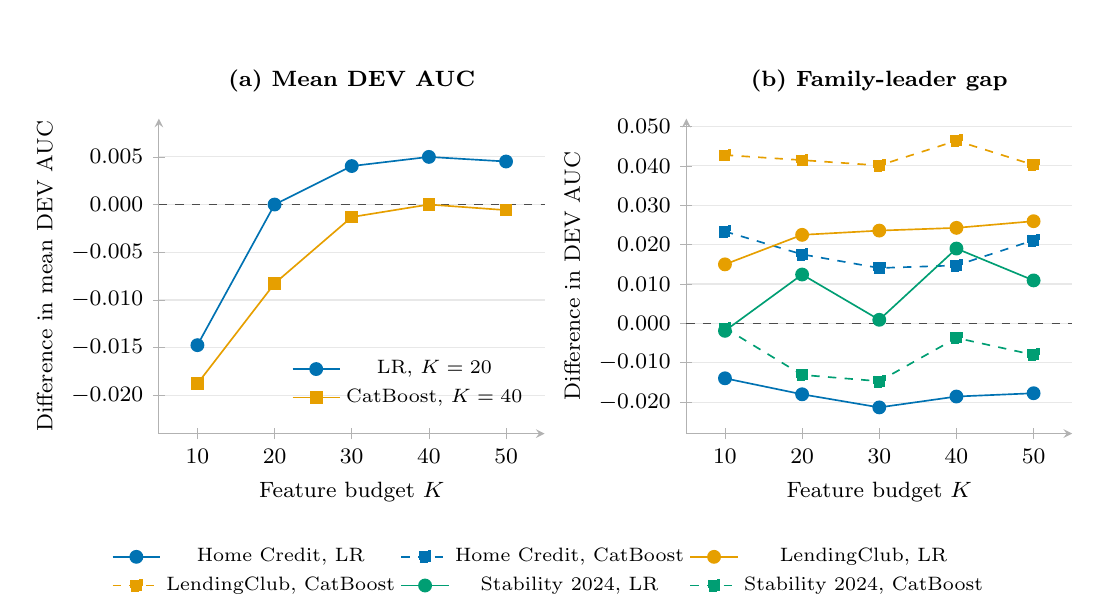
\begin{tikzpicture}
\begin{groupplot}[
    paper,
    group style={group size=2 by 1, horizontal sep=18mm},
    scale only axis, width=4.9cm, height=4.0cm, clip=false,
    xmin=5, xmax=55, xtick={10,20,30,40,50},
    xlabel={Feature budget $\Kfeat$},
    ymajorgrids, axis lines=left,
    yticklabel style={/pgf/number format/fixed, /pgf/number format/precision=3, /pgf/number format/zerofill},
]
\nextgroupplot[title={(a) Mean DEV AUC}, ylabel={Difference in mean DEV AUC}, ymin=-0.024, ymax=0.009, ytick={-0.02,-0.015,-0.01,-0.005,0,0.005},
    legend style={at={(0.98,0.05)}, anchor=south east, draw=none, fill=none, font=\scriptsize}]
\draw[gray!60!black, dashed] (axis cs:5,0) -- (axis cs:55,0);
\addplot[cBlue, semithick, mark=*, mark size=2.2pt] coordinates {(10,-0.014735) (20,0.000000) (30,0.004031) (40,0.004990) (50,0.004506)};
\addlegendentry{LR, $\Kfeat=20$}
\addplot[cOrange, semithick, mark=square*, mark size=2.0pt] coordinates {(10,-0.018775) (20,-0.008273) (30,-0.001311) (40,0.000000) (50,-0.000587)};
\addlegendentry{CatBoost, $\Kfeat=40$}
\nextgroupplot[title={(b) Family-leader gap}, ylabel={Difference in DEV AUC}, ymin=-0.028, ymax=0.052, ytick={-0.02,-0.01,0,0.01,0.02,0.03,0.04,0.05},
    legend to name=budgetlegend, legend columns=3, legend style={draw=none, fill=none, font=\scriptsize}]
\draw[gray!60!black, dashed] (axis cs:5,0) -- (axis cs:55,0);
\addplot[cBlue, semithick, mark=*, mark size=2.2pt] coordinates {(10,-0.013960) (20,-0.018022) (30,-0.021352) (40,-0.018588) (50,-0.017754)};
\addlegendentry{Home Credit, LR}
\addplot[cBlue, semithick, dashed, mark=square*, mark size=2.0pt] coordinates {(10,0.023343) (20,0.017522) (30,0.014054) (40,0.014717) (50,0.021106)};
\addlegendentry{Home Credit, CatBoost}
\addplot[cOrange, semithick, mark=*, mark size=2.2pt] coordinates {(10,0.014980) (20,0.022480) (30,0.023558) (40,0.024256) (50,0.025945)};
\addlegendentry{LendingClub, LR}
\addplot[cOrange, semithick, dashed, mark=square*, mark size=2.0pt] coordinates {(10,0.042744) (20,0.041458) (30,0.040106) (40,0.046391) (50,0.040232)};
\addlegendentry{LendingClub, CatBoost}
\addplot[cGreen, semithick, mark=*, mark size=2.2pt] coordinates {(10,-0.0019) (20,0.0124) (30,0.0009) (40,0.0190) (50,0.0109)};
\addlegendentry{Stability 2024, LR}
\addplot[cGreen, semithick, dashed, mark=square*, mark size=2.0pt] coordinates {(10,-0.0012) (20,-0.0131) (30,-0.0147) (40,-0.0037) (50,-0.0080)};
\addlegendentry{Stability 2024, CatBoost}
\end{groupplot}
\node[anchor=north, yshift=-2mm] at (current bounding box.south) {\pgfplotslegendfromname{budgetlegend}};
\end{tikzpicture}
\caption{Feature-budget sensitivity on development data. (a) Mean development AUC of all selectors of a backbone at each budget, measured against that backbone's documented budget (logistic regression $\Kfeat=20$, CatBoost $\Kfeat=40$; zero by construction at those points). (b) Development AUC of the LLM-assisted family leader minus that of the classical family leader, in each dataset--backbone case; positive values favour LLM-assisted selection. Circles and solid lines are logistic regression, squares and dashed lines CatBoost. No held-out observation enters either panel. Plot code generated with AI assistance from the study's result files (see the declaration on generative AI).}
\label{fig:budgets}
\end{figure*}

\begin{table*}[htbp]
\centering
\footnotesize
\begin{threeparttable}
\caption{Development AUC of the LLM-assisted family leader minus that of the classical family leader, by feature budget; the values plotted in Figure~\ref{fig:budgets}b. Bold marks the documented budget of the backbone. Positive values favour LLM-assisted selection.}
\label{tab:budgets}
\setlength{\tabcolsep}{4pt}
\begin{tabular}{@{}lrrrrr@{}}
\toprule
Case & \multicolumn{5}{c}{Feature budget $\Kfeat$} \\
\cmidrule(l){2-6}
 & 10 & 20 & 30 & 40 & 50 \\
\midrule
Home Credit, LR & $-0.0140$ & $\mathbf{-0.0180}$ & $-0.0214$ & $-0.0186$ & $-0.0178$ \\
Home Credit, CatBoost & $+0.0233$ & $+0.0175$ & $+0.0141$ & $\mathbf{+0.0147}$ & $+0.0211$ \\
LendingClub v2, LR & $+0.0150$ & $\mathbf{+0.0225}$ & $+0.0236$ & $+0.0243$ & $+0.0259$ \\
LendingClub v2, CatBoost & $+0.0427$ & $+0.0415$ & $+0.0401$ & $\mathbf{+0.0464}$ & $+0.0402$ \\
Stability 2024, LR & $-0.0019$ & $\mathbf{+0.0124}$ & $+0.0009$ & $+0.0190$ & $+0.0109$ \\
Stability 2024, CatBoost & $-0.0012$ & $-0.0131$ & $-0.0147$ & $\mathbf{-0.0037}$ & $-0.0080$ \\
\bottomrule
\end{tabular}
\end{threeparttable}
\end{table*}


\section{Headline subsets}
\label{app:subsets}
\setcounter{table}{0}\setcounter{figure}{0}

This appendix's lists, the twelve subsets behind Table~\ref{tab:primary_results}, are the features selected by the frozen full-DEV refit of the LLM-assisted family leader and of the classical family leader in each dataset--backbone case, in the order the selector produced them ($\Kfeat=20$ for logistic regression, $\Kfeat=40$ for CatBoost). They are given in full in the supplementary material, Tables~S1 to S6, two tables per dataset (ranks 1 to 20 of all four subsets, then ranks 21 to 40 of the two CatBoost subsets), and as \texttt{headline\_subsets.csv} in the repository. For pure LLM the order is that of the cached full-DEV ranking; on Stability 2024 one ranking served both backbones, so its logistic-regression subset is the first twenty names of its CatBoost subset. Feature names are those of the engineered universes of Section~\ref{subsec:datasets}; on Home Credit the three external scores occupy the first three ranks of the pure LLM list, as noted in Section~\ref{subsec:obfuscation_results}. The two leaders' subsets overlap little: they share 4 of 20 (logistic regression) and 16 of 40 (CatBoost) features on Home Credit, 4 of 20 and 21 of 40 on LendingClub v2, and 1 of 20 and 4 of 40 on Stability 2024.

\section{Development of the protocol}
\label{app:protocol}
\setcounter{table}{0}\setcounter{figure}{0}

% author-confirmed: every protocol version was developed and compared on the five development folds; no held-out population was scored before the final pipelines were frozen; the values quoted for the superseded versions in Table E.1 are development-fold means.
The protocol of Section~\ref{sec:methodology} is the final form of an evaluation developed through successive versions on development data, and the final results supersede the earlier ones. Table~\ref{tab:stages} records the changes that mattered and their development-fold outcomes. Every version was developed and compared on the five development folds of Section~\ref{subsec:dev_oot}; no held-out population was scored before the final pipelines were frozen, and each frozen pipeline then scored its held-out population once; the controls added at revision were each scored once afterwards (last row of Table~\ref{tab:stages}). The DEV/HO design of Home Credit and LendingClub was fixed from the outset, and the Stability 2024 cutoff, 2020-02-26, was fixed when that dataset was added (Section~\ref{subsec:dev_oot}). What changed across versions was the comparator set, the semantic inputs of the LLM stage, the statistical selector used as the classical reference, and the inference procedure.

% author-confirmed: the contrastive-representation selector was dropped before any of its held-out results existed, as out of scope; on the development folds it lay below both family leaders in every case.
One method was dropped from the strategy set between the three-dataset version and the final evaluation: a contrastive-representation selector, together with the Home Credit voting family built on it (\ref{app:voting}). The selector encodes each candidate record with MiniLM sentence embeddings \cite{wang2020minilm,reimers2019}, aligns them by a CLIP-style contrastive objective \cite{radford2021} with label-free distribution descriptors of each feature computed on DEV training rows, and ranks the features by similarity to an anchor set of temporally stable features; it reads rows but no outcomes. It is neither a classical selector nor the LLM pre-screener under study, so it belonged to neither family of the comparison. It was dropped before the held-out run, when no held-out result of it existed, and on the development folds it lay below both family leaders in every case, so its removal changed no leader and no comparison; its held-out stage never ran before this revision. The thirteen strategies of Table~\ref{tab:methods} and the full-feature reference were then frozen. At revision the selector returns as a control outside both families, alone, with its pool refined by the second stage of LLM then mRMR, and fused with the semantic ranking (Section~\ref{subsec:classical_fs}), with the results of Sections~\ref{subsec:robustness} and \ref{subsec:stability_results}.

Three design decisions were made on development evidence. First, the comparator changed from a single mRMR baseline on two datasets to the classical selector of highest AUC in each case, drawn from the full selector set on three datasets; the LLM-assisted comparator is chosen in the same way. Applied to the held-out results, this choice of both headline methods is why the HO-rule comparisons of Table~\ref{tab:primary_results} are descriptive (Section~\ref{subsec:inference}). The development-data rule of Table~\ref{tab:confirmatory}, which chooses each family's leader on the mean DEV fold AUC and is the only development-data rule specified, and the mixed rule of Section~\ref{subsec:primary_results} were added when the paper was revised; they re-pair selectors already scored in the single held-out run, with no refitting or rescoring, and use no held-out information in the choice. Second, the way feature descriptions are prepared for the language model was revised. In the early versions semantic explanations were written after feature selection; in the revised process the descriptions are prepared before LLM ranking, starting from the source-variable definition and stating the aggregation operation and time window in words, so that, for example, the mean of a bureau annuity amount over the records of a case is described as the average bureau annuity amount of the case. The revision was intended to give the language model accurate meanings for the engineered features. The three provenances of the descriptions and the template clause for engineered features are described in Section~\ref{subsec:llm_fs}. No held-out result existed when the descriptions took their present form, and because the base definitions are documentation entries and every engineered clause is generated by the same template, there was no per-feature step at which any result could have influenced the phrasing. Whether the results depend on that phrasing was tested directly: with every description rebuilt from lineage alone, held-out AUC moves by no more than 0.0074 in the eight re-run pipelines, inside the materiality bar in each (Section~\ref{subsec:mechanical_results}). Third, the mutual-information mRMR of the final protocol replaced the RF/correlation filter of the early versions as the stand-alone statistical selector; the RF/correlation implementation remains the reference of the voting family (\ref{app:voting}), which is why its Home Credit logistic-regression reference (0.7448) differs from the mutual-information mRMR value of Table~\ref{tab:primary_results} (0.7699), and the second stage of LLM then mRMR on Home Credit and LendingClub, whose pipelines were frozen with it (Section~\ref{subsec:hybrid_fs}); on Stability 2024, added later, that second stage is the mutual-information implementation.

Three inference changes altered what could be claimed rather than the estimates. Five-fold rank tests on the development folds, whose minimum attainable two-sided $p$-value with five non-zero pairs is 0.0625, gave way to paired inference on matched HO observations; the six headline comparisons are reported with paired bootstrap confidence intervals and without observation-level significance claims, because under the HO rule the identities of the compared methods are determined from the HO results, and the Holm-adjusted DeLong tests that an intermediate revision attached to the development-rule comparison were withdrawn for the reason given in Section~\ref{subsec:inference}. The third change, in the revision reported here, tests the comparison at the level of the case instead: an exact Wilcoxon signed-rank test over the six paired differences of each rule, computed from the reported differences without refitting or rescoring. The DeLong test with Holm adjustment was extended at the same revision to the LLM-vote arm of the voting family, fixed in a protocol file before its held-out scoring; the semantic controls carry bootstrap intervals only (Section~\ref{subsec:inference}).

\begin{table*}[htbp]
\centering
\footnotesize
\setlength{\tabcolsep}{5pt}
\begin{threeparttable}
\caption{Protocol versions and the final evaluation. The versions above the last two rows were developed and compared on the five development folds, and no held-out population was scored in any of them; the values quoted for them are mean development-fold AUCs computed with earlier comparator sets, earlier semantic inputs and, in the earliest versions, the RF/correlation filter as the mRMR reference. The last three rows are the evaluation reported in this paper: the single held-out scoring run and its revision.}
\label{tab:stages}
\begin{tabular}{@{}L{27mm}L{\dimexpr(\textwidth-27mm-4\tabcolsep)/2\relax}L{\dimexpr(\textwidth-27mm-4\tabcolsep)/2\relax}@{}}
\toprule
Protocol version & Change to the methodology & Development-fold outcome, and why (superseded values) \\
\midrule
Home Credit comparison & 16 pipelines on the 373 screened features; the LLM produces a top-100 pool refined by mRMR, Boruta or a stable-core rule; six LLM calls reused across pipelines. & Best mean development-fold AUC from CatBoost with LLM then mRMR (0.772 against 0.769 for mRMR). A variant whose LLM shortlist was almost as small as the budget gave no gain, so the LLM was fixed as a broad first-pass screener rather than the final selector. \\
\addlinespace
Two-dataset canonical comparison & Home Credit and LendingClub, four selectors, 16 runs; five-fold exact Wilcoxon tests; type-aware feature PSI repaired for 480 selected-feature occurrences; usage and cost accounting. & No fold test could reach $p<0.05$ (minimum attainable 0.0625), so fold tests were abandoned as underpowered; direct API cost bounded at USD 0.171 to 0.413. \\
\addlinespace
Matched-observation inference and voting & Paired DeLong tests and 2,000-resample paired bootstrap on matched observation identifiers, Holm correction within families, specified for the final held-out run; eight voting variants added. & On the development validation partitions, 11 of 12 canonical differences were significant, with dataset-dependent signs; voting exceeded sequential screening in 5 of 8 variants and full-pool mRMR in none. \\
\addlinespace
Three-dataset evaluation & Stability 2024 added (HO cutoff 2020-02-26); fourteen selectors and a full-feature reference; revised semantic representation of the features supplied to the LLM; per-case classical family leader as comparator. & On the development folds the LLM-assisted leader led five of six cases at the point-estimate level; the family-leader comparator lowered the apparent LLM advantage relative to the two-dataset comparison. \\
\addlinespace
Cross-dataset classical voting & Pre-declared family of twelve comparisons on Home Credit and LendingClub: three classical voters (RF/correlation mRMR, Boruta, RFE), pools of 100, 200 and 300, RF/correlation mRMR reference on the candidate set. & Family fixed in a protocol file in this version; its twelve held-out comparisons were computed in the final run below, all positive and Holm-significant, from $+0.0020$ to $+0.0129$ AUC (\ref{subsec:voting_results}). \\
\addlinespace
Final evaluation (single held-out scoring run) & The contrastive-representation selector of the three-dataset version and the Home Credit voting family built on it dropped from the strategy set as out of scope before the held-out run (see text; both return as controls at revision), leaving the thirteen strategies of Table~\ref{tab:methods}; pipelines frozen and each held-out population scored once by them; six paired comparisons between HO-chosen family leaders with bootstrap confidence intervals, reported descriptively, and six development-rule comparisons between DEV-chosen leaders, at that stage with Holm-adjusted paired DeLong tests; exact AUC precision; mutual-information mRMR distinguished from the RF/correlation filter, which remains the second stage of LLM then mRMR on Home Credit and LendingClub. & Results of Section~\ref{sec:results}. \\
\addlinespace
Revision reported in this paper (reporting) & Reporting changes with no headline pipeline refitted or rescored: the Holm-adjusted DeLong tests of the development-rule comparison withdrawn in favour of effect sizes with paired bootstrap intervals, the test retained only for the pre-declared classical voting family; a third leader rule (development-chosen LLM-assisted leader against held-out-best classical leader) and the development-to-holdout change of each leader added; an exact Wilcoxon signed-rank test over the six paired differences of each rule added. & No headline AUC, interval, subset or stability value moves; across the six cases the signed-rank test gives two-sided $p=0.063$ under the DEV rule (one-sided $0.031$) and $0.219$ under the HO and mixed rules; the five-of-six result holds under the third rule with the margins of Table~\ref{tab:primary_results}; the classical leaders lose more AUC from development to holdout than the LLM-assisted leaders, so the two original rules are not independent checks (Section~\ref{subsec:primary_results}). \\
\addlinespace
Revision reported in this paper (voting arm and semantic controls) & New pipelines outside both families, each fixed in a protocol file with the rule for reading it after the headline results were known and before its own single held-out scoring: the semantic ranking as a fourth equal-weight voter in the rank-voting design on all three datasets, with the classical vote also run on Stability 2024 (the Stability 2024 extension and its six-case rule fixed after the Home Credit and LendingClub results of the arm were known); a text-embedding ranking (BGE-large, one query), alone and with the second stage of LLM then mRMR; the contrastive ranking of the three-dataset version with that second stage; and the equal-weight fusion of the semantic and contrastive rankings, the contrastive ranking refitted in each fold on that fold's training rows. No new call to the language model; the frozen rankings, predictions, folds, budgets, backbone configurations and seeds reused; the published classical-vote, pure LLM and LLM-then-mRMR held-out values and the held-out row counts reproduced from the frozen artefacts before any new value was computed. & No headline AUC, interval, subset or stability value moves. The LLM vote exceeds the classical vote in all eighteen configurations and clears the bar at the primary pool in four of six cases (\ref{subsec:voting_results}); the text-embedding and contrastive controls lie below their LLM counterparts in every case, beyond the bar in five of six, and below every classical leader (Section~\ref{subsec:robustness}); the fusion is less reproducible than the stable-core construction and below pure LLM in held-out AUC in all six cases, beyond the bar in four (Section~\ref{subsec:stability_results}). \\
\bottomrule
\end{tabular}
\end{threeparttable}
\end{table*}

\section{Robustness checks in detail}
\label{app:robustness}
\setcounter{table}{0}\setcounter{figure}{0}

This appendix gives the detail behind the robustness checks summarised in Table~\ref{tab:robustness} (Section~\ref{subsec:robustness}), with Tables~\ref{tab:lc_maturity}, \ref{tab:diversity} and \ref{tab:dimension}, and the unmatched wall-clock times referred to in Section~\ref{subsec:cost_runtime}.

\paragraph{L1-penalised selector}
An L1-penalised logistic regression selector, run afterwards on the same candidate sets, folds and budgets (\texttt{liblinear}, $C=0.05$ fixed and untuned, balanced class weights, standardised median-imputed inputs with ordinal-coded categoricals, the $\Kfeat$ largest non-zero coefficients retained without padding, and the subsets refitted with the fixed backbones of Section~\ref{subsec:models}), attains held-out AUC of 0.674 to 0.842 and lies below the classical family leader in every case, by 0.005 on LendingClub CatBoost and 0.009 on Stability 2024 CatBoost and by 0.026 to 0.096 elsewhere, so its inclusion would change no leader and no comparison.

\paragraph{Semantic controls}
The four semantic controls of Section~\ref{subsec:classical_fs}, run at revision on the same candidate sets, folds and budgets with no new call to the language model and each scored once on the holdout under a rule fixed beforehand, are reported in Table~\ref{tab:semantic_controls} against the LLM-assisted pipeline each modifies or replaces, on identical held-out observations with the paired bootstrap of Section~\ref{subsec:inference}. The text-embedding ranking attains held-out AUC of 0.6796 to 0.8153 and lies below pure LLM in every case, by $0.0352$ to $0.0606$ with intervals excluding zero in five cases and by $0.0062$ on Home Credit logistic regression; with the second stage of LLM then mRMR applied to its top 60 or 100 names it lies below LLM then mRMR by $0.0331$ to $0.0915$ in the same five cases and by $0.0091$ on Home Credit logistic regression. The contrastive ranking with that second stage lies below LLM then mRMR by $0.0252$ to $0.0912$ in five cases and by $0.0079$ on Home Credit logistic regression. All three lie below the classical leader of their case, by $0.0231$ to $0.0649$, so their inclusion would change no leader and no comparison. The fusion of the semantic and contrastive rankings lies below pure LLM in all six cases, by $0.0015$ to $0.0258$, beyond the bar in four; its fold-to-fold reproducibility is reported in Table~\ref{tab:stability}. The text-embedding ranking is one list per dataset, so its five fold subsets coincide and its stability is 1 by construction; the stability of the other controls comes from five fold refits over the candidate set of the dataset.

\begin{table*}[htbp]
\centering
\scriptsize
\setlength{\tabcolsep}{2pt}
\begin{threeparttable}
\caption{Semantic controls (Section~\ref{subsec:classical_fs}) against their LLM-assisted counterparts on paired HO observations. $\Delta$ is the counterpart minus the control, with its 95\% paired percentile bootstrap interval (2,000 resamples, seed 20260721); Nogueira stability is computed over the five fold subsets with $d$ = the candidate set (373, 675 and 1,068), Jaccard is the mean pairwise fold Jaccard, and Shared is the number of features common to the control's and the counterpart's full-DEV subsets (not recorded for the fusion). The counterpart of the text-embedding ranking and of the fusion is pure LLM; that of the two filtered controls is LLM then mRMR. The text-embedding ranking is one list per dataset, so its fold agreement is 1 by construction.}
\label{tab:semantic_controls}
\begin{tabular}{@{}llrlrlrrr@{}}
\toprule
Case & Control & AUC & Counterpart (AUC) & $\Delta$AUC & 95\% CI & Nogueira & Jaccard & Shared \\
\midrule
Home Credit, LR & Text-embedding ranking & 0.7374 & Pure LLM (0.7436) & $+0.0062$ & $[0.0048,\,0.0082]$ & 1.0000 & 1.0000 & 11 \\
 & Text-embedding then filter & 0.7341 & LLM then mRMR (0.7432) & $+0.0091$ & $[0.0068,\,0.0109]$ & 0.6417 & 0.5013 & 9 \\
 & Contrastive ranking then filter & 0.7353 & LLM then mRMR (0.7432) & $+0.0079$ & $[0.0067,\,0.0095]$ & 0.7832 & 0.6682 & 12 \\
 & LLM + contrastive fusion & 0.7421 & Pure LLM (0.7436) & $+0.0015$ & $[0.0002,\,0.0029]$ & 0.6249 & 0.4833 & -- \\
\addlinespace
Home Credit, CatBoost & Text-embedding ranking & 0.7583 & Pure LLM (0.7935) & $+0.0352$ & $[0.0326,\,0.0370]$ & 1.0000 & 1.0000 & 33 \\
 & Text-embedding then filter & 0.7427 & LLM then mRMR (0.7758) & $+0.0331$ & $[0.0314,\,0.0351]$ & 0.6935 & 0.5769 & 31 \\
 & Contrastive ranking then filter & 0.7506 & LLM then mRMR (0.7758) & $+0.0252$ & $[0.0223,\,0.0275]$ & 0.5718 & 0.4552 & 34 \\
 & LLM + contrastive fusion & 0.7812 & Pure LLM (0.7935) & $+0.0123$ & $[0.0101,\,0.0147]$ & 0.5548 & 0.4353 & -- \\
\addlinespace
LendingClub v2, LR & Text-embedding ranking & 0.6796 & Pure LLM (0.7402) & $+0.0606$ & $[0.0596,\,0.0623]$ & 1.0000 & 1.0000 & 10 \\
 & Text-embedding then filter & 0.6741 & LLM then mRMR (0.7179) & $+0.0438$ & $[0.0425,\,0.0447]$ & 0.7264 & 0.5871 & 12 \\
 & Contrastive ranking then filter & 0.6718 & LLM then mRMR (0.7179) & $+0.0461$ & $[0.0448,\,0.0479]$ & 0.5893 & 0.4389 & 9 \\
 & LLM + contrastive fusion & 0.7186 & Pure LLM (0.7402) & $+0.0216$ & $[0.0202,\,0.0231]$ & 0.6393 & 0.4892 & -- \\
\addlinespace
LendingClub v2, CatBoost & Text-embedding ranking & 0.6818 & Pure LLM (0.7335) & $+0.0517$ & $[0.0508,\,0.0523]$ & 1.0000 & 1.0000 & 21 \\
 & Text-embedding then filter & 0.6792 & LLM then mRMR (0.7707) & $+0.0915$ & $[0.0909,\,0.0926]$ & 0.6581 & 0.5207 & 19 \\
 & Contrastive ranking then filter & 0.6795 & LLM then mRMR (0.7707) & $+0.0912$ & $[0.0904,\,0.0917]$ & 0.8046 & 0.6894 & 23 \\
 & LLM + contrastive fusion & 0.7263 & Pure LLM (0.7335) & $+0.0072$ & $[0.0065,\,0.0080]$ & 0.6678 & 0.5282 & -- \\
\addlinespace
Stability 2024, LR & Text-embedding ranking & 0.7717 & Pure LLM (0.8322) & $+0.0605$ & $[0.0589,\,0.0627]$ & 1.0000 & 1.0000 & 11 \\
 & Text-embedding then filter & 0.7532 & LLM then mRMR (0.8112) & $+0.0580$ & $[0.0554,\,0.0599]$ & 0.7049 & 0.5586 & 10 \\
 & Contrastive ranking then filter & 0.7629 & LLM then mRMR (0.8112) & $+0.0483$ & $[0.0470,\,0.0500]$ & 0.5862 & 0.4297 & 13 \\
 & LLM + contrastive fusion & 0.8094 & Pure LLM (0.8322) & $+0.0228$ & $[0.0208,\,0.0247]$ & 0.6994 & 0.5573 & -- \\
\addlinespace
Stability 2024, CatBoost & Text-embedding ranking & 0.8153 & Pure LLM (0.8716) & $+0.0563$ & $[0.0537,\,0.0584]$ & 1.0000 & 1.0000 & 32 \\
 & Text-embedding then filter & 0.8008 & LLM then mRMR (0.8519) & $+0.0511$ & $[0.0497,\,0.0533]$ & 0.6738 & 0.5302 & 34 \\
 & Contrastive ranking then filter & 0.8082 & LLM then mRMR (0.8519) & $+0.0437$ & $[0.0409,\,0.0462]$ & 0.7901 & 0.6848 & 31 \\
 & LLM + contrastive fusion & 0.8458 & Pure LLM (0.8716) & $+0.0258$ & $[0.0237,\,0.0281]$ & 0.6468 & 0.5018 & -- \\
\bottomrule
\end{tabular}
\end{threeparttable}
\end{table*}

\paragraph{Native categorical handling}
The one-hot encoding of Section~\ref{subsec:preprocessing} is likewise not what carries the ordering. Re-running the three CatBoost cases with CatBoost's native categorical handling in place of one-hot expansion, the same forty features, configuration and seed, moves every held-out AUC by at most $0.005$ and leaves the family ordering unchanged in all three: pure LLM 0.7918 against RFE CatBoost 0.7816 on Home Credit, LLM then mRMR 0.7738 against IV then Boruta 0.7203 on LendingClub v2, and pure LLM 0.8716 against CatBoost SHAP 0.8532 on Stability 2024, margins of $+0.010$, $+0.054$ and $+0.018$ against $+0.012$, $+0.051$ and $+0.021$ under one-hot. The Stability 2024 pure LLM subset contains no categorical features, so its value is unchanged by construction.

\paragraph{LendingClub resolved-loan population: matured cohort, term and issue month}
The largest difference, $+0.051$ on LendingClub with CatBoost, sits on the population with the strongest known selection artefact: only loans resolved by the 2019-05-01 snapshot are evaluated, a restriction that over-represents early defaults and early repayments and raises the HO event rate from 19.5\% in DEV to 23.3\% (Section~\ref{subsec:dev_oot}). The restriction applies to the evaluation population and not to any selector: all thirteen selectors are scored on the same 293,105 loans, so it shifts the level of every AUC in this column rather than acting differentially on one family. Whether the retained population favours the kind of signal one family selects, early default rather than late, is tested directly in the next paragraph.

That test re-scores the LendingClub comparison of Table~\ref{tab:primary_results} on the frozen HO prediction vectors as row filters, with no refitting, and bootstraps each filtered set by the routine of Section~\ref{subsec:inference}. The pre-declared filter is the cohort that could have matured before the snapshot: the 123,898 36-month loans issued 2016-01 to 2016-05, every one of which had reached its term by 2019-05-01, so the resolution filter cannot act on it. The comparison is also resolved by term and by issue month. Table~\ref{tab:lc_maturity} reports the matured cohort and the two terms. The LLM-assisted leader has the higher AUC in all thirty comparisons, every interval excludes zero, and the difference clears the materiality bar of $0.010$ on the matured cohort and within each term under both backbones: $+0.018$ and $+0.011$ on the matured cohort, $+0.022$ and $+0.012$ on the 36-month loans and $+0.014$ and $+0.010$ on the 60-month loans. Resolved by issue month, the difference is positive in all twelve months of 2016 under both backbones. The margins are smaller on these sub-populations than on the pooled holdout, where the loans of different terms and vintages are ranked together; the direction of the comparison and its materiality do not depend on the resolution filter.

\paragraph{Source concentration: family cap and depth-0 controls}
A subset drawn from few source tables invites the objection that any rule concentrating on the same tables would do as well: the pure LLM subsets on Stability 2024 are drawn entirely from \texttt{static\_0} under both budgets, and on Home Credit CatBoost 26 of the 40 features are bureau aggregates, whereas the classical leaders of those cases spread across six or seven source families (\ref{app:subsets}). The two diversity controls of Section~\ref{subsec:classical_fs} test it, and Table~\ref{tab:diversity} reports them. Capping the classical leader per source family lowers it in all six cases, by $0.009$ to $0.069$, so the cap binds; the capped selector remains below the LLM-assisted leader of its case by $0.021$ to $0.083$ in five of the six. On Home Credit logistic regression, the one case the classical selector wins, the cap erases that lead: mRMR falls from $0.7699$ to $0.7457$ against the LLM-assisted leader's $0.7489$, leaving the two families level within the bar. On Stability 2024 the sharper test is the depth-0 restriction, which confines the classical leader to the two static tables the semantic ranking chose from: it reaches $0.7804$ with logistic regression and $0.8231$ with CatBoost, against $0.8322$ and $0.8716$ for pure LLM over the same pool, a shortfall of $0.052$ and $0.049$. Source concentration alone therefore does not reproduce the Stability 2024 margins, and the semantic reading of those two cases stands with the control reported as the test it passed.

\paragraph{Stability 2024 monthly breakdown}
The Stability 2024 comparison was also resolved by month of decision over the nine calendar months that its held-out window, 26 February to 5 October 2020, touches; the window holds the last four days of February and the first five days of October, so those two months are partial. The monthly decision counts are 10,952 (26--29 February), 60,748 (March), 8,289 (April), 28,725 (May), 45,962 (June), 28,912 (July), 50,831 (August), 61,905 (September) and 8,592 (1--5 October). Pure LLM has the higher AUC in every one of the nine months under both backbones, by $+0.010$ to $+0.020$ against RFE CatBoost with logistic regression and by $+0.012$ to $+0.029$ against CatBoost SHAP with CatBoost, above the materiality bar in every month, so the direction of the comparison does not depend on the period within the window. The window contains a sharp break in volume that coincides with the onset of the COVID-19 pandemic (Section~\ref{subsec:cross_dataset}).

\paragraph{Boruta budget attainment}
The low held-out AUC of LLM then Boruta (Section~\ref{subsec:primary_results}) is not an artefact of short subsets: over the 108 fold and full-DEV refits of the three Boruta-based selectors (Boruta RF, IV then Boruta and LLM then Boruta; six cases, six partitions each) the Boruta stage reached its budget in 104, every full-DEV refit among them, and LLM then Boruta fell short only once, on Stability 2024 CatBoost fold 1 with 35 of 40 features; the other three below-budget cells are Boruta RF on Home Credit CatBoost fold 1 (26 of 40) and IV then Boruta on Home Credit CatBoost folds 1 and 2 (20 and 39 of 40).

\paragraph{Effective dimension of the headline subsets}
The budget counts original variables, not columns (Section~\ref{subsec:preprocessing}), so a subset that contains categorical variables delivers more than $\Kfeat$ columns to its model. Table~\ref{tab:dimension} gives $\Kfeat$ and the column count for the twelve headline subsets, after the full-DEV preprocessing map of each backbone. The widest input anywhere in the study is 174 columns, the CatBoost SHAP subset of Stability 2024 at $\Kfeat=40$, whose nine categorical variables carry the expansion; the LLM-assisted leader of that case receives 40. The LLM-assisted leader receives fewer columns than the classical leader in five of the six cases, by 5 to 134 columns, so in those five the margin is not obtained on a wider input matrix. Home Credit with CatBoost is the exception: the pure LLM subset carries five categorical variables, which expand to 37 of its 72 columns, against three in the RFE CatBoost wrapper, which expand to 13 of its 50. Its $+0.012$, the smallest of the five positive differences, is therefore obtained on the wider matrix of the two, and should be read with the native-categorical re-run reported above, where no expansion takes place and the same comparison stands at $+0.010$. One subset is budgeted on the expanded scale rather than the original one, the LLM then mRMR leader of LendingClub v2 with CatBoost (Section~\ref{subsec:preprocessing}): 13 of its 40 slots are one-hot indicators drawn from seven original variables, so it spans 34 original variables in 40 columns, against 40 original variables in 77 columns for its classical comparator, fewer on both scales. These counts change no leader, no difference and no interval; they are reported because $\Kfeat$ and the input width are not the same quantity and only the first is fixed by the design.

\paragraph{Unmatched wall-clock times}
Wall-clock times were not measured under matched conditions, with the one exception reported in Section~\ref{subsec:cost_runtime}, an mRMR pass over the unscreened 1,959-feature universe of Stability 2024 against one over a 100-feature pool, and support no scalability claim. On Home Credit logistic regression the pure LLM pipeline took 0.8 minutes against 12.1 minutes for full-pool mRMR (RF/correlation implementation) and 24.6 minutes for stable core plus LLM fill. On LendingClub CatBoost pure LLM was slower than mRMR: domain rules took 49.7 minutes, mRMR 65.3, LLM then mRMR 72.8, pure LLM 73.8, PCA 88.0, LLM then Boruta 110.5, Boruta 172.6 and stable core plus LLM fill 256.0 minutes, of which 176.6 minutes were feature selection; measured against the 49.7 minutes of the essentially selection-free domain-rules pipeline, it is the selection stage rather than model fitting that separates the pipelines, and the semantic call is negligible beside both. Runtimes were measured under unequal caching and execution conditions and are quoted here for Home Credit and LendingClub only.

\begin{table}[htbp]
\centering
\footnotesize
\begin{threeparttable}
\caption{LendingClub v2 held-out comparison of Table~\ref{tab:primary_results} re-scored on sub-populations of the holdout, as row filters on the frozen HO prediction vectors with no refitting. The matured cohort is the 36-month loans issued 2016-01 to 2016-05, all of which had reached term before the 2019-05-01 snapshot, so the resolution filter of Section~\ref{subsec:dev_oot} cannot act on it; the two terms partition the holdout. $\Delta$AUC is the LLM-assisted leader minus the classical leader (bar: Section~\ref{subsec:inference}).}
\label{tab:lc_maturity}
\setlength{\tabcolsep}{5pt}
\begin{tabular}{@{}lrrr@{}}
\toprule
Sub-population & $n$ & LR & CatBoost \\
\midrule
Matured cohort\tnote{a} & 123,898 & $+0.0183$ & $+0.0112$ \\
Term 36 months & 232,361 & $+0.0215$ & $+0.0122$ \\
Term 60 months & 60,744 & $+0.0141$ & $+0.0101$ \\
\bottomrule
\end{tabular}
\begin{tablenotes}\footnotesize
\item[a] Paired 95\% bootstrap intervals on the matured cohort: $[+0.0159,\,+0.0207]$ with logistic regression and $[+0.0099,\,+0.0126]$ with CatBoost. Every interval of every sub-population reported here and by issue month excludes zero; the full set, with the AUC of each leader, is in the repository.
\end{tablenotes}
\end{threeparttable}
\end{table}

\begin{table*}[htbp]
\centering
\footnotesize
\begin{threeparttable}
\caption{Diversity controls on the headline comparison (Section~\ref{subsec:robustness}). \emph{Family cap} re-runs the HO-rule classical leader of each case with at most $\lceil \Kfeat/F\rceil$ features per source family; \emph{depth-0} restricts it to the depth-0 candidates of Stability 2024. Both are fitted on full DEV with the frozen backbones and scored once on HO. ``Uncapped'' is the classical leader's own HO AUC (Table~\ref{tab:primary_results}) and ``LLM-assisted'' its LLM-assisted counterpart in the same case; the last column is the control minus that counterpart (bar: Section~\ref{subsec:inference}). The controls are not selectors of the comparison and appear in no family, leader or count.}
\label{tab:diversity}
\setlength{\tabcolsep}{5pt}
\begin{tabular}{@{}llllrrrr@{}}
\toprule
Case & Rule & Base selector & $\Kfeat$ & Control & Uncapped & LLM-assisted & Difference \\
\midrule
Home Credit, LR & Family cap & mRMR & 20 & 0.7457 & 0.7699 & 0.7489 & $-0.003$\tnote{a} \\
Home Credit, CatBoost & Family cap & RFE CatBoost & 40 & 0.7721 & 0.7814 & 0.7935 & $-0.021$ \\
LendingClub v2, LR & Family cap & IV then Boruta & 20 & 0.6849 & 0.7098 & 0.7402 & $-0.055$ \\
LendingClub v2, CatBoost & Family cap & IV then Boruta & 40 & 0.7065 & 0.7201 & 0.7707 & $-0.064$ \\
Stability 2024, LR & Family cap & RFE CatBoost & 20 & 0.7494 & 0.8181 & 0.8322 & $-0.083$ \\
Stability 2024, CatBoost & Family cap & CatBoost SHAP & 40 & 0.8289 & 0.8509 & 0.8716 & $-0.043$ \\
\addlinespace
Stability 2024, LR & Depth-0 & RFE CatBoost & 20 & 0.7804 & 0.8181 & 0.8322 & $-0.052$ \\
Stability 2024, CatBoost & Depth-0 & CatBoost SHAP & 40 & 0.8231 & 0.8509 & 0.8716 & $-0.049$ \\
\bottomrule
\end{tabular}
\begin{tablenotes}\footnotesize
\item[a] The classical selector wins this case uncapped (0.7699); the cap removes that lead and leaves the two families level within the materiality bar.
\end{tablenotes}
\end{threeparttable}
\end{table*}

\begin{table}[htbp]
\centering
\scriptsize
\begin{threeparttable}
\caption{Effective dimension of the twelve headline subsets of Table~\ref{tab:primary_results}. ``Cat.'' is the number of the $\Kfeat$ selected original variables that are categorical; ``Columns'' is the number of columns the backbone receives after the full-DEV preprocessing map of Section~\ref{subsec:preprocessing}, with an explicit missing token per categorical and levels below the minimum frequency dropped (10 observations for Home Credit and Stability 2024, 50 for LendingClub v2). Subsets with no categorical variable receive exactly $\Kfeat$ columns.}
\label{tab:dimension}
\setlength{\tabcolsep}{4pt}
\begin{tabular}{@{}lrrr@{}}
\toprule
Selector & $\Kfeat$ & Cat. & Columns \\
\midrule
\multicolumn{4}{@{}l}{\emph{Home Credit, LR}} \\
Stable core + LLM fill & 20 & 0 & 20 \\
mRMR & 20 & 3 & 33 \\
\addlinespace
\multicolumn{4}{@{}l}{\emph{Home Credit, CatBoost}} \\
Pure LLM & 40 & 5 & 72 \\
RFE CatBoost & 40 & 3 & 50 \\
\addlinespace
\multicolumn{4}{@{}l}{\emph{LendingClub v2, LR}} \\
Pure LLM & 20 & 5 & 43 \\
IV then Boruta & 20 & 5 & 48 \\
\addlinespace
\multicolumn{4}{@{}l}{\emph{LendingClub v2, CatBoost}} \\
LLM then mRMR\tnote{a} & 40 & 0 & 40 \\
IV then Boruta & 40 & 7 & 77 \\
\addlinespace
\multicolumn{4}{@{}l}{\emph{Stability 2024, LR}} \\
Pure LLM & 20 & 0 & 20 \\
RFE CatBoost & 20 & 1 & 28 \\
\addlinespace
\multicolumn{4}{@{}l}{\emph{Stability 2024, CatBoost}} \\
Pure LLM & 40 & 0 & 40 \\
CatBoost SHAP & 40 & 9 & 174 \\
\bottomrule
\end{tabular}
\begin{tablenotes}\footnotesize
\item[a] The only headline subset budgeted on the expanded scale (Section~\ref{subsec:preprocessing}): 13 of its 40 slots are one-hot indicators of seven original variables, so it spans 34 original variables. The LLM-assisted leader of each case is listed first.
\end{tablenotes}
\end{threeparttable}
\end{table}

\begin{table*}[htbp]
\centering
\footnotesize
\begin{threeparttable}
\caption{Agreement among the cached semantic responses of Table~\ref{tab:response_spread}: Nogueira stability and mean pairwise Jaccard of the draws over the screened candidate set ($d$ = 373, 675 and 1,068; the Home Credit and LendingClub rows are the pure LLM rows of Table~\ref{tab:stability}), the number of the $\Kfeat$ names present in every draw, and the number of distinct names the draws span together.}
\label{tab:response_lists}
\setlength{\tabcolsep}{5pt}
\begin{tabular}{@{}llrrrrrr@{}}
\toprule
Case & Model & $\Kfeat$ & Draws & Nogueira & Jaccard & Names in all draws & Distinct names \\
\midrule
Home Credit & LR & 20 & 5 & 0.5403 & 0.4076 & 6 & 42 \\
Home Credit & CatBoost & 40 & 5 & 0.4092 & 0.3149 & 8 & 98 \\
LendingClub v2 & LR & 20 & 5 & 0.5517 & 0.4011 & 4 & 39 \\
LendingClub v2 & CatBoost & 40 & 5 & 0.6280 & 0.4828 & 14 & 71 \\
\addlinespace
Stability 2024 & LR & 20 & 10 & 0.8052 & 0.6908 & 11 & 30 \\
Stability 2024 & CatBoost & 40 & 10 & 0.7766 & 0.6506 & 22 & 69 \\
\bottomrule
\end{tabular}
\end{threeparttable}
\end{table*}

\begin{table*}[htbp]
\centering
\footnotesize
\setlength{\tabcolsep}{5pt}
\begin{threeparttable}
\caption{Cost structure of the pipeline stages, as it follows from the method definitions of Sections~\ref{subsec:classical_fs}, \ref{subsec:llm_fs} and \ref{subsec:hybrid_fs}; a description of the design, not a measurement. ``Recomputed'' states how often the stage runs in the protocol; ``Cost grows with'' names the quantities its work scales with. IV then Boruta, LLM then mRMR and LLM then Boruta combine the rows of their two stages, the second running over the pool the first leaves.}
\label{tab:cost_structure}
\begin{tabular}{@{}L{27mm}L{42mm}L{40mm}L{\dimexpr\textwidth-109mm-6\tabcolsep\relax}@{}}
\toprule
Stage & Reads & Recomputed & Cost grows with \\
\midrule
Semantic ranking (LLM) & Variable book, one record per candidate; no data rows & Once per partition on Home Credit (per partition and budget on LendingClub); once on Stability 2024; cached thereafter & Number of candidate records; not the number of decisions \\
\addlinespace
Missingness screen & Feature values of the earliest training partition & Once per dataset & Rows $\times$ candidates \\
\addlinespace
IV/WOE & Feature values and labels & Every fold and the full-DEV refit & Rows $\times$ candidates \\
\addlinespace
mRMR & Feature values and labels & Every fold and the full-DEV refit & One relevance estimate per candidate and up to $\Kfeat$ redundancy estimates per candidate, each over all rows \\
\addlinespace
Boruta RF & Feature values, one shuffled shadow copy per feature, and labels & Every fold and the full-DEV refit & Random-forest fits over all rows and twice the number of candidates, repeated for the confirmation test \\
\addlinespace
RFE CatBoost & Feature values and labels & Every fold and the full-DEV refit & Repeated boosted fits over all rows as the pool shrinks by 20\% per step \\
\addlinespace
CatBoost SHAP & Feature values and labels & Every fold and the full-DEV refit & One boosted fit, plus SHAP values over a 10,000-row sample \\
\addlinespace
Stable core + LLM fill & Feature values and labels, plus the semantic ranking & Every fold and the full-DEV refit & Five bootstrap runs of the RF/correlation filter \\
\addlinespace
Model fitting & The selected subset & Every fold and the full-DEV refit & Rows $\times$ selected columns \\
\bottomrule
\end{tabular}
\end{threeparttable}
\end{table*}

\clearpage

% ============================================================
% REFERENCES
% ============================================================

% Bibliography generated with BibTeX (elsarticle-num style) from refs.bib
% and embedded here so that pdflatex alone suffices. Set in \footnotesize.
\section*{Declaration of generative AI and AI-assisted technologies in the manuscript preparation process}
During the preparation of this work the authors used Claude (Anthropic) only to generate the TikZ and pgfplots code of the five figures (Figures~\ref{fig:pipeline}, \ref{fig:scale}, \ref{fig:primary}, \ref{fig:stability} and \ref{fig:budgets}), each of whose captions says so, and to assist with the final revision of the manuscript for submission. The result files behind the figures were produced by the authors' experiments without generative AI. The authors reviewed and edited all generated material, confirmed the final text and figures, and take full responsibility for the content of the published article. The GPT-4.1 mini model of Section~\ref{subsec:llm_fs} is a component of the methods under study and not part of the manuscript preparation process.

\begingroup\footnotesize
% 8pt entries with unbreakable DOI strings cannot always be justified within badness 1000;
% allow looser lines and report only severe cases
\sloppy\hbadness=10000
\begin{thebibliography}{10}
\expandafter\ifx\csname url\endcsname\relax
  \def\url#1{\texttt{#1}}\fi
\expandafter\ifx\csname urlprefix\endcsname\relax\def\urlprefix{URL }\fi
\expandafter\ifx\csname href\endcsname\relax
  \def\href#1#2{#2} \def\path#1{#1}\fi

\bibitem{thomas2002}
L.~C. Thomas, D.~B. Edelman, J.~N. Crook, Credit Scoring and Its Applications,
  SIAM, Philadelphia, 2002.

\bibitem{siddiqi2006}
N.~Siddiqi, Credit Risk Scorecards: Developing and Implementing Intelligent
  Credit Scoring, John Wiley \& Sons, Hoboken, NJ, 2006.

\bibitem{lessmann2015}
S.~Lessmann, B.~Baesens, H.-V. Seow, L.~C. Thomas, Benchmarking
  state-of-the-art classification algorithms for credit scoring: An update of
  research, Eur. J. Oper. Res. 247~(1) (2015) 124--136.
\newblock \href {https://doi.org/10.1016/j.ejor.2015.05.030}
  {\path{doi:10.1016/j.ejor.2015.05.030}}.

\bibitem{gunnarsson2021}
B.~R. Gunnarsson, S.~vanden Broucke, B.~Baesens, M.~{\'O}skarsd{\'o}ttir,
  W.~Lemahieu, Deep learning for credit scoring: Do or don't?, Eur. J. Oper. Res. 295~(1) (2021) 292--305.
\newblock \href {https://doi.org/10.1016/j.ejor.2021.03.006}
  {\path{doi:10.1016/j.ejor.2021.03.006}}.

\bibitem{ballegeer2025}
M.~Ballegeer, M.~Bogaert, D.~F. Benoit, Evaluating the stability of model
  explanations in instance-dependent cost-sensitive credit scoring, Eur. J. Oper. Res. 326~(3) (2025) 630--640.
\newblock \href {https://doi.org/10.1016/j.ejor.2025.05.041}
  {\path{doi:10.1016/j.ejor.2025.05.041}}.

\bibitem{guyon2003}
I.~Guyon, A.~Elisseeff, An introduction to variable and feature selection,
  J. Mach. Learn. Res. 3 (2003) 1157--1182.

\bibitem{peng2005}
H.~Peng, F.~Long, C.~Ding, Feature selection based on mutual information:
  Criteria of max-dependency, max-relevance, and min-redundancy, IEEE Trans. Pattern Anal. Mach. Intell. 27~(8) (2005)
  1226--1238.
\newblock \href {https://doi.org/10.1109/TPAMI.2005.159}
  {\path{doi:10.1109/TPAMI.2005.159}}.

\bibitem{kohavi1997}
R.~Kohavi, G.~H. John, Wrappers for feature subset selection, Artif. Intell. 97~(1--2) (1997) 273--324.
\newblock \href {https://doi.org/10.1016/S0004-3702(97)00043-X}
  {\path{doi:10.1016/S0004-3702(97)00043-X}}.

\bibitem{guyon2002}
I.~Guyon, J.~Weston, S.~Barnhill, V.~Vapnik, Gene selection for cancer
  classification using support vector machines, Mach. Learn. 46~(1--3)
  (2002) 389--422.
\newblock \href {https://doi.org/10.1023/A:1012487302797}
  {\path{doi:10.1023/A:1012487302797}}.

\bibitem{kursa2010}
M.~B. Kursa, W.~R. Rudnicki, Feature selection with the {B}oruta package,
  J. Stat. Softw. 36~(11) (2010) 1--13.
\newblock \href {https://doi.org/10.18637/jss.v036.i11}
  {\path{doi:10.18637/jss.v036.i11}}.

\bibitem{tibshirani1996}
R.~Tibshirani, Regression shrinkage and selection via the lasso, J. R. Stat. Soc. Ser. B Methodol. 58~(1) (1996) 267--288.
\newblock \href {https://doi.org/10.1111/j.2517-6161.1996.tb02080.x}
  {\path{doi:10.1111/j.2517-6161.1996.tb02080.x}}.

\bibitem{lundberg2017}
S.~M. Lundberg, S.-I. Lee, A unified approach to interpreting model
  predictions, in: Advances in Neural Information Processing Systems 30, 2017,
  pp. 4765--4774.

\bibitem{choi2022}
K.~Choi, C.~Cundy, S.~Srivastava, S.~Ermon, {LMPriors}: Pre-trained language
  models as task-specific priors, arXiv preprint arXiv:2210.12530 (2022).
\newblock \href {https://doi.org/10.48550/arXiv.2210.12530}
  {\path{doi:10.48550/arXiv.2210.12530}}.

\bibitem{jeong2025}
D.~P. Jeong, Z.~C. Lipton, P.~Ravikumar, {LLM-Select}: Feature selection with
  large language models, Trans. Mach. Learn. Res. (2025).

\bibitem{li2025sigkdd}
D.~Li, Z.~Tan, H.~Liu, Exploring large language models for feature selection: A
  data-centric perspective, ACM SIGKDD Explor. Newsl. 26~(2) (2025)
  44--53.
\newblock \href {https://doi.org/10.1145/3715073.3715077}
  {\path{doi:10.1145/3715073.3715077}}.

\bibitem{zhang2025llmlasso}
E.~Zhang, R.~Goto, N.~Sagan, J.~Mutter, N.~Phillips, A.~Alizadeh, K.~Lee,
  J.~Blanchet, M.~Pilanci, R.~Tibshirani, {LLM-Lasso}: A robust framework for
  domain-informed feature selection and regularization, arXiv preprint
  arXiv:2502.10648 (2025).
\newblock \href {https://doi.org/10.48550/arXiv.2502.10648}
  {\path{doi:10.48550/arXiv.2502.10648}}.

\bibitem{kalousis2007}
A.~Kalousis, J.~Prados, M.~Hilario, Stability of feature selection algorithms:
  a study on high-dimensional spaces, Knowl. Inf. Syst. 12~(1)
  (2007) 95--116.
\newblock \href {https://doi.org/10.1007/s10115-006-0040-8}
  {\path{doi:10.1007/s10115-006-0040-8}}.

\bibitem{nogueira2018}
S.~Nogueira, K.~Sechidis, G.~Brown, On the stability of feature selection
  algorithms, J. Mach. Learn. Res. 18~(174) (2018) 1--54.

\bibitem{homecredit2018}
[dataset] {Home Credit Group},
  \href{https://www.kaggle.com/competitions/home-credit-default-risk}{Home
  {C}redit {D}efault {R}isk}, Kaggle competition dataset (2018).
\newline\urlprefix\url{https://www.kaggle.com/competitions/home-credit-default-risk} (accessed 24 September 2026)

\bibitem{lendingclub_kaggle}
[dataset] N.~George,
  \href{https://www.kaggle.com/datasets/wordsforthewise/lending-club}{All
  {L}ending {C}lub loan data}, Kaggle dataset, version 3 (loans issued
  2007--2018 Q4) (2019).
\newline\urlprefix\url{https://www.kaggle.com/datasets/wordsforthewise/lending-club} (accessed 24 September 2026)

\bibitem{homecredit2024}
[dataset] {Home Credit Group},
  \href{https://www.kaggle.com/competitions/home-credit-credit-risk-model-stability}{Home
  {C}redit -- {C}redit {R}isk {M}odel {S}tability}, Kaggle competition dataset
  (2024).
\newline\urlprefix\url{https://www.kaggle.com/competitions/home-credit-credit-risk-model-stability} (accessed 24 September 2026)

\bibitem{prokhorenkova2018}
L.~Prokhorenkova, G.~Gusev, A.~Vorobev, A.~V. Dorogush, A.~Gulin, {CatBoost}:
  unbiased boosting with categorical features, in: Advances in Neural
  Information Processing Systems 31, 2018, pp. 6638--6648.

\bibitem{openai2025gpt41}
{OpenAI}, \href{https://openai.com/index/gpt-4-1/}{Introducing {GPT-4.1} in the
  {API}}, OpenAI product announcement, 14 April 2025 (2025).
\newline\urlprefix\url{https://openai.com/index/gpt-4-1/} (accessed 24 September 2026)

\bibitem{baesens2003}
B.~Baesens, T.~Van~Gestel, S.~Viaene, M.~Stepanova, J.~Suykens, J.~Vanthienen,
  Benchmarking state-of-the-art classification algorithms for credit scoring,
  J. Oper. Res. Soc. 54~(6) (2003) 627--635.
\newblock \href {https://doi.org/10.1057/palgrave.jors.2601545}
  {\path{doi:10.1057/palgrave.jors.2601545}}.

\bibitem{maldonado2017}
S.~Maldonado, C.~Bravo, J.~L{\'o}pez, J.~P{\'e}rez, Integrated framework for
  profit-based feature selection and {SVM} classification in credit scoring,
  Decis. Support Syst. 104 (2017) 113--121.
\newblock \href {https://doi.org/10.1016/j.dss.2017.10.007}
  {\path{doi:10.1016/j.dss.2017.10.007}}.

\bibitem{breiman2001}
L.~Breiman, Random forests, Mach. Learn. 45~(1) (2001) 5--32.
\newblock \href {https://doi.org/10.1023/A:1010933404324}
  {\path{doi:10.1023/A:1010933404324}}.

\bibitem{boloncanedo2015}
V.~Bol{\'o}n-Canedo, N.~S{\'a}nchez-Maro{\~n}o, A.~Alonso-Betanzos, Recent
  advances and emerging challenges of feature selection in the context of big
  data, Knowl.-Based Syst. 86 (2015) 33--45.
\newblock \href {https://doi.org/10.1016/j.knosys.2015.05.014}
  {\path{doi:10.1016/j.knosys.2015.05.014}}.

\bibitem{kuncheva2007}
L.~I. Kuncheva, A stability index for feature selection, in: Proceedings of the
  25th IASTED International Multi-Conference: Artificial Intelligence and
  Applications, Innsbruck, Austria, 2007, pp. 390--395.

\bibitem{saeys2008}
Y.~Saeys, T.~Abeel, Y.~Van~de Peer, Robust feature selection using ensemble
  feature selection techniques, in: Machine Learning and Knowledge Discovery in
  Databases (ECML PKDD 2008), Lecture Notes in Computer Science 5212, 2008, pp.
  313--325.
\newblock \href {https://doi.org/10.1007/978-3-540-87481-2_21}
  {\path{doi:10.1007/978-3-540-87481-2_21}}.

\bibitem{dwork2001}
C.~Dwork, R.~Kumar, M.~Naor, D.~Sivakumar, Rank aggregation methods for the
  {W}eb, in: Proceedings of the 10th International Conference on World Wide Web
  (WWW 2001), 2001, pp. 613--622.
\newblock \href {https://doi.org/10.1145/371920.372165}
  {\path{doi:10.1145/371920.372165}}.

\bibitem{cawley2010}
G.~C. Cawley, N.~L.~C. Talbot, On over-fitting in model selection and subsequent
  selection bias in performance evaluation, J. Mach. Learn. Res.
  11 (2010) 2079--2107.

\bibitem{jelizarow2010}
M.~Jelizarow, V.~Guillemot, A.~Tenenhaus, K.~Strimmer, A.-L. Boulesteix,
  Over-optimism in bioinformatics: an illustration, Bioinformatics 26~(16)
  (2010) 1990--1998.
\newblock \href {https://doi.org/10.1093/bioinformatics/btq323}
  {\path{doi:10.1093/bioinformatics/btq323}}.

\bibitem{berk2013}
R.~Berk, L.~Brown, A.~Buja, K.~Zhang, L.~Zhao, Valid post-selection inference,
  Ann. Stat. 41~(2) (2013) 802--837.
\newblock \href {https://doi.org/10.1214/12-AOS1077}
  {\path{doi:10.1214/12-AOS1077}}.

\bibitem{taylor2015}
J.~Taylor, R.~J. Tibshirani, Statistical learning and selective inference,
  Proc. Natl. Acad. Sci. U.S.A. 112~(25) (2015) 7629--7634.
\newblock \href {https://doi.org/10.1073/pnas.1507583112}
  {\path{doi:10.1073/pnas.1507583112}}.

\bibitem{sanzguerrero2025}
M.~Sanz-Guerrero, J.~Arroyo, Credit risk meets large language models: Building
  a risk indicator from loan descriptions in {P2P} lending, Intel. Artif. 28~(75) (2025) 220--247.
\newblock \href {https://doi.org/10.4114/intartif.vol28iss75pp220-247}
  {\path{doi:10.4114/intartif.vol28iss75pp220-247}}.

\bibitem{xia2025}
Y.~Xia, Z.~Han, Y.~Li, L.~He, Credit scoring model for fintech lending: An
  integration of large language models and {FocalPoly} loss, Int. J. Forecast. 41~(3) (2025) 894--919.
\newblock \href {https://doi.org/10.1016/j.ijforecast.2024.07.005}
  {\path{doi:10.1016/j.ijforecast.2024.07.005}}.

\bibitem{hollmann2023caafe}
N.~Hollmann, S.~M{\"u}ller, F.~Hutter, Large language models for automated data
  science: Introducing {CAAFE} for context-aware automated feature engineering,
  in: Advances in Neural Information Processing Systems 36, 2023, pp.
  44753--44775.

\bibitem{han2024llmfe}
S.~Han, J.~Yoon, S.~{\"O}. Arik, T.~Pfister, Large language models can
  automatically engineer features for few-shot tabular learning, in: Proceedings
  of the 41st International Conference on Machine Learning, PMLR 235, 2024, pp.
  17454--17479.

\bibitem{nam2024octree}
J.~Nam, K.~Kim, S.~Oh, J.~Tack, J.~Kim, J.~Shin, Optimized feature generation
  for tabular data via {LLMs} with decision tree reasoning, in: Advances in
  Neural Information Processing Systems 37, 2024, pp. 92352--92380.

\bibitem{hegselmann2023tabllm}
S.~Hegselmann, A.~Buendia, H.~Lang, M.~Agrawal, X.~Jiang, D.~Sontag, {TabLLM}:
  Few-shot classification of tabular data with large language models, in:
  Proceedings of the 26th International Conference on Artificial Intelligence
  and Statistics (AISTATS), PMLR 206, 2023, pp. 5549--5581.

\bibitem{bergmeir2012}
C.~Bergmeir, J.~M. Ben{\'\i}tez, On the use of cross-validation for time series
  predictor evaluation, Inf. Sci. 191 (2012) 192--213.
\newblock \href {https://doi.org/10.1016/j.ins.2011.12.028}
  {\path{doi:10.1016/j.ins.2011.12.028}}.

\bibitem{gama2014}
J.~Gama, I.~{\v{Z}}liobait{\.e}, A.~Bifet, M.~Pechenizkiy, A.~Bouchachia, A
  survey on concept drift adaptation, ACM Comput. Surv. 46~(4) (2014) 44.
\newblock \href {https://doi.org/10.1145/2523813} {\path{doi:10.1145/2523813}}.

\bibitem{yurdakul2020}
B.~Yurdakul, J.~Naranjo, Statistical properties of the population stability
  index, J. Risk Model Valid. 14 (2020) 89--100.
\newblock \href {https://doi.org/10.21314/JRMV.2020.227}
  {\path{doi:10.21314/JRMV.2020.227}}.

\bibitem{kraskov2004}
A.~Kraskov, H.~St{\"o}gbauer, P.~Grassberger, Estimating mutual information,
  Phys. Rev. E 69~(6) (2004) 066138.
\newblock \href {https://doi.org/10.1103/PhysRevE.69.066138}
  {\path{doi:10.1103/PhysRevE.69.066138}}.

\bibitem{ross2014}
B.~C. Ross, Mutual information between discrete and continuous data sets, PLoS
  ONE 9~(2) (2014) e87357.
\newblock \href {https://doi.org/10.1371/journal.pone.0087357}
  {\path{doi:10.1371/journal.pone.0087357}}.

\bibitem{jolliffe2016}
I.~T. Jolliffe, J.~Cadima, Principal component analysis: a review and recent
  developments, Philos. Trans. R. Soc. A 374~(2065)
  (2016) 20150202.
\newblock \href {https://doi.org/10.1098/rsta.2015.0202}
  {\path{doi:10.1098/rsta.2015.0202}}.

\bibitem{jaccard1901}
P.~Jaccard, {\'E}tude comparative de la distribution florale dans une portion
  des {A}lpes et des {J}ura, Bull. Soc. Vaud. Sci. Nat. 37 (1901) 547--579.
\newblock \href {https://doi.org/10.5169/seals-266450}
  {\path{doi:10.5169/seals-266450}}.

\bibitem{pedregosa2011}
F.~Pedregosa, G.~Varoquaux, A.~Gramfort, V.~Michel, B.~Thirion, O.~Grisel,
  M.~Blondel, P.~Prettenhofer, R.~Weiss, V.~Dubourg, J.~Vanderplas, A.~Passos,
  D.~Cournapeau, M.~Brucher, M.~Perrot, {\'E}.~Duchesnay, Scikit-learn: Machine
  learning in {P}ython, J. Mach. Learn. Res. 12 (2011)
  2825--2830.

\bibitem{hanley1982}
J.~A. Hanley, B.~J. McNeil, The meaning and use of the area under a receiver
  operating characteristic ({ROC}) curve, Radiology 143~(1) (1982) 29--36.
\newblock \href {https://doi.org/10.1148/radiology.143.1.7063747}
  {\path{doi:10.1148/radiology.143.1.7063747}}.

\bibitem{youden1950}
W.~J. Youden, Index for rating diagnostic tests, Cancer 3~(1) (1950) 32--35.
\newblock \href
  {https://doi.org/10.1002/1097-0142(1950)3:1<32::AID-CNCR2820030106>3.0.CO;2-3}
  {\path{doi:10.1002/1097-0142(1950)3:1<32::AID-CNCR2820030106>3.0.CO;2-3}}.

\bibitem{brier1950}
G.~W. Brier, Verification of forecasts expressed in terms of probability,
  Mon. Weather Rev. 78~(1) (1950) 1--3.
\newblock \href
  {https://doi.org/10.1175/1520-0493(1950)078<0001:VOFEIT>2.0.CO;2}
  {\path{doi:10.1175/1520-0493(1950)078<0001:VOFEIT>2.0.CO;2}}.

\bibitem{xiao2023bge}
S.~Xiao, Z.~Liu, P.~Zhang, N.~Muennighoff, {C-Pack}: packaged resources to
  advance general {C}hinese embedding, arXiv preprint arXiv:2309.07597 (2023).

\bibitem{wang2020minilm}
W.~Wang, F.~Wei, L.~Dong, H.~Bao, N.~Yang, M.~Zhou, {MiniLM}: deep
  self-attention distillation for task-agnostic compression of pre-trained
  {T}ransformers, in: Advances in Neural Information Processing Systems 33,
  2020, pp. 5776--5788.

\bibitem{reimers2019}
N.~Reimers, I.~Gurevych, {Sentence-BERT}: sentence embeddings using {S}iamese
  {BERT}-networks, in: Proceedings of the 2019 Conference on Empirical Methods
  in Natural Language Processing and the 9th International Joint Conference on
  Natural Language Processing (EMNLP-IJCNLP), 2019, pp. 3982--3992.

\bibitem{radford2021}
A.~Radford, J.~W. Kim, C.~Hallacy, A.~Ramesh, G.~Goh, S.~Agarwal, G.~Sastry,
  A.~Askell, P.~Mishkin, J.~Clark, G.~Krueger, I.~Sutskever, Learning
  transferable visual models from natural language supervision, in: Proceedings
  of the 38th International Conference on Machine Learning, volume 139 of
  Proceedings of Machine Learning Research, 2021, pp. 8748--8763.

\bibitem{delong1988}
E.~R. DeLong, D.~M. DeLong, D.~L. Clarke-Pearson, Comparing the areas under two
  or more correlated receiver operating characteristic curves: A nonparametric
  approach, Biometrics 44~(3) (1988) 837--845.
\newblock \href {https://doi.org/10.2307/2531595} {\path{doi:10.2307/2531595}}.

\bibitem{efron1993}
B.~Efron, R.~J. Tibshirani, An Introduction to the Bootstrap, Chapman \& Hall,
  New York, 1993.

\bibitem{holm1979}
S.~Holm, A simple sequentially rejective multiple test procedure, Scand. J. Stat. 6~(2) (1979) 65--70.

\bibitem{demsar2006}
J.~Dem{\v{s}}ar, Statistical comparisons of classifiers over multiple data
  sets, J. Mach. Learn. Res. 7 (2006) 1--30.

\end{thebibliography}
\endgroup

\end{document}